% Options for packages loaded elsewhere
\PassOptionsToPackage{unicode}{hyperref}
\PassOptionsToPackage{hyphens}{url}
%
\documentclass[
  a4paper,
  DIV=11,
  numbers=noendperiod,
  listof=totoc]{scrreprt}

\usepackage{amsmath,amssymb}
\usepackage{setspace}
\usepackage{iftex}
\ifPDFTeX
  \usepackage[T1]{fontenc}
  \usepackage[utf8]{inputenc}
  \usepackage{textcomp} % provide euro and other symbols
\else % if luatex or xetex
  \usepackage{unicode-math}
  \defaultfontfeatures{Scale=MatchLowercase}
  \defaultfontfeatures[\rmfamily]{Ligatures=TeX,Scale=1}
\fi
\usepackage{lmodern}
\ifPDFTeX\else  
    % xetex/luatex font selection
\fi
% Use upquote if available, for straight quotes in verbatim environments
\IfFileExists{upquote.sty}{\usepackage{upquote}}{}
\IfFileExists{microtype.sty}{% use microtype if available
  \usepackage[]{microtype}
  \UseMicrotypeSet[protrusion]{basicmath} % disable protrusion for tt fonts
}{}
\usepackage{xcolor}
\usepackage[top=35mm,left=25mm,heightrounded]{geometry}
\setlength{\emergencystretch}{3em} % prevent overfull lines
\setcounter{secnumdepth}{5}
% Make \paragraph and \subparagraph free-standing
\makeatletter
\ifx\paragraph\undefined\else
  \let\oldparagraph\paragraph
  \renewcommand{\paragraph}{
    \@ifstar
      \xxxParagraphStar
      \xxxParagraphNoStar
  }
  \newcommand{\xxxParagraphStar}[1]{\oldparagraph*{#1}\mbox{}}
  \newcommand{\xxxParagraphNoStar}[1]{\oldparagraph{#1}\mbox{}}
\fi
\ifx\subparagraph\undefined\else
  \let\oldsubparagraph\subparagraph
  \renewcommand{\subparagraph}{
    \@ifstar
      \xxxSubParagraphStar
      \xxxSubParagraphNoStar
  }
  \newcommand{\xxxSubParagraphStar}[1]{\oldsubparagraph*{#1}\mbox{}}
  \newcommand{\xxxSubParagraphNoStar}[1]{\oldsubparagraph{#1}\mbox{}}
\fi
\makeatother


\providecommand{\tightlist}{%
  \setlength{\itemsep}{0pt}\setlength{\parskip}{0pt}}\usepackage{longtable,booktabs,array}
\usepackage{calc} % for calculating minipage widths
% Correct order of tables after \paragraph or \subparagraph
\usepackage{etoolbox}
\makeatletter
\patchcmd\longtable{\par}{\if@noskipsec\mbox{}\fi\par}{}{}
\makeatother
% Allow footnotes in longtable head/foot
\IfFileExists{footnotehyper.sty}{\usepackage{footnotehyper}}{\usepackage{footnote}}
\makesavenoteenv{longtable}
\usepackage{graphicx}
\makeatletter
\def\maxwidth{\ifdim\Gin@nat@width>\linewidth\linewidth\else\Gin@nat@width\fi}
\def\maxheight{\ifdim\Gin@nat@height>\textheight\textheight\else\Gin@nat@height\fi}
\makeatother
% Scale images if necessary, so that they will not overflow the page
% margins by default, and it is still possible to overwrite the defaults
% using explicit options in \includegraphics[width, height, ...]{}
\setkeys{Gin}{width=\maxwidth,height=\maxheight,keepaspectratio}
% Set default figure placement to htbp
\makeatletter
\def\fps@figure{htbp}
\makeatother

\usepackage{booktabs}
\usepackage{longtable}
\usepackage{array}
\usepackage{multirow}
\usepackage{wrapfig}
\usepackage{float}
\usepackage{colortbl}
\usepackage{pdflscape}
\usepackage{tabu}
\usepackage{threeparttable}
\usepackage{threeparttablex}
\usepackage[normalem]{ulem}
\usepackage{makecell}
\usepackage{xcolor}
\KOMAoption{captions}{tableheading}
\usepackage{setspace}
\usepackage{libertine}
\usepackage[font=small, labelfont=bf, justification=justified, singlelinecheck=true]{caption}
\counterwithout{figure}{chapter}
\counterwithout{figure}{section}
\counterwithout{table}{chapter}
\counterwithout{table}{section}
\usepackage[authordate,backend=biber, doi=false, isbn=false]{biblatex-chicago}
\usepackage[french]{babel}
\AtBeginDocument{\mathcode`\;="303B}
\usepackage{bookmark}
\setcounter{tocdepth}{4}
\unimathsetup{math-style=french}
\usepackage{icomma}
\usepackage{acronym}
\usepackage{amsmath}
\let\oldP\P % Save the old definition of P
\renewcommand{\P}{\mathit{P}}
\setmathfont{Latin Modern Math}
\Umathcodenum`P=14799939
\usepackage{etoolbox}
\makeatletter
\newif\if@in@acrolist
\AtBeginEnvironment{acronym}{\@in@acrolisttrue}
\newrobustcmd{\LU}[2]{\if@in@acrolist#1\else#2\fi}
\newcommand{\ACF}[1]{{\@in@acrolisttrue\acf{#1}}}
\usepackage{pdflscape}
\usepackage{capt-of}
\usepackage{makecell}
\usepackage{multirow}
\usepackage{booktabs}
\usepackage{array}
\usepackage{tabularx}
\usepackage{longtable}
\usepackage{tabularray}
\UseTblrLibrary{booktabs}
\NewTblrTheme{tinyfr}{ \SetTblrStyle{head}{font=\small} \DefTblrTemplate{caption-tag}{default}{\textbf{Table\hspace{0.25em}\thetable}} \DefTblrTemplate{caption-sep}{default}{\enskip--\enskip} \DefTblrTemplate{contfoot-text}{default}{\scriptsize\itshape\color{gray} (Suite à la page suivante)} \DefTblrTemplate{conthead-text}{default}{(Suite)}}
\newcolumntype{L}{>{\raggedright\arraybackslash}X}
\newcolumntype{R}{>{\raggedleft\arraybackslash}X}
\usepackage{graphicx}
\usepackage{subcaption}
\usepackage{csvsimple}
\usepackage{hypcap}
\usepackage[capitalise, noabbrev, nameinlink]{cleveref}
\crefdefaultlabelformat{#2\textbf{#1}#3}
\crefformat{subfigure}{#2\textbf{#1}#3}
\crefname{table}{\textbf{table}}{\textbf{tables}}
\Crefname{table}{\textbf{Table}}{\textbf{Tables}}
\crefname{figure}{\textbf{figure}}{\textbf{figures}}
\Crefname{figure}{\textbf{Figure}}{\textbf{Figures}}
\crefname{subfigure}{\textbf{figure}}{\textbf{figures}}
\Crefname{subfigure}{\textbf{Figure}}{\textbf{Figures}}
\renewcommand{\thesubfigure}{\Alph{subfigure}}
\AtEveryBibitem{\clearfield{note}}
\makeatletter
\@ifpackageloaded{caption}{}{\usepackage{caption}}
\AtBeginDocument{%
\ifdefined\contentsname
  \renewcommand*\contentsname{Table of contents}
\else
  \newcommand\contentsname{Table of contents}
\fi
\ifdefined\listfigurename
  \renewcommand*\listfigurename{Liste des Figures}
\else
  \newcommand\listfigurename{Liste des Figures}
\fi
\ifdefined\listtablename
  \renewcommand*\listtablename{Liste des Tables}
\else
  \newcommand\listtablename{Liste des Tables}
\fi
\ifdefined\figurename
  \renewcommand*\figurename{Figure}
\else
  \newcommand\figurename{Figure}
\fi
\ifdefined\tablename
  \renewcommand*\tablename{Table}
\else
  \newcommand\tablename{Table}
\fi
}
\@ifpackageloaded{float}{}{\usepackage{float}}
\floatstyle{ruled}
\@ifundefined{c@chapter}{\newfloat{codelisting}{h}{lop}}{\newfloat{codelisting}{h}{lop}[chapter]}
\floatname{codelisting}{Listing}
\newcommand*\listoflistings{\listof{codelisting}{List of Listings}}
\makeatother
\makeatletter
\makeatother
\makeatletter
\@ifpackageloaded{caption}{}{\usepackage{caption}}
\@ifpackageloaded{subcaption}{}{\usepackage{subcaption}}
\makeatother

\ifLuaTeX
  \usepackage{selnolig}  % disable illegal ligatures
\fi
\usepackage[]{biblatex}
\addbibresource{bibliography/vitamin-d.bib}
\addbibresource{bibliography/organization.bib}
\addbibresource{bibliography/manual.bib}
\usepackage{bookmark}

\IfFileExists{xurl.sty}{\usepackage{xurl}}{} % add URL line breaks if available
\urlstyle{same} % disable monospaced font for URLs
\hypersetup{
  hidelinks,
  pdfcreator={LaTeX via pandoc}}


\author{}
\date{}

\begin{document}


\begin{centering}
\setstretch{1.5} %linestretch is 1.5 in YAML but hasn't registered in this .tex
\large

UNIVERSITE PARIS CITE

FACULTE DES SCIENCES PHARMACEUTIQUES ET BIOLOGIQUES

\vspace{1 cm}

Année 2023 \hfill \hfill N°

\vspace{2cm}
THESE

\vspace{1cm} \Large \textbf{Pour l'obtention du diplôme d'Etat de DOCTEUR EN PHARMACIE Présentée et soutenue publiquement}


\Large \textbf {Vitamine D et COVID-19} \vspace{2 cm}

\large Par \vspace{0.5 cm}

\Large \textbf{HUYNH Minh-Anh} \vspace{1 cm}

\large Sous la direction du Pr. Jean-Pascal De Bandt

\today

\end{centering}
\pagenumbering{gobble}
\clearpage


\setstretch{1.5}
\chapter*{Remerciements}\label{remerciements}

\pagenumbering{gobble}

\newpage{}

% From package bookmark
\renewcommand{\contentsname}{Table des Matières}
\pdfbookmark[section]{\contentsname}{toc}
\tableofcontents{}
\newpage

% Use the following command to rename the lof with latex :
% \renewcommand*\listfigurename{Liste des Figures}
% However, with Quarto and Pandoc, we could use "lof-title"in "crossref: in the YAML"
\listoffigures
\newpage

% \renewcommand*\listtablename{Liste des Tables}
\listoftables

\newpage{}

\chapter*{Liste des Acronymes}\label{liste-des-acronymes}
\addcontentsline{toc}{chapter}{Liste des Acronymes}

\begin{acronym}
\acro{1,24,25(OH)3D3}[1,24,25(OH)\textsubscript{3}D\textsubscript{3}]{1,24,25‐trihydroxycholécalciférol}
\acro{1,25(OH)2D3}[1,25(OH)\textsubscript{2}D\textsubscript{3}]{1,25-dihydroxycholécalciférol\acroextra{ (calcitriol)}}
\acro{7-DHC}{7-déhydrocholestérol}
\acro{24,25(OH)2D3}[24,25(OH)\textsubscript{2}D\textsubscript{3}]{24,25-dihydroxycholécalciférol}
\acro{25(OH)D3}[25(OH)D\textsubscript{3}]{25-hydroxycholécalciferol\acroextra{ (calcidiol ou calcifédiol)}}
\acro{ACE}{enzyme de conversion de l'angiotensine}
\acro{ACE2}{enzyme de conversion de l'angiotensine 2}
\acro{ADAM17}{a disintegrin and metalloprotease 17}
\acro{ADN}{acide désoxyribonucléique}
\acro{AJR}{\LU{A}{a}pport \LU{J}{j}ournalier \LU{R}{r}ecommandé}
\acro{AMPK}{AMP-activated protein kinase}
\acro{Ang II}{angiotensine II}
\acro{Ang(1-7)}{angiotensine 1-7}
\acro{ANSES}{Agence Nationale de Sécurité sanitaire de l'alimentation, de l'Environnement et du Travail}
\acro{ANSM}{Agence Nationale de Sécurité des Médicaments}
\acro{AT1R}{récepteur de l'angiotensine II de type I}
\acro{CaMKKβ}{Ca$^{2+}$/calmodulin-dependent protein kinase kinase β}
\acro{CCR10}{C-C chemokine receptor type 10}
\acro{CD}{cluster de différenciation}
\acro{CIVD}{coagulation intravasculaire disséminée}
\acro{Cmax}[C\textsubscript{max}]{concentration maximale}
\acro{CMH-II}{\LU{C}{c}omplexe \LU{M}{m}ajeur d'\LU{H}{h}istocompatibilité de \LU{C}{c}lasse II}
\acro{COVID-19}{Coronavirus Disease 2019}
\acro{COX-2}{cyclo-oxygénase 2}
\acro{CPA}{cellules présentatrices d'antigènes}
\acro{CRP}{C-reactive protein}
\acro{CYP24A1}{24-hydroxylase}
\acro{CYP27B1}{25-hydroxyvitamine D\textsubscript{3}-1α-hydroxylase}
\acro{DBP}{vitamin D binding protein}
\acro{EFSA}{European Food Safety Authority}
\acro{eNOS}{endothelial nitric oxide synthase}
\acro{FDA}{Food and Drugs Administration}
\acro{FGF23}{fibroblast growth factor 23}
\acro{HR}{hazard ratio}
\acro{IC}{intervalle de confiance}
\acro{ICAM-1}{intercellular adhesion molecule 1}
\acro{IFN}{interféron}
\acro{IFN-1}{interférons de type I}
\acro{ifna}[IFN-α]{interféron alpha}
\acro{ifng}[IFN-γ]{interféron gamma}
\acro{IKBa}[IκBα]{inhibitor of nuclear factor kappa-b alpha}
\acro{IKKb}[IKKβ]{IkappaB kinase beta}
\acro{IL-2}{interleukine-2}
\acro{IL-4}{interleukine-4}
\acro{IL-6}{interleukine-6}
\acro{IL-8}{interleukine-8}
\acro{IL-10}{interleukine-10}
\acro{IL-12}{interleukine-12}
\acro{IL-17}{interleukine-17}
\acro{IMC}{indice de masse corporelle}
\acro{iNKT}{invariant NK T cell}
\acro{IOM}{Institute of Medicine}
\acro{LDH}{lactate deshydrogénase}
\acro{LOAEL}{Lowest Observed Adverse Effect Level}
\acro{LPS}{lipopolysaccharide}
\acro{MAPK}{mitogen-activated protein kinases}
\acro{MasR}{récepteur Mas}
\acro{MCP-1}{macrophage chemoattractant protein-1}
\acro{MD}{mean difference}
\acro{MDP}{muramyl dipeptide}
\acro{MIF}{monocyte migration inhibitory factor}
\acro{MIP-1}{macrophage inflammatory protein-1}
\acro{mTORC1}{mechanistic target of rapamycin complex 1}
\acro{nfkb}[NF-κB]{nuclear factor-kappa B}
\acro{NK}{lymphocyte natural killer}
\acro{NO}{oxyde nitrique}
\acro{NOAEL}{Non Observed Adverse Effect Level}
\acro{NOD}{nucleotide-binding oligomerization domain}
\acro{NOD2}{Nucleotide-binding oligomerization domain-containing protein 2}
\acro{NOS}{oxyde nitrique synthase}
\acro{OR}{odds ratio}
\acro{PAFR}{platelet-activating factor receptor}
\acro{PAMP}{pathogen associated molecular pattern}
\acro{PCT}{procalcitonine}
\acro{PRR}{pattern recognition receptor}
\acro{PTH}{parathormone}
\acro{RCT}{randomized control trial}
\acro{RR}{risque relatif}
\acro{RSV}{respiratory syncytial virus}
\acro{RXR}{retinoid X receptor}
\acro{SARS-CoV-2}{Severe Acute Respiratory Syndrome Coronavirus 2}
\acro{SDRA}{syndrome de détresse respiratoire aiguë}
\acro{SLS}{syndrome de libération de cytokines}
\acro{SMD}{standardized mean difference}
\acro{SpO2}[SpO\textsubscript{2}]{saturation pulsée en oxygène}
\acro{SRAA}{système rénine angiotensine aldostérone}
\acro{TCR}{T cell receptor}
\acro{Th}[T helpers]{lymphocytes T helpers}
\acro{Th1}[Th1]{CD4\textsuperscript{+} type 1 helper T cells}
\acro{Th2}[Th2]{CD4\textsuperscript{+} type 2 helper T cells}
\acro{Th17}[Th17]{CD4\textsuperscript{+} type 17 helper T cells}
\acro{TLR}{toll-like receptor}
\acro{Tmax}[T\textsubscript{max}]{temps auquel la C\textsubscript{max} est atteinte}
\acro{tnfa}[TNF-\mupalpha]{tumor necrosis factor alpha}
\acro{Treg}[T\textsubscript{reg}]{lymphocytes T régulateurs}
\acro{TSA}{trial sequencing analysis}
\acro{UI}{unité internationale}
\acro{VDR}{vitamin D receptor}
\acro{VDRE}{\LU{V}{v}itamin D \LU{R}{r}esponse \LU{E}{e}lement}
\end{acronym}

\newpage{}

\pagenumbering{arabic}

\chapter{Introduction}\label{introduction}

\newpage{}

\chapter{Généralités sur la vitamine
D}\label{guxe9nuxe9ralituxe9s-sur-la-vitamine-d}

\section{Structure}\label{structure}

La vitamine D est un nutriment vital, nécessaire pour notre métabolisme.
Elle possède un rôle de vitamine qui est définie comme étant une
substance organique essentielle en quantités infimes, à la nutrition de
la plupart des animaux et de certaines plantes. La plupart des vitamines
agissent comme coenzymes et précurseurs de coenzymes pour réguler les
processus métaboliques mais ne fournissent pas d'énergie et ne servent
pas d'unités de construction \autocite{Ellison.2021} ; la vitamine D
intervient comme précurseur d'une hormone, le calcitriol.

La vitamine D est une molécule liposoluble dérivée du cholestérol et se
distinguant des hormones stéroïdes par l'ouverture du cycle B de la
structure cyclopentanoperhydrophénanthrène \autocite{Norman.2008}
(\Cref{fig:vitd3}). Il en existe deux formes, la vitamine
D\textsubscript{2} ou ergocalciférol, synthétisée par les plantes et
champignons, et la vitamine D\textsubscript{3} ou cholécalciférol,
synthétisée dans la peau après une exposition aux rayons ultraviolets B
ou à la lumière du soleil. A la différence des autres vitamines, la
vitamine D peut donc être synthétisée par l'organisme humain, mais en
quantité insuffisante par rapport aux besoins, d'où l'impérative
nécessité d'un apport exogène. Généralement, les termes vitamine D fait
référence à la vitamine D\textsubscript{3}. Pour être active, la
vitamine D doit subir une double hydroxylation en positions 1 et 25,
formant ainsi une hormone, le calcitriol ou
1,25-dihydroxycholécalciférol. Le calcitriol est responsable des effets
biologiques de la vitamine D.

Le calcitriol est capable de réguler la transcription de différents
gènes et de modifier le métabolisme de diverses manières. Il agit par le
biais de sa liaison à son récepteur, le récepteur de la vitamine D
(\acsu{VDR}). Pratiquement toutes les cellules de l'organisme possèdent
des \ac{VDR}, ce qui explique ses effets pléiotropes dans diverses
maladies \autocite{Ellison.2021,Caprio.2017,Norman.2008}. Le \ac{VDR}
est un récepteur faisant partie de la classe des récepteurs nucléaires,
où la liaison du calcitriol sur son récepteur conduit à sa translocation
nucléaire et à sa liaison à l'ADN au niveau des séquences de réponse
(\acsu{VDRE}) situées dans les séquences promoteurs de différents gènes
\autocite{Bouillon.2008}.

\begin{figure}
\centering

\includegraphics[width=0.7\columnwidth]{figures/cholecalciferol-chemspider.png} 
\caption[Structure chimique de la vitamine D3 ou cholécalciférol.]{\textbf{Structure chimique de la vitamine D3 ou cholécalciférol.} (\cite{chemspider.2023})}
\label{fig:vitd3}
\end{figure}

\section{Métabolisme}\label{sec-metabolisme}

L'activation de la vitamine D en calcitriol nécessite sa métabolisation
successivement dans le foie et les reins. La vitamine D\textsubscript{3}
peut être obtenue à partir de compléments et d'apports alimentaires,
mais est principalement obtenue par synthèse endogène dans l'organisme.
Initialement, au niveau de la peau, le \ac{7-DHC}, un dérivé du
cholestérol, se transforme en vitamine D\textsubscript{3}
(cholécalciférol) sous l'action des ondes ultraviolettes provenant du
soleil \autocite{Bikle.2014}.

Elle est ensuite transportée dans le sang essentiellement par la
protéine de liaison de la vitamine D (\acsu{DBP})
\autocite{Christakos.2010,Chun.2012}. La \ac{DBP} peut également lier
les autres formes de vitamine D, telles que la vitamine
D\textsubscript{2} (ergocalciférol), ou les métabolites du
cholécalciférol, 25-hydroxycholécalciferol et
1,25-dihydroxycholécalciférol.

Par la suite, la vitamine D\textsubscript{3} est métabolisée dans le
foie par une des enzymes cytochrome P450 vitamine D 25-hydroxylases
(telles que CYP2R1, CYP2D11, CYP2D25),en \ac{25(OH)D3}, ou calcidiol ou
calcifédiol, qui est la forme majoritaire circulante dans l'organisme
\autocite{Norman.2008,Christakos.2010}. Ultérieurement, cette forme est
transportée par la \ac{DBP} dans le rein, filtrée par le glomérule et
réabsorbée puis hydroxylée à nouveau dans le tube proximal du rein par
la \ac{CYP27B1} pour donner la \ac{1,25(OH)2D3} ou calcitriol, nommée
ainsi puisqu'il possède trois groupes hydroxyles
\autocite{Norman.2008,Dankers.2017}.

Enfin, les dérivés de la vitamine D peuvent subir une hydroxylation par
la 24-hydroxylase ou \acsu{CYP24A1} mitochondriale. Ceci conduit à
partir du calcitriol au \acsu{1,24,25(OH)3D3}. Cette enzyme peut
également hydroxyler le calcidiol pour donner de la \ac{24,25(OH)2D3}.
Ces réactions permettent de diminuer les quantités de calcidiol et
calcitriol disponibles dans le sang en les convertissant par la suite en
acide calcitroïque où ils sont adressés au foie pour l'excrétion
biliaire \autocite{Prosser.2004} ; la 24-hydroxylase sert ainsi au
catabolisme de la vitamine D \autocite{Norman.2008}
(\Cref{fig-vitd-metabolism}). La quantité de calcitriol est donc
déterminée par un équilibre entre les enzymes \ac{CYP27B1} et
\ac{CYP24A1} \autocite{Dankers.2017}.

\begin{figure}

\centering{

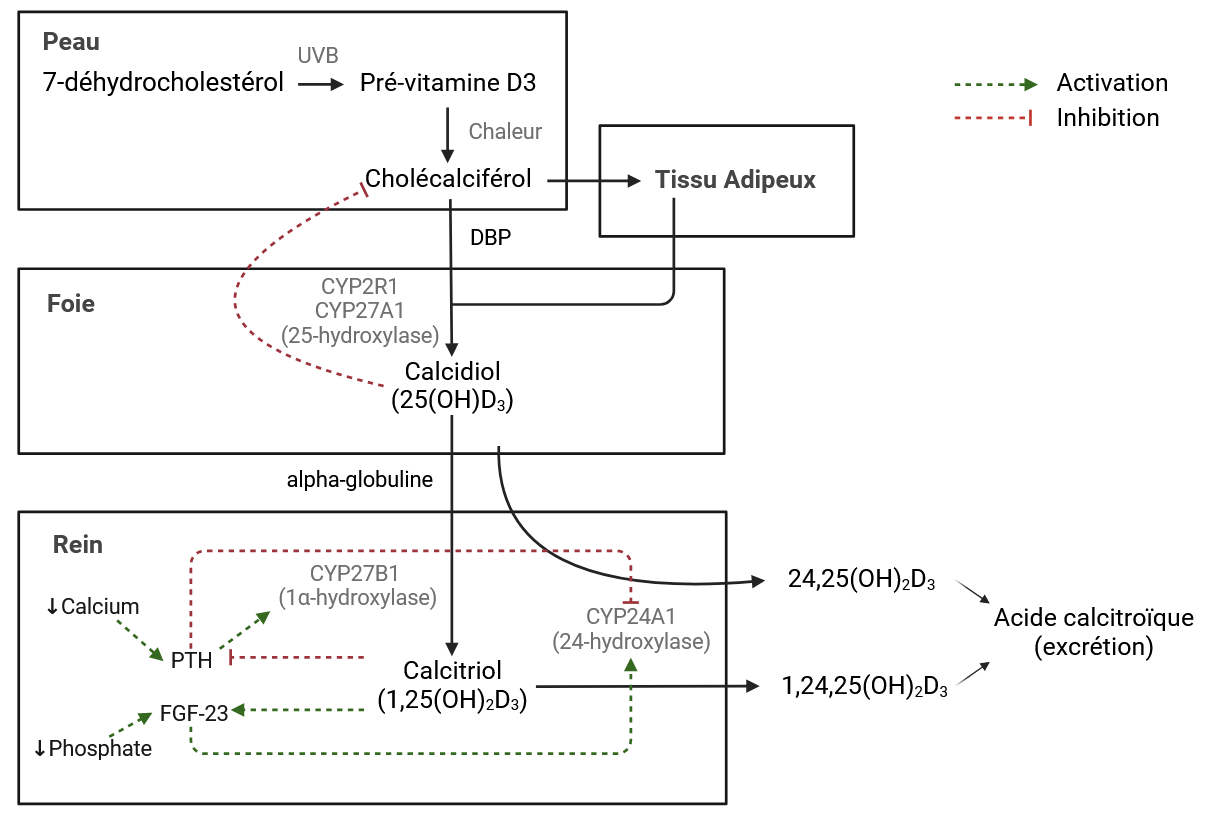
\includegraphics{figures/vitd-metabolism-fr.png}

}

\caption[Métabolisme de la vitamine
D.]{\label{fig-vitd-metabolism}\textbf{Métabolisme de la vitamine D.} Le
métabolisme de la vitamine D débute lorsque le 7-déhydrocholestérol,
présent dans la peau, est transformé par les rayons ultraviolets
provenant du soleil en cholécalciférol. Le cholécalciférol ou vitamine
D\textsubscript{3} est ensuite transporté par la protéine de liaison à
la vitamine D, et est métabolisé dans le foie par des enzymes
25-hydroxylases telles que le CYP2R1 en calcidiol ou \ac{25(OH)D3}.
L'autre étape du métabolisme se situe dans le rein, où après transport
du calcidiol, celui-ci se retrouve métabolisé en calcitriol ou
\ac{1,25(OH)2D3} par la \ac{CYP27B1}. \ac{DBP}, \acl{DBP}. La CYP24R1
est responsable du catabolisme de la vitamine D en métabolisant le
calcidiol et calcitriol en \ac{24,25(OH)2D3} et \ac{1,24,25(OH)3D3}
respectivement, où ils seront ensuite métabolisé par la même enzyme en
acide calcitroïque, qui sera excrété dans la bile du foie pour être
éliminé. D'après \textcite{Dankers.2017}, \textcite{Tsiaras.2011},
\textcite{Christakos.2010}, et \textcite{Prosser.2004}}

\end{figure}%

La synthèse du calcitriol est régulée par deux hormones, l'\acf{PTH} et
l'hormone de croissance des fibroblastes 23 (\acsu{FGF23}). La
\ac{FGF23}, induit par une concentration élevée de calcitriol et une
faible concentration de phosphate dans le sang, favorise l'induction de
la \ac{CYP24A1}, tandis que la \ac{PTH}, induite par une faible
concentration de calcium et inhibée par une forte concentration de
calcitriol, va induire la \ac{CYP27B1} et donc contribuer à la synthèse
du calcitriol \autocite{Dankers.2017,Christakos.2010}. La \ac{PTH} agit
également directement sur les os en augmentant la résorption osseuse et
augmentant ainsi la calcémie.

\section{Place de l'ergostérol}\label{place-de-lergostuxe9rol}

L'ergostérol ou vitamine D\textsubscript{2} est une autre forme de
vitamine D (\Cref{fig:ergo-struc}). Si les deux formes de vitamine sont
perçues comme interchangeables, la vitamine D\textsubscript{3} est
toutefois considérée plus intéressante en termes de traitement, car son
administration est plus efficace que celle de la vitamine
D\textsubscript{2} afin d'augmenter la concentration de calcidiol et
donc pour traiter les carences. En effet, la vitamine
D\textsubscript{2}, de nature végétale ou fongique, possède une
structure légèrement différente de la vitamine D\textsubscript{3}.

La métabolisation est fonctionnellement différente entre la vitamine
D\textsubscript{2} et vitamine D\textsubscript{3}. Ainsi, lors du
catabolisme de la vitamine D\textsubscript{2}, la 24-hydroxylation du
25(OH)D\textsubscript{2} et du
1,25(OH)\textsubscript{2}D\textsubscript{2} dans le rein conduit aux
métabolites 24,25(OH)\textsubscript{2}D\textsubscript{2} et
1,24,25(OH)\textsubscript{3}D\textsubscript{2} respectivement. Le
1,24,25(OH)\textsubscript{3}D\textsubscript{2} est inactif à la
différence de son analogue \ac{1,24,25(OH)3D3} qui nécessite une
oxydation supplémentaire afin d'être désactivée, et possède entre autres
une affinité pour le \ac{VDR} (jusqu'à 40 \% plus forte que
\ac{1,25(OH)2D3}). De plus, la 24-hydroxylation pourrait également avoir
lieu dans le foie, conduisant à la formation de
24(OH)D\textsubscript{2}. Le métabolite en résultant, la
1,24(OH)\textsubscript{2}D\textsubscript{2}, est moins affin pour le
\ac{VDR} comparé à son analogue D\textsubscript{3}. En revanche, la
vitamine D\textsubscript{3} ne subit pas cette première 24-hydroxylation
hépatique \autocite{Houghton.2006}. 1

\begin{figure}[ht]
\centering

\includegraphics[width=0.8\textwidth]{figures/ergo_vs_chole.png}
\caption[Comparaison de la structure de l'ergocalciférol par rapport au cholécalciférol.]{\textbf{Comparaison de la structure de l'ergocalciférol par rapport au cholécalciférol.} La structure de l'ergocalciférol comprend une double liaison et un groupement méthyl (CH\textsubscript{3}) supplémentaire par rapport au cholécalciférol. Cela implique une voie de métabolisation différente, notamment une voie d'élimination plus rapide, et donc une diminution de la concentration en métabolite biologiquement actif issue de l'ergocalciférol \autocite{Houghton.2006}.}
\label{fig:ergo-struc}

\vspace{1em}

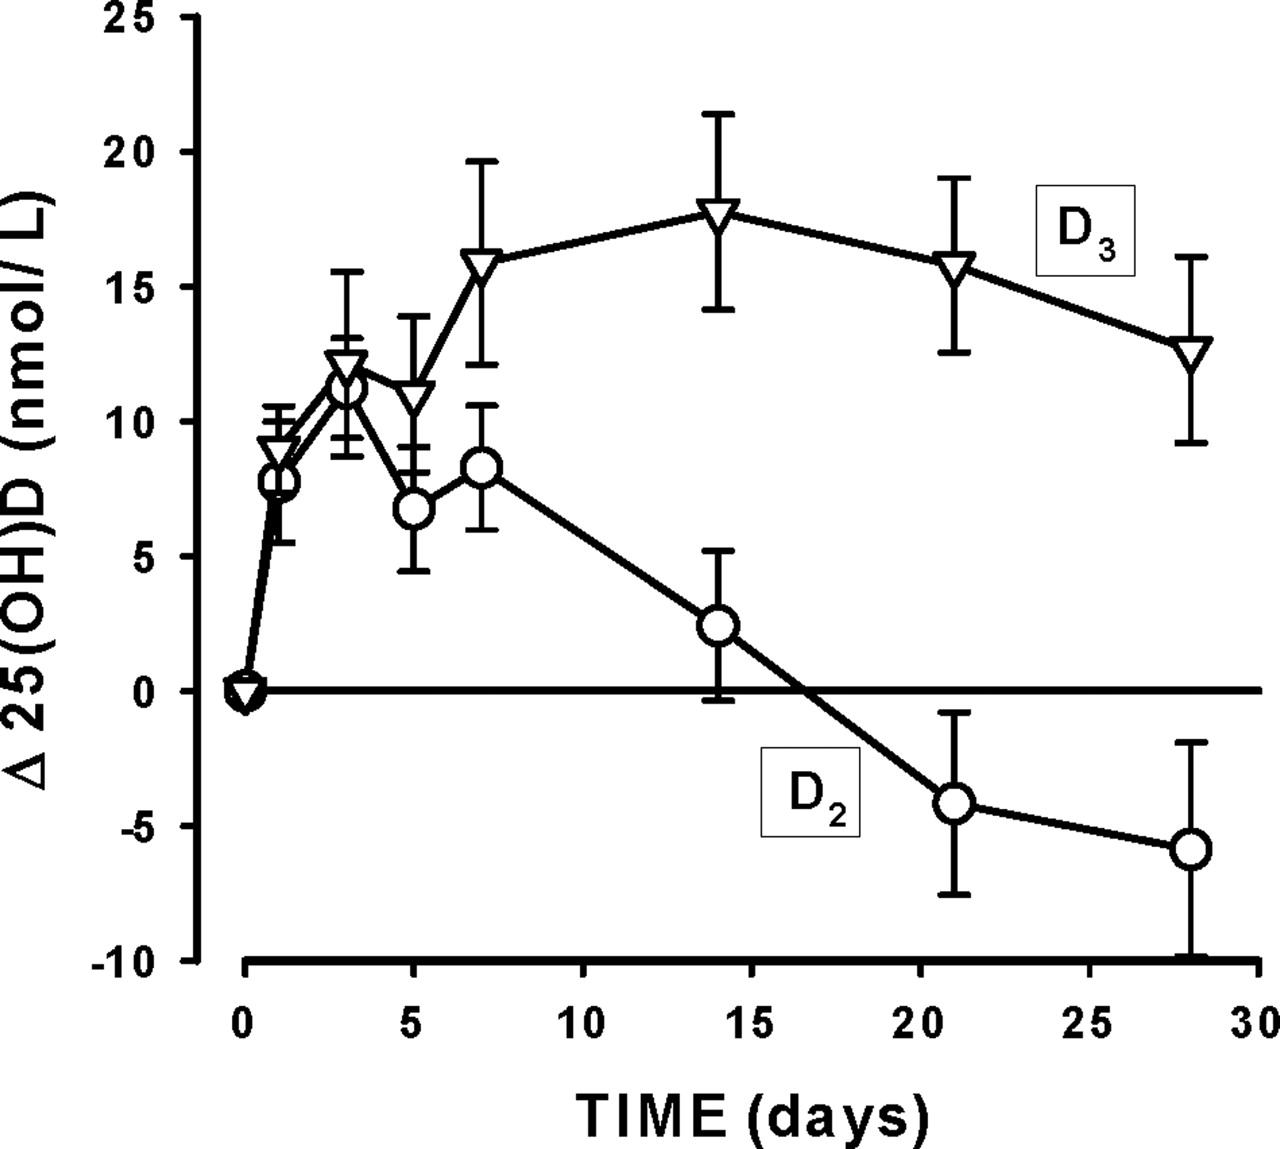
\includegraphics[width=0.8\textwidth]{figures/PK_D2_vs_D3.jpeg}
\caption[Evolution de la concentration en 25(OH)D après administration d'une dose de 50 000 UI de vitamine D\textsubscript{2} ou D\textsubscript{3} chez 10 patients.]{\textbf{Evolution de la concentration en 25(OH)D après administration d'une dose de 50 000 UI de vitamine D\textsubscript{2} ou D\textsubscript{3} chez 10 patients} \autocite{Armas.2004}.}
\label{fig:PK}
\end{figure}

De ce fait, la vitamine D\textsubscript{2} possède une pharmacocinétique
différente. La mesure de la capacité des deux formes de vitamine D à
maintenir les concentrations en \ac{25(OH)D} suite à l'administration
d'une dose de 50 000 UI des deux types de vitamine D (\Cref{fig:PK})
montre que la vitamine D\textsubscript{2} est inférieure à la vitamine
D\textsubscript{3}, malgré une phase d'absorption identique les trois
premiers jours, du fait d'une élimination beaucoup plus rapide
\autocite{Armas.2004}.

Selon les auteurs et la dose administrée, la vitamine D\textsubscript{3}
serait deux à trois fois plus efficace que la vitamine
D\textsubscript{2} pour augmenter la concentration en 25(OH)D
\autocite{Trang.1998,Armas.2004}.

L'ergocalciférol continue d'être utilisée en tant que supplément aux
Etats-Unis \autocite{Houghton.2006}. Cependant, cette forme de
traitement reste moins efficace voire est insuffisante pour corriger les
déficits en vitamine D comparée au cholécalciférol, comme le montre
certains essais cliniques \autocite{Boyle.2005}.

Le cholécalciférol étant la forme de vitamine D possédant une meilleure
capacité à augmenter la concentration de calcidiol à long terme, il
devrait être privilégié lors de supplémentations. Pour ces raisons, nous
ne discuterons seulement que de la vitamine D\textsubscript{3} lorsque
nous examinerons l'usage et le potentiel thérapeutique de la vitamine D.

\section{Propriétés}\label{propriuxe9tuxe9s}

\subsection{Propriétés classiques
osseuses}\label{propriuxe9tuxe9s-classiques-osseuses}

L'usage de la vitamine D précède sa découverte avec l'utilisation de
l'huile de foie de morue décrite dans la littérature dès 1782 par Thomas
Percival, qui rapporte son usage et les effets bénéfiques constatés sur
le rhumatisme chronique en Angleterre 1782 par \autocite{Percival.1782}.
A cette époque, se multiplient chez l'enfant les cas de rachitisme, une
maladie caractérisée par le ramollissement et l'affaiblissement des os.
En France, Armand Trousseau compile en 1858 le Traité de thérapeutique
et de matière médicale, qui reprend les opinions contemporaines sur la
matière médicale et ses expériences, et décrit l'action thérapeutique de
l'usage de l'huile de foie de morue sur le rachitisme et fait
remarquablement disparaître tous les symptômes
\autocite{Trousseau.1858}. Il publie également son ouvrage Clinique
Médicale de l'Hôtel-Dieu en 1861, où il déclare que le rachitisme est
causé par une alimentation déséquilibrée que l'huile de foie de morue
peut résoudre \autocite{Hernigou.2019}. Le livre a été traduit en
anglais et est devenu célèbre \autocite{Hernigou.2019}.

Dans les années 1917--1922, les progrès concernant les causes et le
traitement du rachitisme se sont accélérées. \textcite{Hess.1917.lc}
démontrent que l'administration de l'huile de foie de morue permet de
prévenir et guérir du rachitisme chez les enfants afro-américains à New
York. En 1918, Mellanby a montré qu'il était possible de prévenir le
rachitisme expérimental chez des chiots avec de l'huile de foie de morue
et évoquait le rôle d'un ``facteur accessoire'' dans la production du
rachitisme \autocite{ORiordan.2014}. Par la suite, \textcite{Hess.1921}
ont rapporté que l'exposition au soleil permettait de guérir du
rachitisme. Ce sera \textcite{McCollum.1922} qui donnera le nom de
Vitamine D au ``facteur accessoire'' proposé par Mellanby
\autocite{Hernigou.2019,Mavrotas.2021}

L'intérêt pour la vitamine D s'est ensuite accru avec la découverte par
les scientifiques de son rôle crucial dans le métabolisme du calcium et
du phosphore. Depuis lors, de nombreuses études ont été menées pour
évaluer le rôle de la vitamine D dans le métabolisme osseux, et il est
désormais largement admis que la vitamine D joue un rôle essentiel dans
le maintien de la santé des os et des dents
\autocite{IOM.2011,Goltzman.2018}. Une carence en vitamine D est
associée à un risque accru d'ostéomalacie (une affection qui entraîne
une diminution de la masse osseuse) et d'ostéoporose (une affection
caractérisée par une fragilité des os).

L'action de la vitamine D est médiée par la liaison du calcitriol au
récepteur \ac{VDR}. En effet, le \ac{VDR} est un récepteur nucléaire
agissant comme un facteur de transcription. Le calcitriol rentre dans la
cellule cible et se lie au \ac{VDR}, induisant un changement
conformationnel et permettant de se lier à un autre récepteur \ac{RXR},
créant l'hétérodimère \ac{VDR}-\ac{RXR}. Ce complexe reconnaît une
séquence génétique spécifique appelée \ac{VDRE}, où l'hétérodimère
\ac{VDR}-\ac{RXR} et module ainsi l'expression des facteurs de
transcription \autocite{Dankers.2017,Pike.2010,Valdivielso.2009}.

La vitamine D agit directement sur le renouvellement osseux mais joue
également un rôle dans l'homéostasie du calcium. Cette dernière dépend
de l'absorption du calcium dans l'intestin, de sa réabsorption dans le
rein et de sa fixation/libération dans l'os. Le calcium est absorbé
grâce à des transporteurs transcellulaires (actifs) et par diffusion
paracellulaire (passive), sous le contrôle du calcitriol. Celui-ci est
considéré comme le principal facteur régulateur de l'absorption
intestinal de calcium. Lorsque les flux de calcium sont déséquilibrés,
les os servent de réservoir de calcium afin de maintenir l'équilibre
calcique. La réabsorption du calcium par le rein est contrôlée dans le
tubule contourné distal par l'action du calcitriol sur le \ac{VDR}
\autocite{Carmeliet.2015}. Ainsi, la vitamine D joue un rôle crucial
dans l'absorption intestinale du calcium et du phosphore, assurant ainsi
l'homéostasie du calcium et du phosphore dans l'organisme. Cependant, un
certain nombre des manifestations de la carence en vitamine D ne sont
pas totalement superposables à celles de l'invalidation du \ac{VDR}.

De plus, la liaison du calcitriol sur le VDR situé dans les ostéoblastes
entraîne une augmentation de la minéralisation osseuse et donc de la
fixation du calcium dans les os (diminution de RANKL, facteur de
transcription activant les ostéoclastes, et augmentation de LRP5)
\autocite{Carmeliet.2015}. Lorsque la calcémie est basse, l'augmentation
de la \ac{PTH} conduit à une augmentation de RANKL ce qui favorise la
résorption des os par les ostéoclastes afin d'augmenter la calcémie
(\Cref{fig-vitd-metabolism}).

\subsection{Propriétés
extra-osseuses}\label{propriuxe9tuxe9s-extra-osseuses}

La découverte des propriétés extra-osseuses de la vitamine D a commencé
avec le clonage du récepteur \ac{VDR} en 1987. Son identification dans
la majorité des tissus et populations cellulaires a ouvert la voie à de
nombreuses études fondamentales et cliniques autour du rôle pléiotrope
de la vitamine D \autocite{Rosen.2012}. Le \ac{VDR} est exprimé de façon
ubiquitaire ; cependant, certaines cellules ou tissus, tels que les
globules rouges, les muscles striés, et certaines cellules hautement
différenciés du cerveau telles que les cellules de Purkinje du cervelet,
n'expriment que faiblement \ac{VDR} \autocite{Bouillon.2008}.

Plus récemment l'intérêt pour la vitamine D a été étendu à différentes
pathologies diversement associées à des désordres osseux, en particulier
dans le cancer, les maladies cardio-métaboliques (obésité et diabète de
type 2, métabolisme du glucose) et les maladies auto-immunes (diabète de
type 1, sclérose en plaques, troubles thyroïdiens auto-immuns)
\autocite{Dankers.2017,Caprio.2017}. En effet, plusieurs recherchent
suggèrent que la vitamine D joue un rôle dans le diabète de type 2, en
stimulant l'expression des récepteurs à l'insuline et en augmentant la
sensibilité à l'insuline. Elle jouerait aussi un rôle dans l'obésité au
niveau du tissu adipeux, où des corrélations inverses ont été observées
entre le taux de calcidiol et la leptine (hormone régulant l'appétit) et
résistine (hormone pro-inflammatoire et contribue à la résistance à
l'insuline), et une association positive avec l'adiponectine (hormone
augmentant la sensibilité à l'insuline)
\autocite{Caprio.2017,Bellia.2013}. Il existe une association inverse
entre le taux de calcidiol et de marqueurs d'inflammation systémique
chez les sujets obèses \autocite{Bellia.2013}.

Un autre domaine d'intérêt concernant les effets extra-squelettiques de
la vitamine D concerne son rôle au niveau des muscles squelettiques.
Plusieurs études suggèrent que la vitamine D stimule la synthèse des
protéines musculaires ainsi que la réabsorption du calcium dans le
réticulum sarcoplasmique, ce qui permet de maintenir une force
musculaire adéquate \autocite{Caprio.2017}.

Enfin, la vitamine exercerait des effets régulateurs sur la fonction des
cellules immunitaires comme nous le verrons plus loin.

\begin{landscape}
\begin{figure}
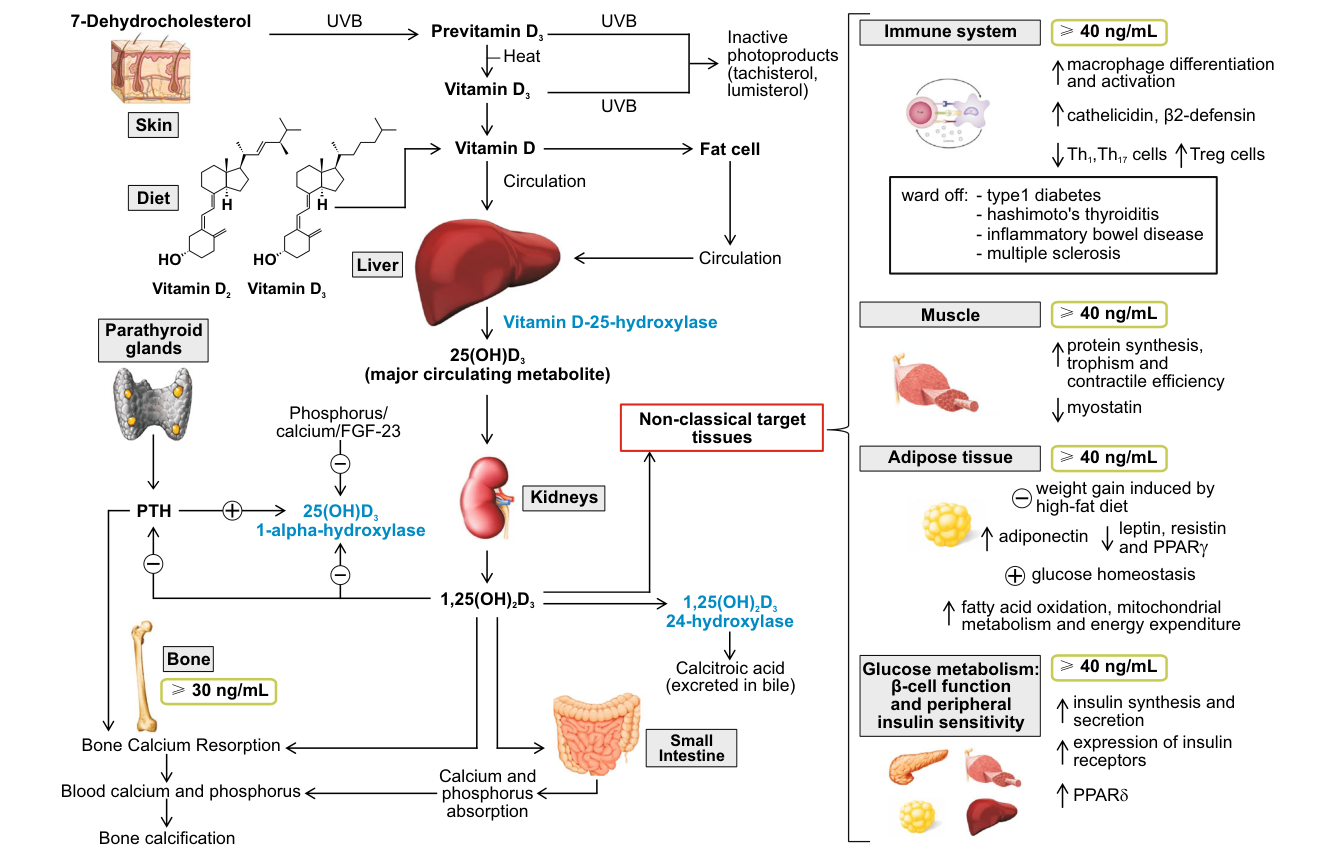
\includegraphics{figures/extra-skeletal-effect.png} 
\caption[Effets classiques et extra-squelettiques de la vitamine D.]
{\textbf{Effets classiques et extra-squelettiques de la vitamine D.} \textcite{Caprio.2017}}
\label{fig:extra-skeletal}
\end{figure}
\end{landscape}

La vitamine D exerce en plus de son action endocrine classique,
dépendante de la 1-hydroxylation par le rein, une action locale
autocrine et paracrine, par le biais d'une expression locale de
l'hydroxylase \ac{CYP27B1} dans différents tissus
\autocite{Carmeliet.2015,Cannell.2008}. Cela concerne notamment l'action
de la vitamine D sur l'immunité.

Cependant, selon certains auteurs, les bénéfices extra-squelettiques de
la vitamine D ne seraient notables que lorsque la concentration de
calcidiol serait supérieure au seuil de 20-30 ng/mL actuellement
recommandé par les autorités de santé. Les données contradictoires des
études cliniques randomisées sur les effets de la supplémentation en
vitamine D ne permettent pas de trancher
\autocite{Caprio.2017,Lewis.2015,Bouillon.2013,Rejnmark.2017}.

\section{Dose thérapeutique
efficace}\label{dose-thuxe9rapeutique-efficace}

\subsection{Unités}\label{unituxe9s}

L'expression de la dose de la vitamine D peut se faire en plusieurs
unités. Classiquement, c'est l'\ac{UI} qui est utilisée. Elle peut
également être exprimée en masse lors de prises de comprimés.
L'équivalence est de 1 µg pour 40 \ac{UI} ou 1 \ac{UI} pour 0,025 g. La
concentration de vitamine D (en fait celle de calcidiol utilisée comme
marqueur du statut vitaminique) est définie en ng/mL ou en nmol/L. Pour
passer de ng/mL en nmol/L, il suffit de multiplier par 2.5
\autocite{Pramyothin.2012}

Cependant la \ac{FDA} a décidé depuis janvier 2021 de passer à une dose
écrite en microgramme, ce qui oblige les fabricants à donner
l'information en microgramme, bien que la dénomination en UI reste
possible en parallèle \autocite{HHS.2016}.

Un essai-clinique visant à établir l'efficacité de la supplémentation en
cholécalciférol a été réalisée chez 61 patients, selon trois schémas
d'administration : 1000 UI par jour, 7000 UI par semaine ou 30 000 UI
par mois. Les patients inclus étaient carencés en début d'étude avec une
concentration de calcidiol inférieure à 20 ng/mL (en moyenne autour de
13,3 ng/mL) et ont été suivi pendant 3 mois. L'étude a permis de
déterminer que, en moyenne, une supplémentation en cholécalciférol
augmente la concentration de calcidiol de 1.3 ng/100 UI par jour
\autocite{Takács.2017}.

\subsection{Dose recommandée
journalière}\label{dose-recommanduxe9e-journaliuxe8re}

Actuellement, l'Académie américaine de médecine (anciennement Institute
of Medicine, \acsu{IOM}) est responsable des recommandations émises par
la \ac{FDA}, l'équivalent de l'\ac{ANSM} en France. L'\ac{AJR} pour la
vitamine D est de 600 UI par jour tous sexes confondus de 1 à 70 ans, et
reste le même en cas de grossesse ou d'allaitement \autocite{IOM.2011}.
L'\ac{AJR} est augmentée à 800 UI/jour chez les personnes de plus de 70
ans en raison de la plus grande variabilité des données disponibles
concernant cette catégorie d'âge. Une concentration sanguine de
calcidiol de 20 ng/mL ou plus est considérée par l'\ac{IOM} comme étant
le minimum adéquat chez 97,5 \% des personnes en bonne santé. Cette
concentration minimum de 20 ng/mL a été observé comme étant associée
pour la majorité de la population générale à une bonne santé osseuse
définie en termes de densité minérale osseuse et d'absorption du
calcium, d'accrétion et de maintenance osseuse, et de diminution du
risque d'ostéomalacie ou de rachitisme. Les concentrations de calcidiol
supérieures à 30 ng/mL ne sont pas associées à un bénéfice
supplémentaire selon l'\ac{IOM} \autocite{IOM.2011,Rosen.IOM.2012}.

Un autre acteur français, l'\ac{ANSES}, stipule que les recommandations
journalières de cholécalciférol sont de 15 µg par jour pour un adulte,
soit l'équivalent d'une dose de 600 UI/j, s'appuyant sur les
recommandations de l'Autorité européenne de sécurité des aliments
(\acsu{EFSA}) \autocite{ANSES.2021}. En effet, l'\ac{EFSA} a retenu une
valeur de 15 µg/j (soit 600 UI/j) permettant aux hommes et femmes
d'atteindre le seuil de calcidiol jugé adéquat de 50 nmol/L ou 20 ng/mL
\autocite{ANSES.2022.note} (\Cref{tbl-seuil}).

\begin{table}
\caption[Tableau comparatif des seuils d'adéquation de la vitamine D par différentes sources.]{\textbf{Tableau comparatif des seuils d'adéquation de la vitamine D par différentes sources.} IOM : Institut de Médecine ; ANSES : Agence nationale de sécurité sanitaire de l’alimentation, de l’environnement et du travail. D'après \textcite{IOM.2011} et \textcite{ANSES.2021}}
\label{tbl-seuil}
\centering
\begin{tabular}{ccc}
\toprule
\textbf{Seuil de vitamine D} & \textbf{IOM} & \textbf{ANSES}\\
\midrule
Déficience en vitamine D & < 12 ng/mL & < 10 ng/mL\\
Insuffisance en vitamine D & 12-20 ng/mL & 10-20 ng/mL\\
Valeurs recommandées & 20-30 ng/mL & 20-30 ng/mL\\
Limite Supérieure de Sécurité & > 50 ng/mL  & > 100 ng/mL \\
\bottomrule
\end{tabular}
\end{table}

\begin{table}
\centering
\caption[Apports journaliers recommandés de la vitamine D (UI/j)]{\textbf{Apports journaliers recommandés de la vitamine D (UI/j).} La mention d'\ac{AJR} indique que l'apport couvre les besoins minimum de 97,5 \% de la population pour atteindre une concentration de 20 ng/mL selon l'\ac{IOM}. D'après \textcite{ANSES.2021, IOM.2011}}
\label{tbl-AJR}
\begin{tabular}{ccc}
\toprule
\textbf{Groupe d'âge} & \textbf{IOM} & \textbf{ANSES/EFSA} \\
\midrule
Nourrissons (0-12 mois) & 400 & 400 \\
Enfants (1 - 11 ans) & 600 & 600 \\
Adolescents (11 - 17 ans) & 600 & 600 \\
Hommes et Femmes & 800 & 600 \\
Femmes enceintes & 600 & 600 \\
\bottomrule
\end{tabular}
\end{table}

\subsection{Controverse autour de la dose recommandée
journalière}\label{controverse-autour-de-la-dose-recommanduxe9e-journaliuxe8re}

Plusieurs acteurs tels que la Société d'Endocrinologie suggèrent que les
\ac{AJR} établis par l'\ac{IOM} sont insuffisants. La Société
d'Endocrinologie suggère un \ac{AJR} de 1500 UI/j pouvant aller à 2000
UI/j pour des adultes, avec des recommandations ciblées pour des
populations à risque avec des maladies spécifiques pour lesquelles le
seuil minimal de calcidiol serait de 30 ng/mL. L'\ac{IOM} suggère dans
une réponse à la Société d'Endocrinologie que les auteurs ont fait un
amalgame entre apports nutritionnels pour la population générale et
l'établissement des recommandations pour des personnes à risque, ce qui
inclut des conditions adéquates pour la population générale
\autocite{Rosen.IOM.2012}. De plus, l'\ac{IOM} est en désaccord en qui
concerne les bénéfices osseux, concluant sur la base de la littérature
qu'il n'y a pas de bénéfices osseux observés au-delà de 20 ng/mL, qui
est le seuil permettant de couvrir les besoins minimes de 97,5 \% de la
population (\Cref{tbl-seuil}). L'\ac{IOM} conclut que les bénéfices
extra-squelettiques de la vitamine D sont incertains et que les preuves
ne sont pas suffisantes pour recommander une augmentation de l'\ac{AJR}
\autocite{IOM.2011}.

\section{Utilisation thérapeutique}\label{utilisation-thuxe9rapeutique}

La vitamine D est surtout utilisée en thérapeutique afin de prévenir les
carences à des fins de bonne santé osseuse. Elle permet de prévenir le
rachitisme chez les enfants et l'ostéoporose chez les adultes et surtout
chez les personnes âgées. Elle permet de maintenir une bonne densité
osseuse et une absorption du calcium adéquat et prévient du rachitisme
et de l'ostéomalacie.

La vitamine D possède également un potentiel thérapeutique dans le
traitement des maladies auto-immunes. De ce fait, le groupe clinique
dirigé par Cicero Coimbra au Brésil utilise de fortes doses quotidiennes
de vitamine D, allant de 40 000 UI à 300 000 UI, pour traiter la
sclérose en plaques et le vitiligo. Le statut clinique des patients
atteints de psoriasis et le degré de repigmentation chez les patients
atteints de vitiligo s'améliorent de manière significative
\autocite{Amon.2022}. Néanmoins, il s'agit d'une circonstance
particulière où cette approche repose sur l'hypothèse que ces maladies
auto-immunes sont dues à une résistance à la vitamine D
\autocite{Lemke.2021}.

De plus, les analogues de la vitamine D sont utilisés dans le traitement
de la psoriasis tel que le talcacitol, en première ligne seul ou en
combinaison avec des corticostéroïdes topiques. Contrairement aux
corticostéroïdes, le talcacitol n'induit pas d'accoutumance et ne
provoque pas d'effets indésirables \autocite{Giustina.2020}.

\section{Pharmacocinétique}\label{pharmacocinuxe9tique}

La pharmacocinétique de la vitamine D est beaucoup plus complexe que
celle d'un agent pharmacologique standard, en raison de l'hydroxylation
progressive nécessaire pour obtenir sa forme active, et de la présence
de ses métabolites dans la circulation et les tissus. De plus, sa
liaison à son transporteur \acsu{DBP} influence les propriétés des
métabolites de la vitamine D \autocite{Schoenmakers.2018}. Comme nous
l'avons vu (\textbf{Section~\ref{sec-metabolisme}}), la vitamine D est
hydroxylée en calcidiol par le CYP2R1, une enzyme possédant une haute
capacité de métabolisation : la demi-vie de la vitamine D non hydroxylée
est donc faible et il est possible d'observer le cholécalciférol en
concentration substantielle dans le plasma lors que la dose sature la
capacité de l'enzyme \autocite{Schoenmakers.2018}.

\begin{figure}

\centering{

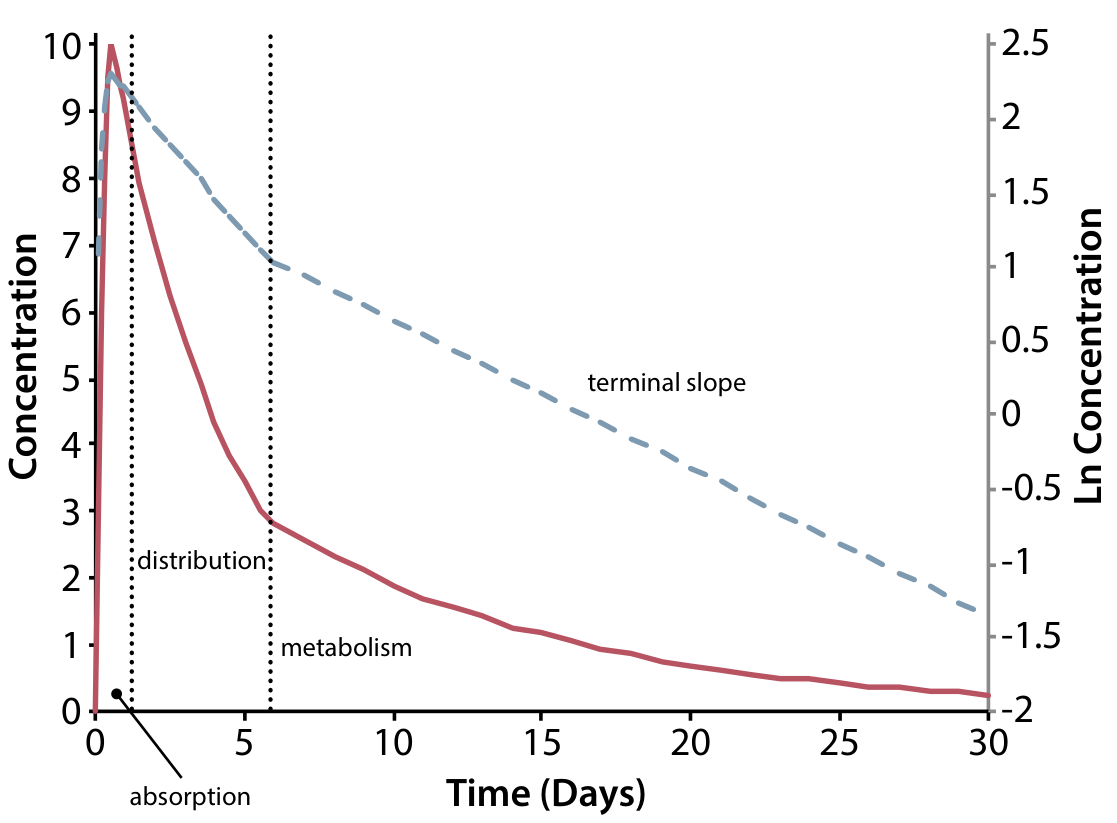
\includegraphics{figures/Schoenmakers.2018 - Plasma appearance and disappearance of 25(OH)D after oral intake.png}

}

\caption[Schéma des phases pharmacocinétiques du
cholécalciférol]{\label{fig-PK-all-VitD}\textbf{Schéma des phases
pharmacocinétiques du} \ac{25(OH)D3}. La ligne pointillée correspond au
logarithme naturel de la concentration duquel les différentes pentes et
les demi-vies sont calculées. \autocite{Schoenmakers.2018}}

\end{figure}%

\subsection{Absorption}\label{absorption}

La vitamine D (en tant que cholécalciférol) possède une absorption
rapide et linéaire, atteignant la \ac{Cmax} pour une dose de vitamine
D\textsubscript{3} à un \ac{Tmax} de 6 à 10 heures. Le calcidiol est
absorbé plus rapidement que le cholécalciférol, avec un \ac{Tmax} de 4 à
6 heures (\Cref{fig-PK-all-VitD}) \autocite{Schoenmakers.2018}.

Le cholécalciférol absorbé dans le tractus digestif, suit la même voie
d'absorption que les autres substances liposolubles. Le cholécalciférol
passe par les entérocytes où il se retrouve associée aux chylomicrons.
Elle peut puis est redistribuée entre les lipoprotéines, et enfin est
transférée vers la protéine de transport principale, la \ac{DBP}
(\Cref{fig-vd-absorption}). Le cholécalciférol associé au chylomicron
peut être transféré à la \ac{DBP} ou passer dans la circulation
sanguine.

Le calcidiol quant à lui est absorbé en majeure partie par la veine
porte du foie en diffusant à travers l'entérocyte et en mineure partie
absorbée par les chylomicrons. La majorité des métabolites de la
vitamine D, dont le calcidiol, est lié à la \ac{DBP}( à environ (85 \%),
et plus faiblement à l'albumine (15 \%) \autocite{Bikle.2017}.

\begin{figure}

\centering{

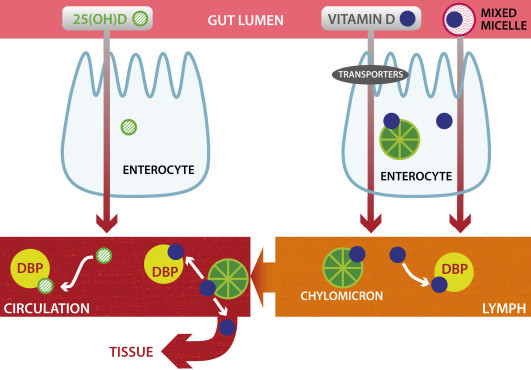
\includegraphics{figures/Schoenmakers.2018-vd-absorption.jpg}

}

\caption[Schéma de l'absorption de la vitamine D et du
calcidiol.]{\label{fig-vd-absorption}\textbf{Schéma de l'absorption de
la vitamine D et du calcidiol} \autocite{Schoenmakers.2018}. Le
cholécalciférol passe par des transporteurs actifs dans les entérocytes
où il se retrouve associé aux chylomicrons. Après être relâché dans la
lymphe, le cholécalciférol peut être transféré au \ac{DBP} ou suivre le
métabolisme du chylomicron qui peut relâcher le cholécalciférol dans les
tissus. Le calcidiol diffuse à travers l'entérocyte où il est lié en
grande majorité au \ac{DBP} plasmatique. \ac{DBP}, \acl{DBP}}

\end{figure}%

\subsection{Distribution}\label{distribution}

La vitamine D étant une molécule liposoluble, elle est principalement
distribuée dans les tissus adipeux où elle sert de compartiment de
stockage, mais également les tissus musculaires. Elle peut se retrouver
dans divers autres tissus tels que la peau, le plasma et d'autres
organes. Dans les réserves adipeuses vitamine D peut varier
considérablement entre 10 à 900 nmol/kg et il a été mesuré dans une
étude que le calcidiol pouvait varier de 2,3 à 12,8 nmol/kg. Une
corrélation positive existe entre la concentration de cholécalciférol
plasmatique et adipeuse mais elle n'est pas constamment retrouvée pour
le calcidiol.

Il n'existe pas encore d'études concernant la concentration de la
vitamine D dans les muscles chez les humains, mais des études conduites
sur des porcs nous permettent de faire des observations et
approximations. Ainsi, les muscles détiennent autour de 10\%--20\% du
cholécalciférol distribuée dans les tissus adipeux. Le ratio du
calcidiol entre le tissu adipeux et le muscle est plus élevé, variant
entre 0.5 à 1 en fonction de l'alimentation et du type de fibre
musculaire (rouge ou blanche). La concentration de calcidiol varie entre
75\% et 150\% du cholécalciférol présent dans les tissus adipeux
\autocite{Schoenmakers.2018}. La vitamine D étant une molécule
liposoluble et se distribuant abondamment dans les tissus adipeux, il
est possible de considérer que ce compartiment de distribution ait un
impact sur la pharmacocinétique de la vitamine D; le tissu adipeux
fonctionnerait comme un lieu de stockage et libèrerait de la vitamine D
sur le long terme dans la circulation sanguine.

Des données récentes suggèrent que la perte de poids n'influence pas le
statut en vitamine D. De plus, il n'est pas certain que la mobilisation
de la vitamine D et du calcidiol repose sur la diffusion de la forme
libre ou liée, ou qu'elle soit régulée, et l'impact de la masse adipeuse
sur la pharmacocinétique de la vitamine D est encore méconnu
\autocite{Schoenmakers.2018}.

Cependant il est connu que la dose nécessaire de vitamine D à
administrer pour atteindre le seuil thérapeutique doit augmenter lorsque
la masse graisse augmente, puisqu'un des compartiments de distribution
est plus grand, représenté par la masse graisseuse. La relation entre
l'\ac{IMC} a été étudiée par \textcite{Ekwaru.2014}. Ekwaru montre ainsi
la relation dose-réponse entre l'administration orale de cholécalciférol
et la concentration plasmatique de calcidiol pour l'ensemble des
individus (\Cref{subfig:vd-dose-response}), puis lorsque les sujets sont
classés selon leur \ac{IMC} (\Cref{subfig:vd-dose-imc}). Les auteurs
observent une relation dose-réponse exponentielle, où l'augmentation de
la concentration sérique de calcidiol diminue avec l'augmentation des
niveaux de supplémentation orale en vitamine D. Ils observent également
que les sujets ayant un \ac{IMC} plus élevé ont besoin d'une dose plus
élevée de vitamine D pour atteindre le même niveau de concentration
plasmatique de calcidiol.

\begin{figure}[H]
    \centering
    \begin{subfigure}{0.48\textwidth}
        \centering
        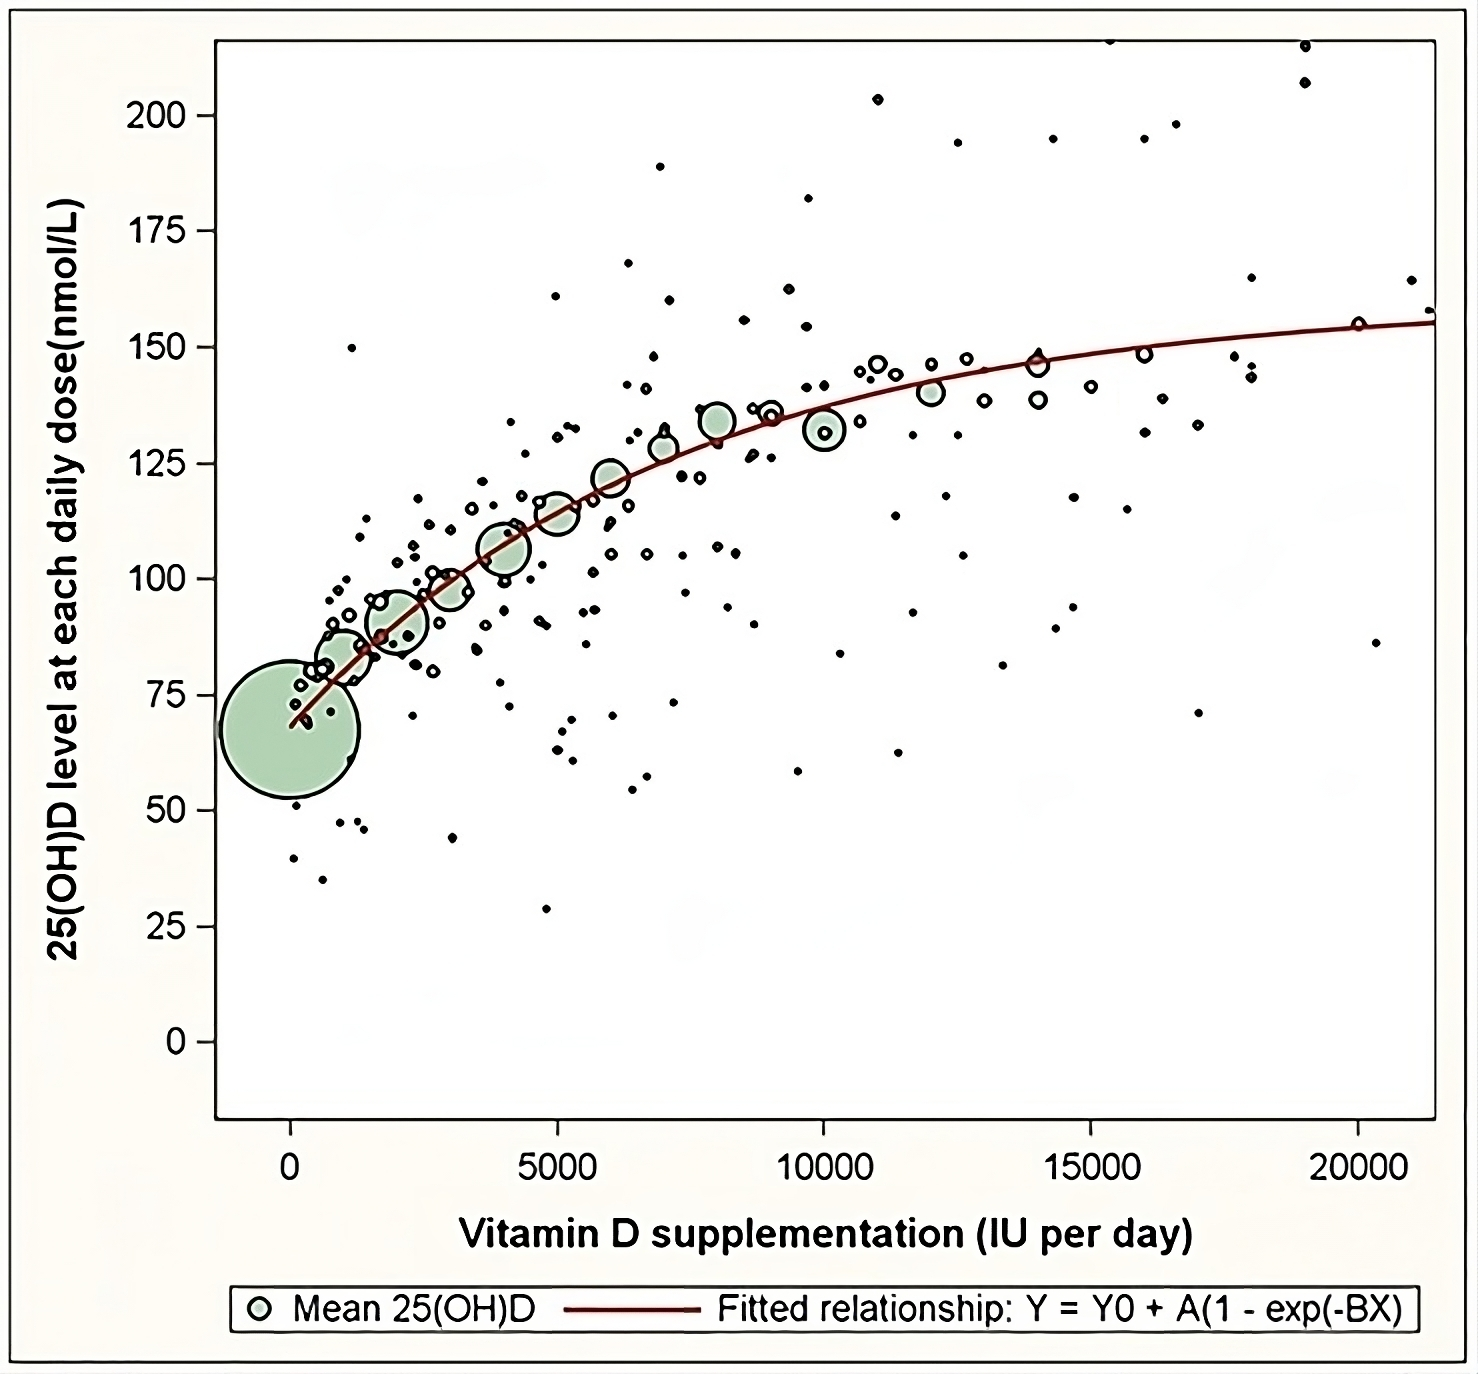
\includegraphics[width=\textwidth]{figures/ekwaru-dose-relation-transformed.jpg}
        \subcaption{Courbe dose-réponse de la supplémentation orale en vitamine D \ac{25(OH)D3} \autocite{Ekwaru.2014}.}
        \label{subfig:vd-dose-response}
    \end{subfigure}
    \hfill
    \begin{subfigure}{0.48\textwidth}
        \centering
        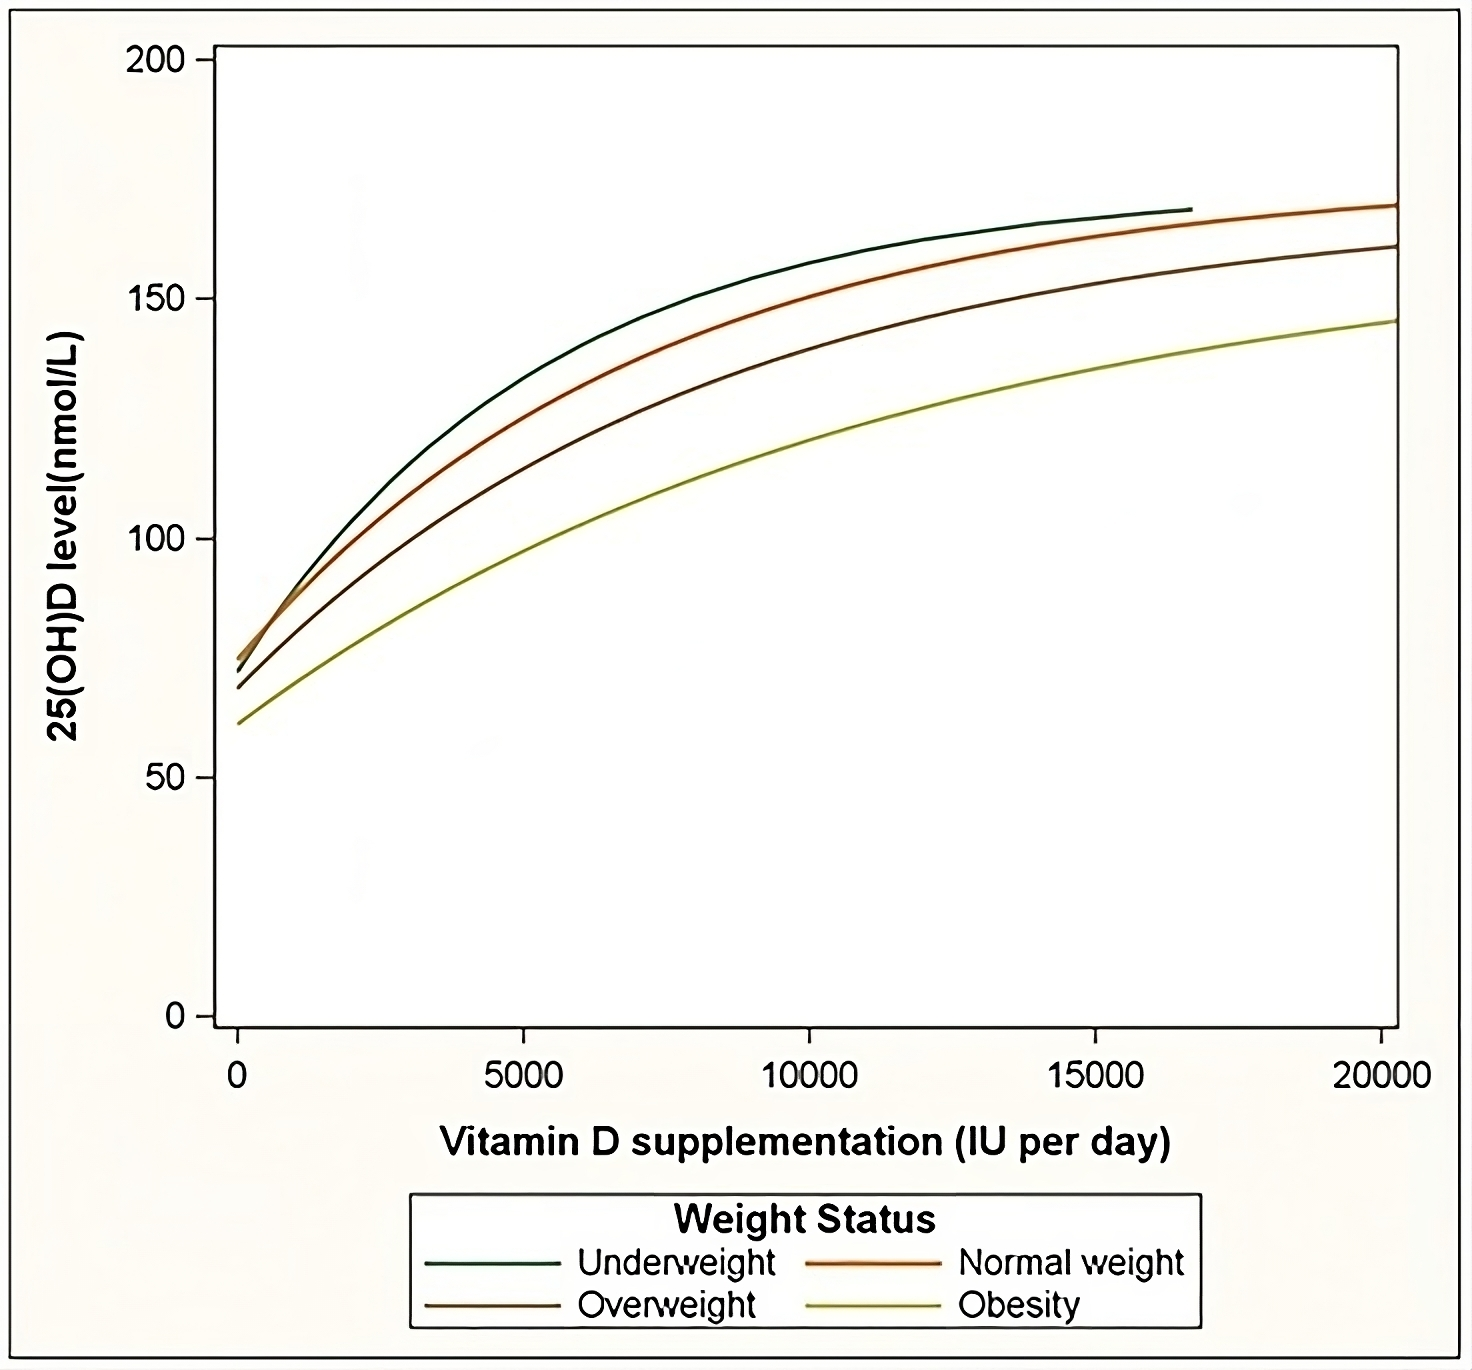
\includegraphics[width=\textwidth]{figures/ekwaru-dose-imc-transformed.jpg}
        \subcaption{Comparaison des courbes dose-réponse en fonction de l’indice de masse corporelle \autocite{Ekwaru.2014}.}
        \label{subfig:vd-dose-imc}
    \end{subfigure}
    \caption[Courbes dose-réponse de la supplémentation en vitamine D orale.]{\textbf{Courbes dose-réponse de la supplémentation en vitamine D orale.}}
    \label{fig:dose-response}
\end{figure}

Les auteurs notent que l'\ac{IMC} est un meilleur indicateur que le
poids absolu afin de juger de la quantité de vitamine D à administrer.
L'\ac{IOM} confirme également cette relation non linéaire avec une
augmentation plus marquée des concentrations sériques de calcidiol à des
doses inférieures à 1000 UI/j. La réponse est plus aplatie lorsque les
doses sont supérieures à 1000 UI/j \autocite{IOM.2011,Garland.2011}. De
ce fait, l'augmentation en vitamine D obtenue par supplémentation est
moindre lorsque la concentration initiale de vitamine D est plus élevée
(\Cref{fig:vd-expected-rise}).

\begin{figure}[H]
\centering
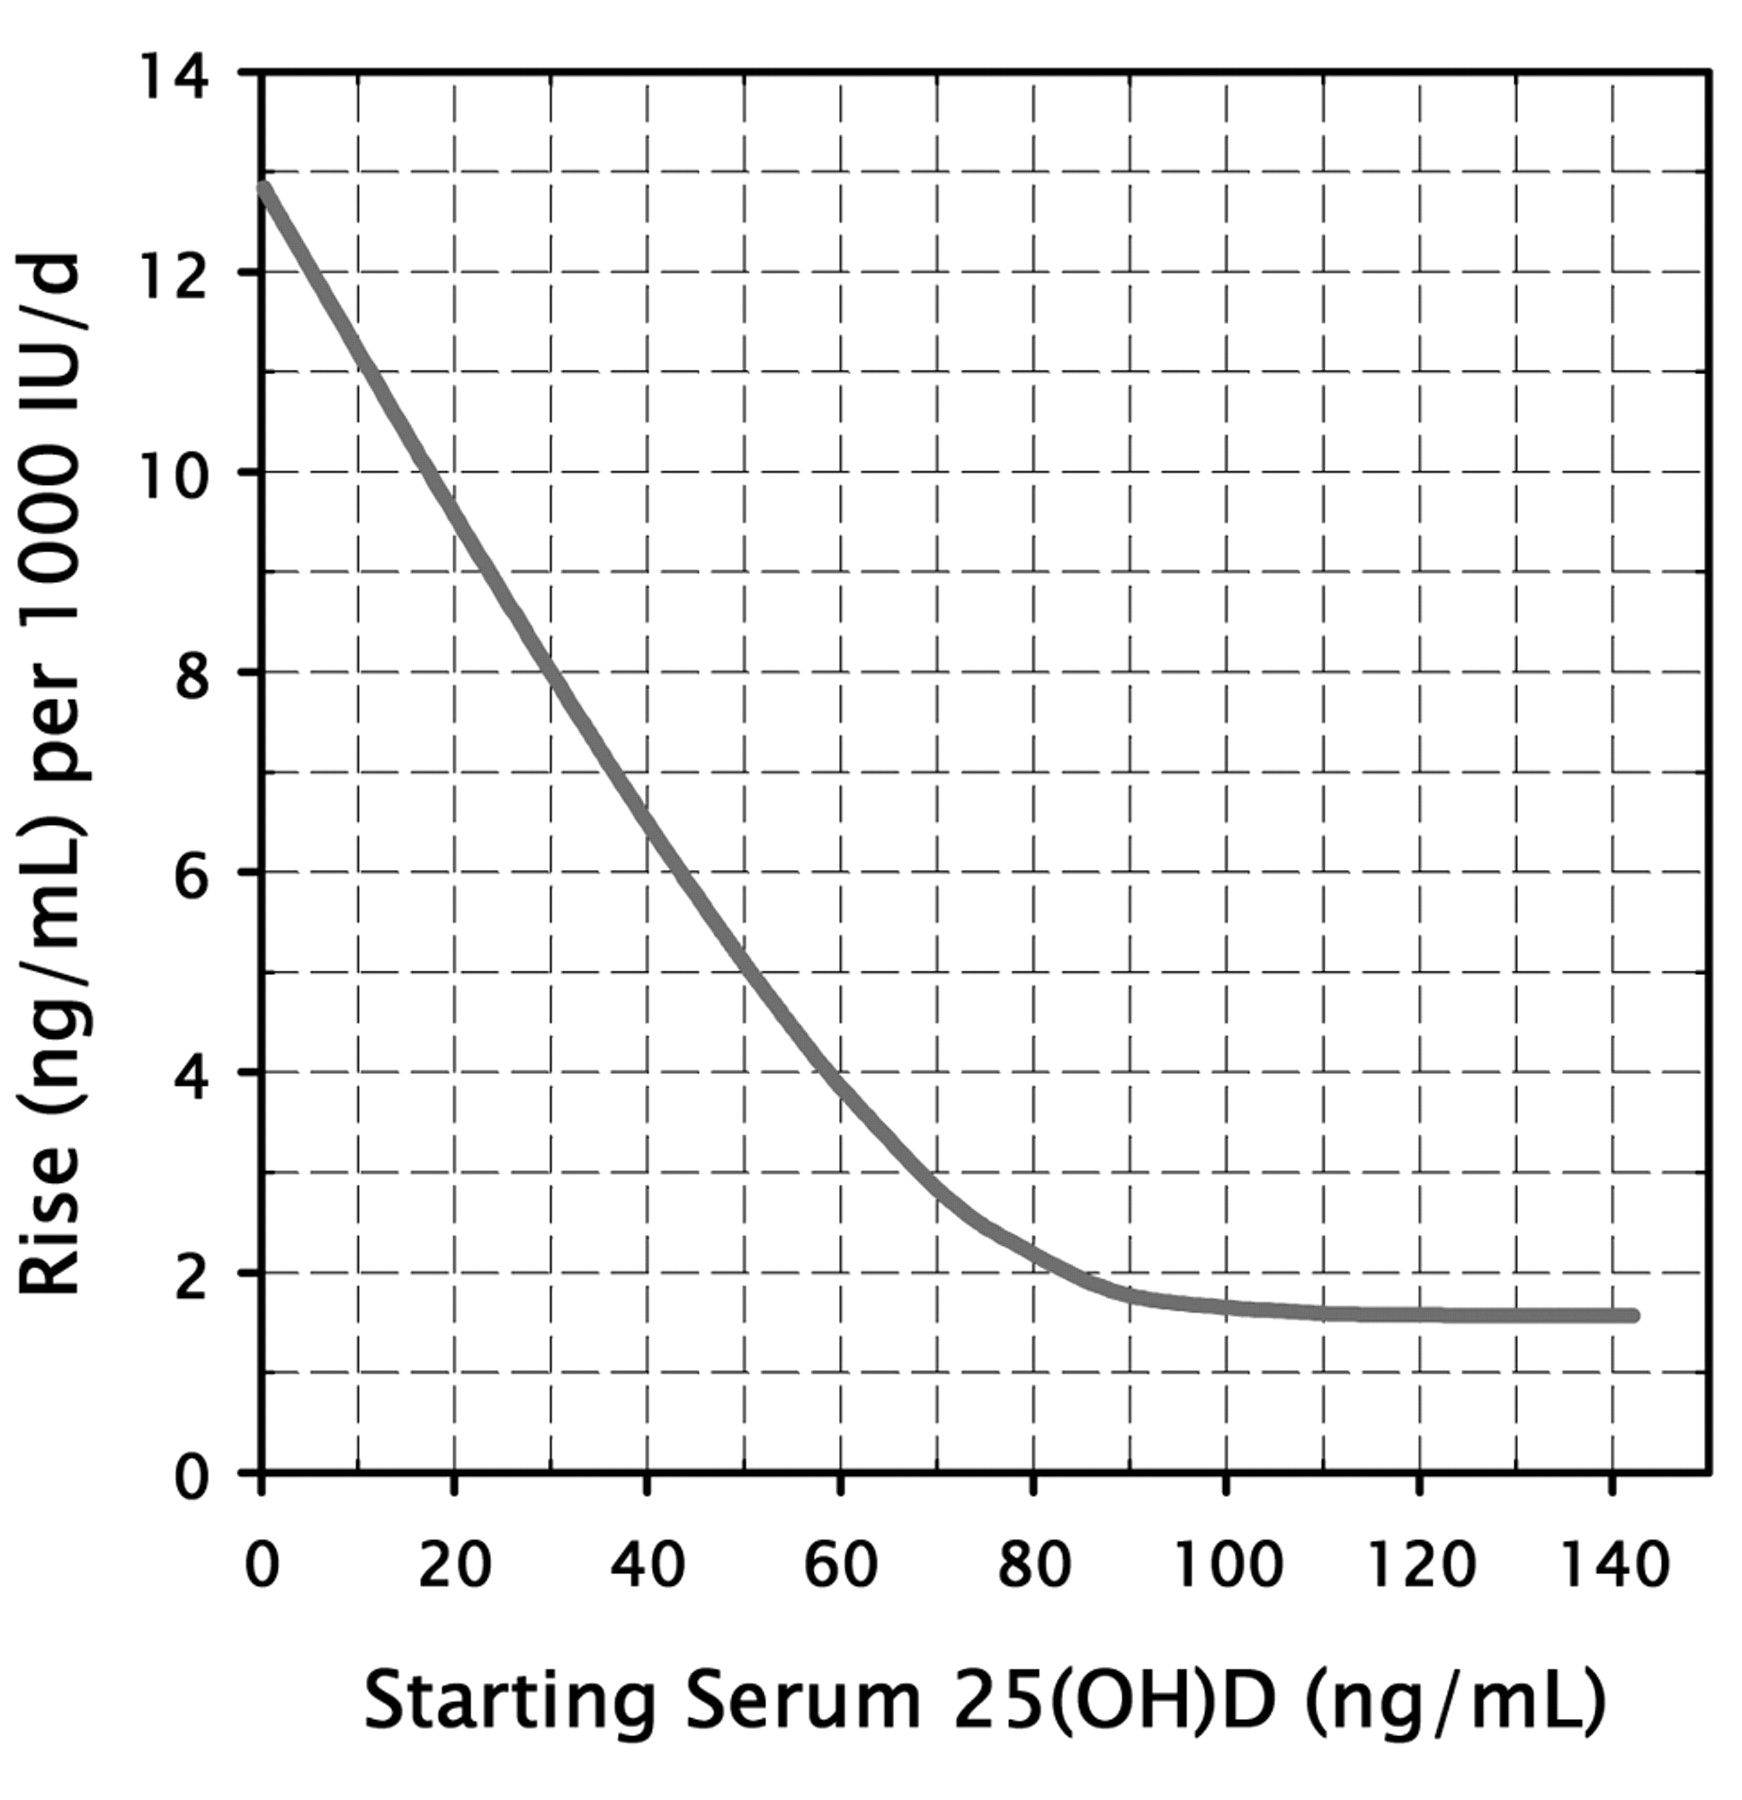
\includegraphics[width=0.5\textwidth]{figures/vd-expected-rise.jpeg}
\caption[Courbe de l'augmentation attendue de la 25(OH)D sérique pour chaque supplément de 1,000 UI de vitamine D3 par jour, en fonction de la valeur de base de la 25(OH)D de base]{\textbf{Courbe de l'augmentation attendue de la 25(OH)D sérique pour chaque supplément de 1,000 UI de vitamine D3 par jour, en fonction de la valeur de base de la 25(OH)D de base.} \autocite{Garland.2011}.}
\label{fig:vd-expected-rise}
\end{figure}

\subsection{Catabolisme et demi-vie}\label{catabolisme-et-demi-vie}

Le catabolisme de la vitamine D passe principalement par le \ac{CYP24A1}
et est exprimé universellement dans les cellules contenant le \ac{VDR}
régulant ainsi la stimulation du calcitriol sur l'expression des gènes
par son catabolisme. Elle est induite lorsque la concentration de
vitamine D devient élevée (\textgreater{} 220 nM ou 88 ng/mL). Elle
convertit ainsi le calcidiol et le calcitriol en métabolites
intermédiaires qui seront ensuite converti en acide calcitroïque par la
\ac{CYP24A1} où il sera éliminé par excrétion biliaire
\autocite{Schoenmakers.2018,Prosser.2004}.

La demi-vie du cholécalciférol est de 24 heures, et celle du calcidiol
de 10 à 40 jours, tandis que, comparativement, le calcitriol possède une
demi-vie très courte de 5 à 80 heures. Le métabolite \ac{24,25(OH)2D3}
possède quant à lui une demi-vie de 7-16 jours
\autocite{Schoenmakers.2018}. On observe ainsi que la vitamine D est
absorbée très rapidement, et se distribue rapidement dans les tissus,
mais que sa demi-vie est très longue, maintenant une concentration
plasmatique stable pendant plusieurs semaines (\Cref{fig-PK-all-VitD}).

\section{Toxicité}\label{toxicituxe9}

A dose toxique, la vitamine D induit un état hypercalcémique et
hypercalciurique, ce qui suggère un excès d'activité lié aux effets du
calcitriol \autocite{Vieth.1990}. Cet état s'accompagne d'une
suppression de l'activité de la \ac{PTH}, en raison de l'état
hypercalcémique qui exerce un rétrocontrôle négatif sur la \ac{PTH}
\autocite{Marcinowska-Suchowierska.2018,Dusso.2005}. L'apport excessif
de cholécalciférol serait corrélée à une augmentation de calcidiol qui
induirait une augmentation de l'absorption intestinale du calcium et de
la résorption osseuse \autocite{Jones.2008,IOM.2011}. Selon
\textcite{Shepard.1980}, l'hypercalcémie proviendrait probablement plus
de cette résorption osseuse plutôt que de l'absorption intestinale
accrue du calcium

La symptomatologie de cette toxicité résulte principalement de
l'hypercalcémie et de l'hyperphosphatémie
\autocite{DeLuca.2011,Janoušek.2022,Jones.2008,IOM.2011} affectant
divers organes. Les manifestations cliniques concernent notamment des
troubles gastro-intestinaux, des troubles du système cardiovasculaire
ainsi que des troubles du système musculo-squelettique. Le système rénal
est également impacté, et un trouble neurologique est également possible
(\Cref{fig-hypervitaminose-d}) \autocite{Alshahrani.2013,Janoušek.2022}.
L'hypercalcémie peut également conduire à une calcification des tissus
mous, et des vaisseaux sanguins. L'ensemble de ces conséquences
cardiovasculaires et rénales causant une défaillance de ces systèmes est
probablement à l'origine de la mortalité par intoxication à la vitamine
D. L'ensemble de ces conséquences cardiovasculaires et rénales causant
une défaillance de ces systèmes est probablement à l'origine de la
mortalité par intoxication à la vitamine D. Il est intéressant de noter
que l'hypothèse selon laquelle un apport excessif en vitamine D pourrait
être associé à la formation de calculs rénaux n'est pas appuyée par les
données disponibles \autocite{IOM.2011}

\begin{figure}

\centering{

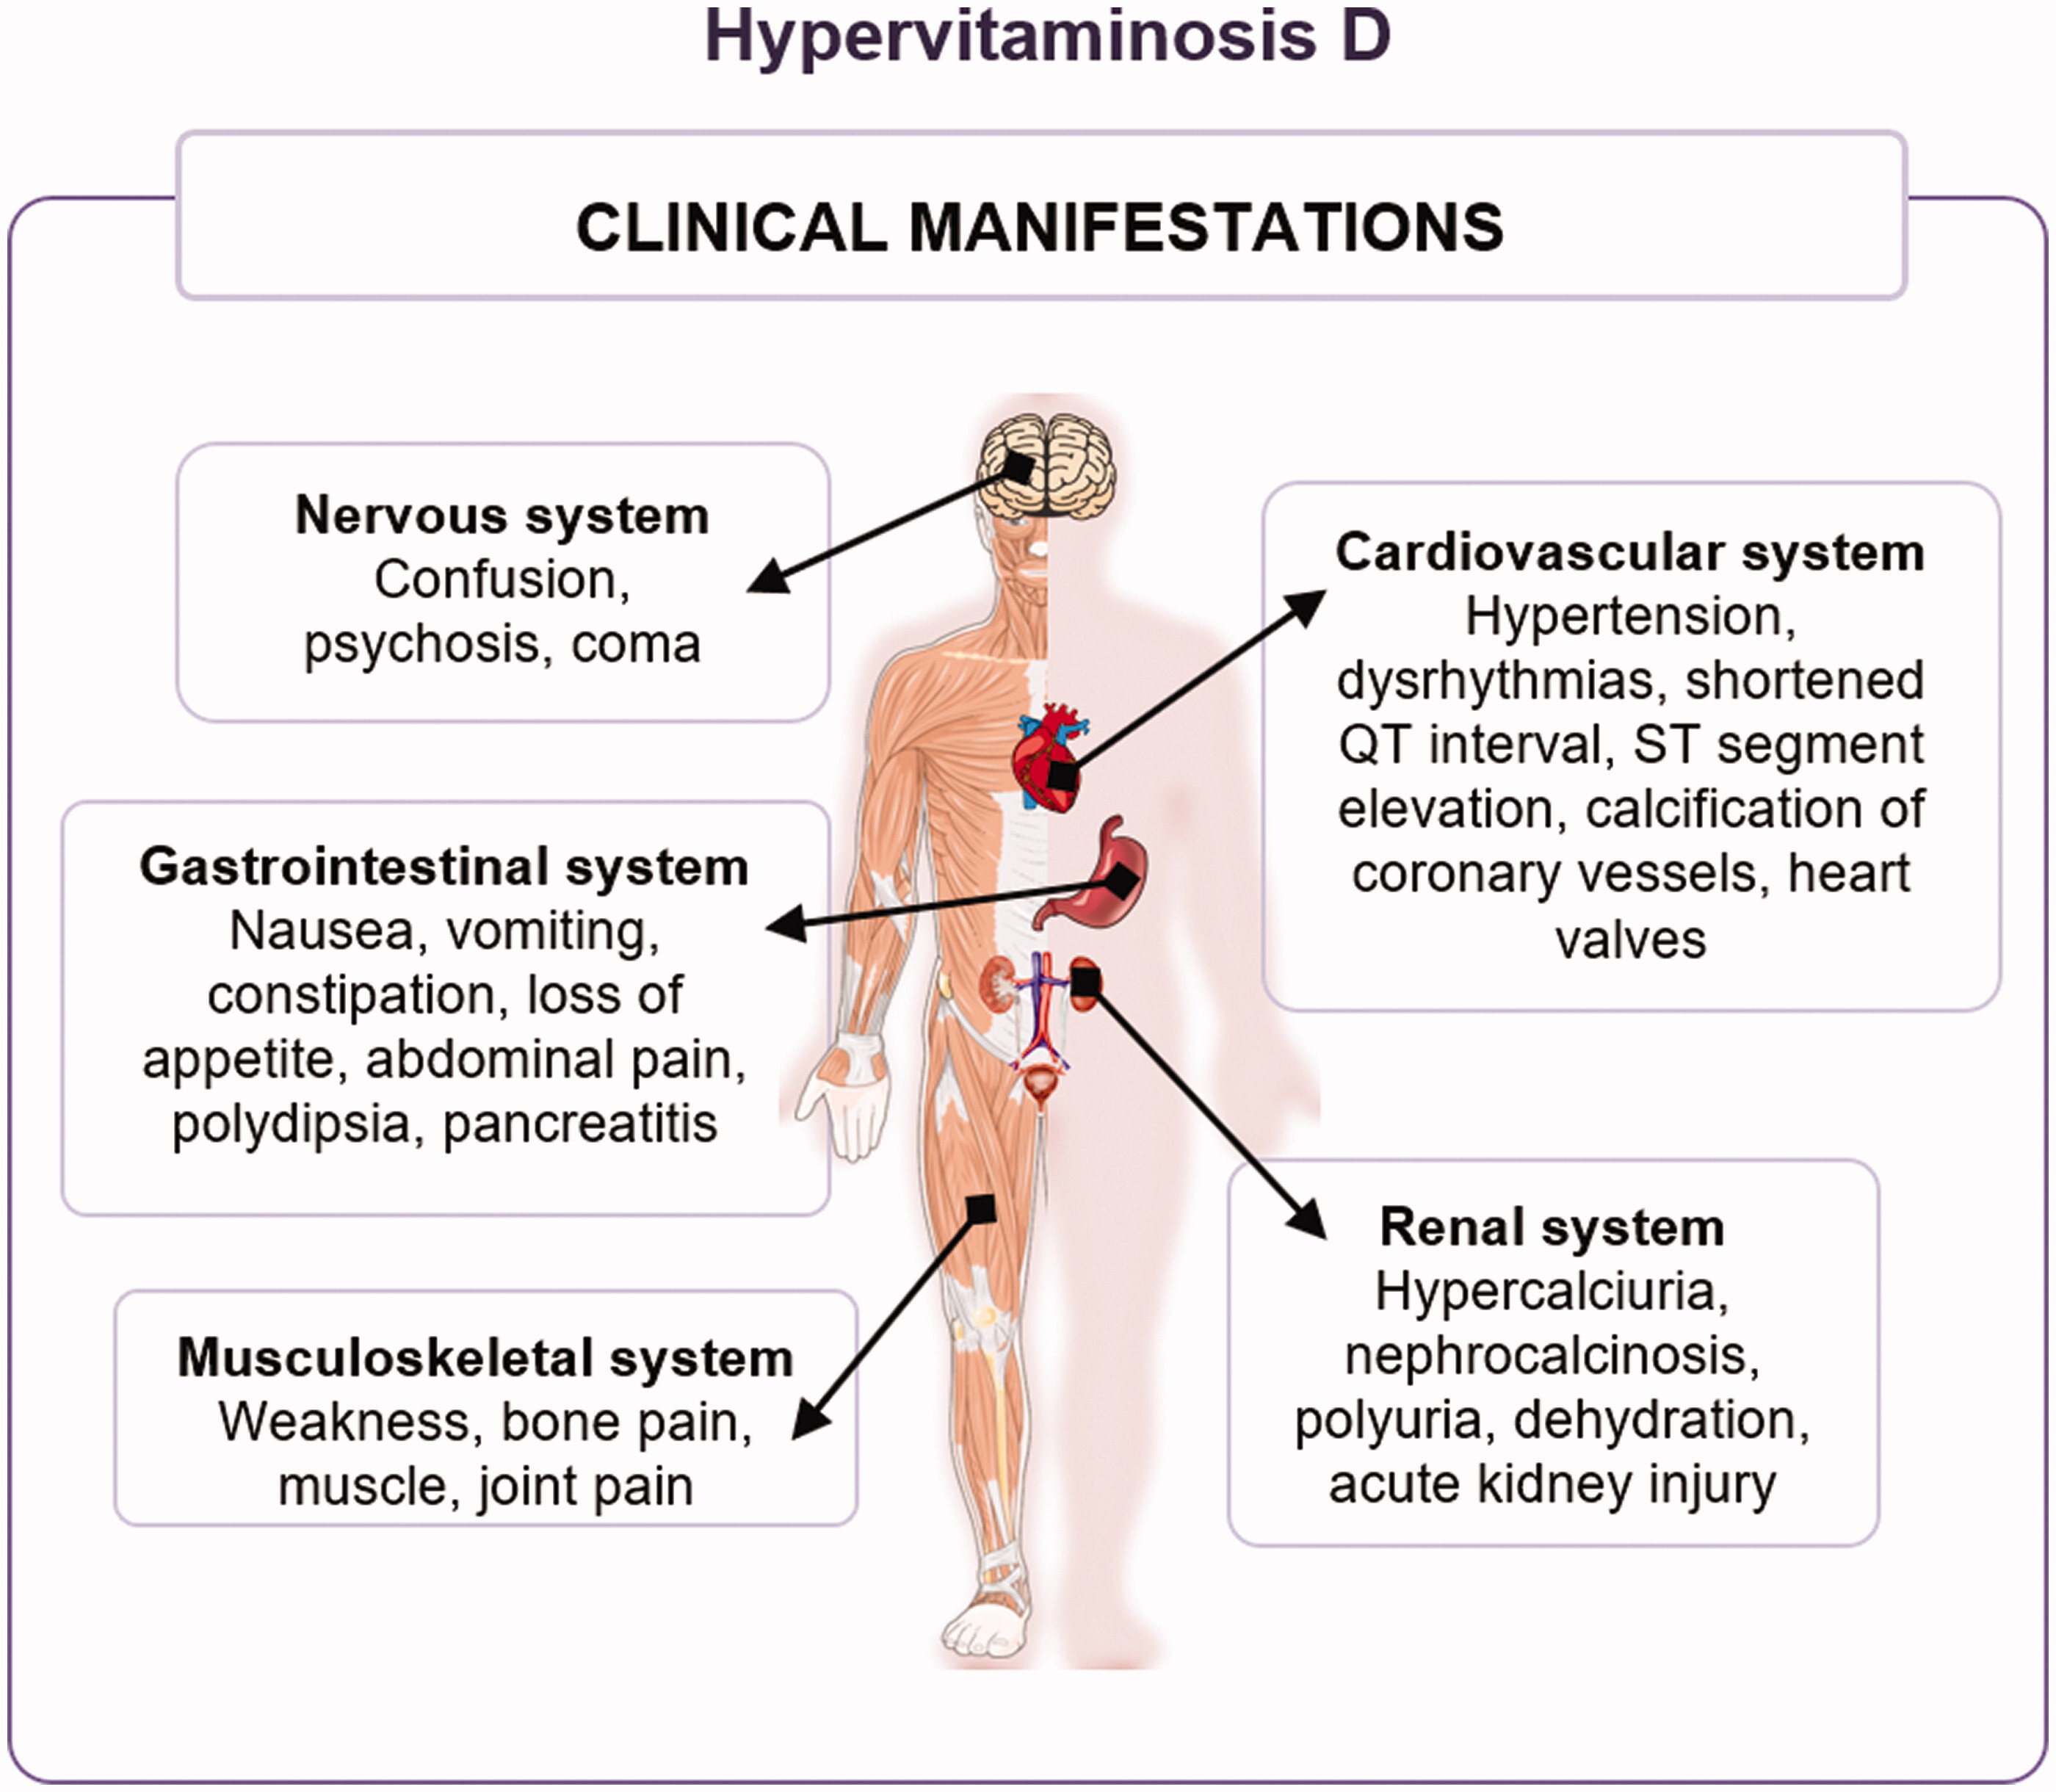
\includegraphics{figures/hypervitaminosis-d.jpg}

}

\caption[Symptômes associés lors d'une hypervitaminose
D.]{\label{fig-hypervitaminose-d}\textbf{Symptômes associés lors d'une
hypervitaminose D} \autocite{Janoušek.2022}.}

\end{figure}%

La toxicité de la vitamine D est habituellement d'origine iatrogène, le
surdosage de vitamine D pouvant être accidentel, conséquence d'une
erreur médicale ou d'un malentendu sur des recommandations médicales
\autocite{Lim.2020vd}. Elle peut aussi résulter d'une activité excessive
de la production endogène anormale de calcitriol par les macrophages
chez les patients lors de maladies granulomateuses comme la sarcoïdose,
les maladies fongiques, la lèpre et la bérylliose
\autocite{Marcinowska-Suchowierska.2018}. Il peut exister enfin des
situations d'excès de \ac{25(OH)D3} et de \ac{1,25(OH)2D3} dans des
troubles congénitaux, tels que le syndrome de Williams-Beuren, qui
s'accompagne d'une déficience en 24-hydroxylase, et donc ne permet pas
la métabolisation de \ac{25(OH)D3} and \ac{1,25(OH)2D3} en métabolites
inactifs \autocite{Marcinowska-Suchowierska.2018}. Ce syndrome cause
ainsi hypercalcémie, néphrolithiase, et néphrocalcinose
\autocite{Azer.2021}.

\subsection{Seuil de toxicité actuel}\label{seuil-de-toxicituxe9-actuel}

L'\ac{IOM} a fixé à 4000 UI/j de cholécalciférol la limite supérieure de
sécurité, c'est-à-dire la dose maximale pouvant être consommée sans
risque de façon chronique. Ce seuil a été établi en considérant un
apport de 10 000 UI/j de cholécalciférol comme le nouveau d'apport le
plus élevé non associé à des effets négatifs et en tenant compte des
incertitudes sur des données comme la mortalité toute causes, pour des
prises inférieures à 10 000 UI/j. La limite supérieure de sécurité
concerne également les enfants de 9 à 18 ans mais est réduite pour les
enfants de 1 à 8 ans (2500 à 3000 UI/j). Cependant l'IOM admet que les
signes de toxicité de la vitamine D sont rares pour une valeur de 10 000
UI/j, mais que la toxicité est plus commune vers des doses de 50 000
UI/j . Ces valeurs sont toutefois basées sur des données limitées et des
études supplémentaires sont nécessaires pour déterminer les effets de la
vitamine D sur la santé au-delà de ces valeurs \autocite{IOM.2011}.

L'ANSM a publié un avis sur le bon usage de la vitamine D, suite à des
cas rapportés de surdosage de vitamine D entraînant une hypercalcémie,
parfois accompagnée de lithiase et néphrocalcinose chez des enfants et
des nourrissons, après avoir pris une dose plus de deux fois supérieure
à la dose recommandée (400 UI par jour de 0 à 18 ans chez l'enfant en
bonne santé sans facteur de risque, 800 UI par jour de 0 à 18 ans chez
l'enfant présentant un facteur de risque) pendant plusieurs semaines, et
deux cas d'intoxication sévère à la vitamine D après avoir pris un
complément alimentaire acheté sur internet contenant une dose de 10 000
UI par goutte \autocite{ANSM.2021}.

--\textgreater{}

\newpage{}

\chapter{Vitamine D, système immunitaire et réponse
antivirale}\label{vitamine-d-systuxe8me-immunitaire-et-ruxe9ponse-antivirale}

L'importance du rôle de la vitamine D sur le système immunitaire a
récemment retenu l'attention des chercheurs depuis la découverte de la
coexistence du \ac{VDR} et du \ac{CYP27B1} dans des tissus dont la
fonction n'est pas directement liée à l'homéostasie du calcium
\autocite{Zehnder.2001}. En particulier, l'expression du \ac{CYP27B1}
dans les cellules immunitaires est régulée indépendamment de
l'homéostasie du calcium \autocite{White.2022}. Deux observations
principales suggèrent un rôle de la vitamine D dans le système
immunitaire : le \ac{VDR} est présent dans toutes les cellules
immunitaires, et la présence du \ac{CYP27B1} est induite par certaines
cellules immunes \autocite{Giannini.2022}. De ce fait, cette découverte
de la présence de CYP27B1 extra-rénale suggère un rôle local de l'action
paracrine ou intracrine du calcitriol
\autocite{Hewison.2007,Bishop.2021}.

La vitamine D agit à la fois sur le système immunitaire inné et
adaptatif (\Cref{fig-vd-immune-effect}). En effet, par le biais de la
synthèse intracrine du calcitriol par les macrophages et cellules
dendritiques, le calcitriol est active en amont et en aval des \acp{PRR}
qui jouent un rôle initial dans la réponse innée, stimule la production
de peptides antimicrobiens et en particulier la cathélicidine dont il
est un puissant inducteur, diminue les concentrations de fer via
l'induction de l'hepcidine, augmente l'autophagie permettant de
combattre les pathogènes intracellulaires tels que \emph{M.
tuberculosis} \autocite{Liu.2006}, et les infections virales, et joue un
rôle important dans le système adaptatif par une suppression des
réponses cellulaires \ac{Th1} et \ac{Th17} tout en promotant une
immunotolérance \autocite{Bishop.2021,Ismailova.2022}.

Ainsi, plusieurs cellules immunitaires peuvent synthétiser l'enzyme clé
permettant la conversion du \ac{25(OH)D3} en \ac{1,25(OH)2D3}, le
cytochrome \ac{CYP27B1} ou aussi appelée 1α-hydroxylase. L'induction de
cette enzyme concerne des cellules telles que les cellules dendritiques,
monocytes, macrophages, lymphocytes B et T
\autocite{Giannini.2022,Dankers.2017}.

Dans ce contexte, l'enzyme 1α-hydroxylase n'est pas uprégulée par la
\ac{PTH}. Par conséquent, la production de \ac{1,25(OH)2D3} dépend des
niveaux de substrat de \ac{25(OH)D3} et peut être régulée par des
signaux inflammatoires, tels que le \ac{LPS} et les cytokines
\autocite{Giannini.2022}.

\section{Mécanismes d'action de la vitamine D sur le système
immunitaire}\label{muxe9canismes-daction-de-la-vitamine-d-sur-le-systuxe8me-immunitaire}

Comme nous allons le voir, la vitamine D possède une action globalement
anti-inflammatoire et donc régulatrice de l'inflammation
(\Cref{fig-vd-immune-effect}). Elle agit à la fois sur le système
immunitaire inné et adaptatif. A l'initiation de la réponse
inflammatoire, le calcitriol est essentiel afin de répondre à une
infection. Les effets de la vitamine D ne répriment pas totalement le
système immunitaire mais plutôt induit une modulation immunitaire, en
faisant évoluer le système immunitaire adaptatif vers une tolérance
antigénique, et le système immunitaire inné vers une meilleure
élimination virale et bactérienne \autocite{Martens.2020}. Le calcitriol
n'est donc pas purement anti-inflammatoire mais il contribue à maintenir
l'équilibre entre un état pro- et anti-inflammatoire et est donc capable
de rétablir l'équilibre perturbé \autocite{Dankers.2017}.

\begin{figure}

\centering{

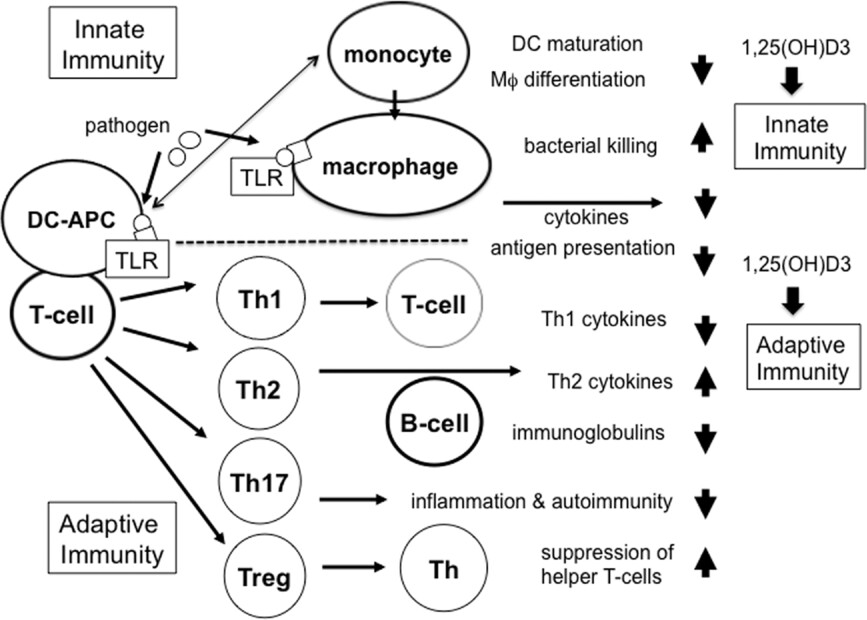
\includegraphics{figures/vd-immune-effect.jpg}

}

\caption[Effets du calcitriol sur la réponse
immunitaire.]{\label{fig-vd-immune-effect}\textbf{Effets du calcitriol
sur la réponse immunitaire.} La \ac{1,25(OH)2D3} régule à la fois
l'immunité innée et l'immunité adaptative, en potentialisant l'activité
antimicrobienne des macrophages, en diminuant la présentation de
l'antigène et en diminuant les fonctions des lymphocytes B et de
certains lymphocytes T. Cependant, dans des conditions normales, le
\ac{1,25(OH)2D3} augmente le phénotype \ac{Th2} et l'efficacité des
\ac{Treg}. DC, cellules dendritiques. \autocite{Cutolo.2014}}

\end{figure}%

\subsection{Action intracrine et
autocrine}\label{action-intracrine-et-autocrine}

Les études suggèrent que la vitamine D délivre ses effets par un
mécanisme intracrine ou autocrine et non systémique au sein des tissus
non-classiques \autocite{Hewison.2007} et agit localement dans les
cellules immunitaires. Un mécanisme intracrine se réfère à un mécanisme
impliquant une molécule agissant et produite par la même cellule. En
effet, trois aspects spécifiques de la \ac{CYP27B1} ont attiré
l'attention des chercheurs : l'expression et la régulation dans les
tissus non classiques au cours de la physiologie normale ; les effets
sur le système immunitaire et les maladies inflammatoires ; l'expression
et la fonction dans les tumeurs.

\textcite{Hewison.2007} investigue l'idée d'un mécanisme extra-rénal de
\ac{CYP27B1} rapporté dans la littérature et l'efficacité de la réponse
du calcitriol endogène dans la modulation de la réponse immune. En
représentant les conditions de carence en vitamine D, d'insuffisance en
vitamine D et de suffisance en vitamine D, par une dose de 5, 50 and 150
nM de calcidiol respectivement et d'un inhibiteur de CYP27B1,
l'accumulation de calcitriol dans les cellules dendritiques et
macrophages est due à l'activité de l'enzyme 1α-hydroxylase et est
augmenté lorsque les concentrations de calcidiol augmentent, et impacte
selon une relation dose-dépendante la stimulation de CD14 et la
répression de marqueurs de cellule dendritique CD86, CD83 et HLA-DR.

Similairement, l'essai \emph{in vitro} de \textcite{Adams.2009} montre
que le calcidiol est nécessaire pour produire la cathélicidine, un
peptide antimicrobien, et qu'elle est dépendante de l'expression du
\ac{CYP27B1} du macrophage, bien qu'à haute concentration le calcidiol
peut stimuler la production de cathélicidine sans passer par
l'activation des macrophages via le \ac{TLR} De plus, l'expression de
cathélicidine est notablement diminuée lorsque la concentration de
vitamine D administrée est inférieure à 30 ng/mL. En outre, les auteurs
ont observé une absence de corrélation entre les niveaux de
cathélicidine plasmatique et les niveaux de calcidiol plasmatique, ainsi
que la concentration de cathélicidine leucocytaire et la concentration
plasmatique de calcidiol, ce qui suggère que l'effet de la vitamine D
sur la synthèse de la cathélicidine par les cellules immunes est due non
pas à la présence de calcidiol plasmatique mais bien à l'effet local
intracrine des cellules immunes.

De même, \textcite{Zhang.2012} a montré que la vitamine D inhibe la
production de cytokine dans des monocytes, et que l'effet n'est observé
uniquement lorsque la concentration est supérieure ou égale à 30 ng/mL
de calcidiol et 0,04 ng/mL de calcitriol. La vitamine D inhibe la
production de IL-6 et \ac{tnfa}, normalement induite par le \ac{LPS}. Ce
mécanisme passe par l'activation de la MKP-1, la mitogen-activated
protein kinase-phosphatase 1 qui désactive la production de cytokine.

L'effet autocrine de la vitamine D sur des lymphocytes T
CD4\textsuperscript{+} a été observé par \textcite{Chauss.2022}.
L'administration de calcitriol actif ou calcidiol conduit aux cellules à
réprimer l'\ac{ifng} et augmenter la synthèse d'\ac{IL-10}, indiquant
que les cellules ont acquises la capacité de métaboliser et de répondre
aux métabolites de la vitamine D. Inversement, lors du KO d'un des gènes
concernant la vitamine D tel que \emph{CTSL}, \emph{VDR} ou
\emph{CYP27B1}, une réduction nette en \ac{IL-10} est observée. Dans
l'ensemble les résultats indiquent l'effet d'un mécanisme
intracellulaire autocrine/paracrine de la vitamine D. Des résultats
similaires ont été retrouvé par \textcite{Adams.2009} par le KO du
\emph{VDR} et \emph{CYP27B1} et l'expression de la cathélicidine
diminuée.

\subsection{Induction de l'immunité innée
antimicrobienne}\label{induction-de-limmunituxe9-innuxe9e-antimicrobienne}

Après l'entrée du calcitriol dans la cellule ou la conversion du
calcidiol en calcitriol intracellulaire, l'action du calcitriol est
médié par l'hétérodimère \ac{VDR}-\ac{RXR} et se fixe sur le \ac{VDRE},
causant la régulation de multiples gènes
(\Cref{fig-vd-immune-signaling}) \autocite{Caprio.2017,Yasmin.2005}. Un
des mécanismes principaux de l'immunité innée antimicrobienne passe par
l'induction de peptides antimicrobiens et en particulier la forte
induction de cathélicidine \autocite{Wang.2004}. En effet, la vitamine D
stimule l'expression du gène \emph{CAMP} en se liant au \ac{VDRE} situé
son promoteur et induit la cathélicidine humaine hCAP-18, clivant ce
précurseur en LL-37 par la protéinase 3. Le domaine C-terminal de hCAP18
nommé LL-37, est un peptide antimicrobien qui déstabilise les membranes
bactériennes et fongiques et peut empêcher la réplication virale en se
liant aux protéines de pointes \autocite{Bishop.2021,Charoenngam.2020}.
De plus, LL-37 est impliqué dans la signalisation, induisant la
chimiotaxie et participe à la régénération tissulaire et est capable
d'activer les TLR7 et TLR8 activant la cellule dendritique
\autocite{Silva.2012}. Le LL-37 est exprimé par les leucocytes,
notamment les neutrophiles, les monocytes, les mastocytes, les cellules
NK, les lymphocytes T et B. Le LL-37 a également été trouvé dans le
plasma, la moelle osseuse, les voies respiratoires, l'intestin, les
glandes mammaires, l'épididyme et la peau \autocite{Silva.2012}. De
plus, le calcitriol induit également le peptide antimicrobien défensine
\mupbeta 2 via le gène \emph{HBD2}, où la combinaison du IL-1\mupbeta et
du calcitriol augmente l'induction de \emph{HBD2}
{[}\textcite{Bishop.2021}; Wang.2004{]}.

\begin{figure}

\centering{

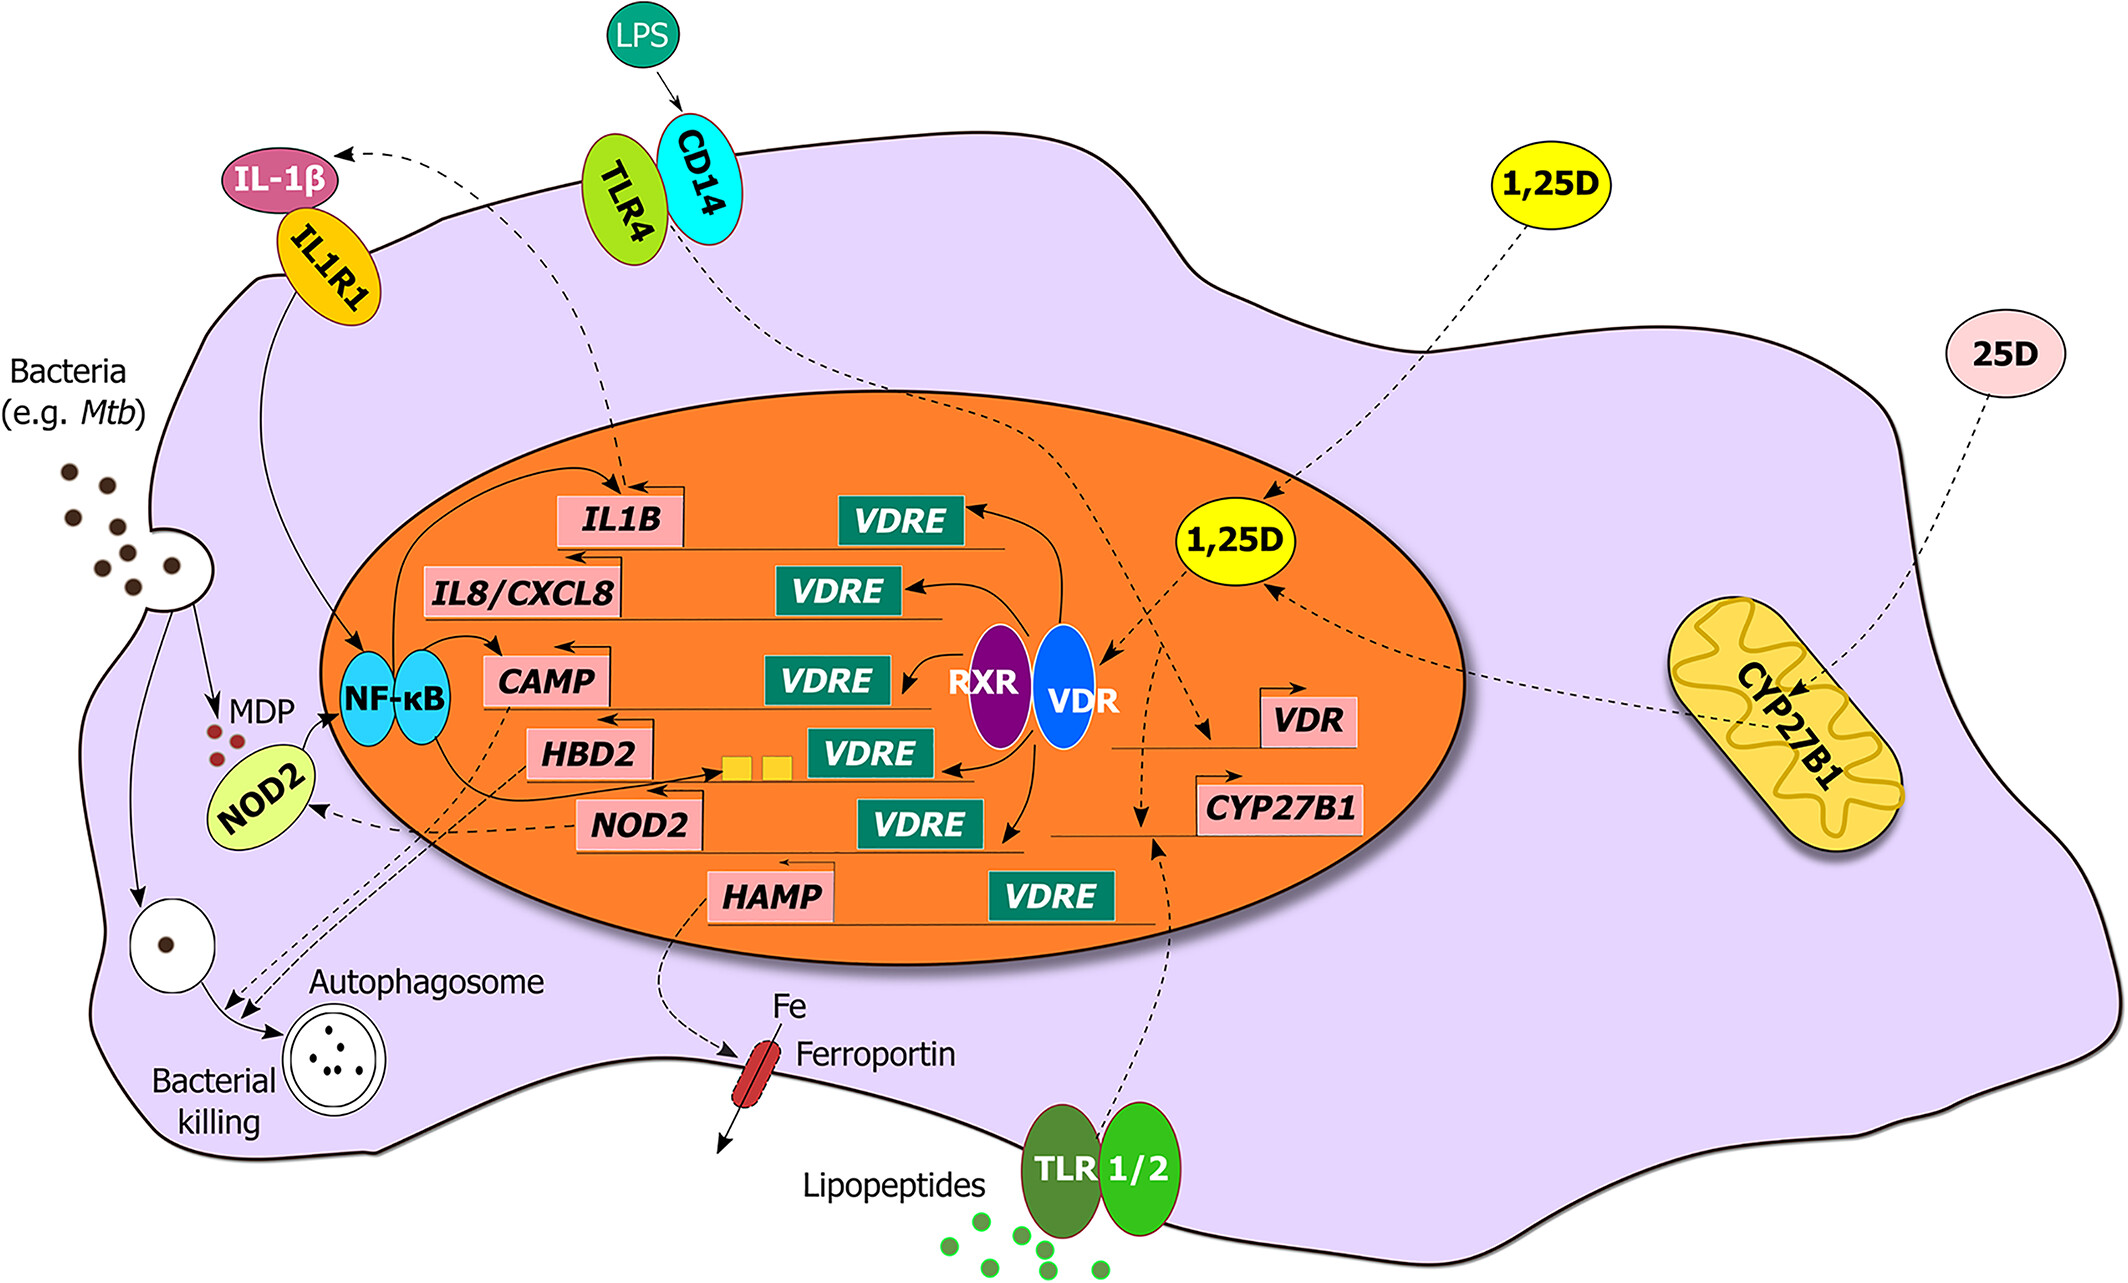
\includegraphics{figures/Bishop.2021-Vitamin_D_metabolism_and_innate_immune_signaling_in_the_monocyte-macrophage.jpg}

}

\caption[Métabolisme de la vitamine D et signalisation immunitaire innée
dans le
monocyte/macrophage.]{\label{fig-vd-immune-signaling}\textbf{Métabolisme
de la vitamine D et signalisation immunitaire innée dans le
monocyte/macrophage.} Après liaison du calcitriol sur le \ac{VDR}, le
complexe \ac{VDR}-\ac{RXR} se lie sur différentes séquences \ac{VDRE}
spécifiques, induisant l'expression de peptides antimicrobiens tel que
la cathélicidine et la défensine \mupbeta 2, diminue l'expression de
l'hepcidine, favorise l'autophagie, l'expression de \ac{PRR} comme NOD2
et de cytokines tel que l'IL-8 et l'IL-1β. \autocite{Bishop.2021}.}

\end{figure}%

Le calcitriol régule en outre négativement l'expression d'un agent
antibactérien, la protéine antibactérienne hepcidine en réprimant le
gène \emph{HAMP}, qui a pour fonction de réduire l'exportation du fer
médiée par la ferroportine. En effet, presque tous les microorganismes
utilisent le fer pour leur croissance. De ce fait, la restriction du fer
par l'organisme constitue une des réponses afin de lutter contre
l'infection ; l'expression de l'hepcidine est augmentée lors de stimuli
bactériens et viraux \autocite{Bishop.2021}. La régulation négative de
l'hepcidine par le calcitriol facilite l'exportation du fer et diminue
la concentration intracellulaire de fer.

Un autre aspect de la régulation du calcitriol concerne la régulation de
l'expression de \ac{PRR}. En effet le calcitriol induit le \ac{PRR}
\acl{NOD}-2 (\acsu{NOD}2) qui reconnaît le \ac{MDP} généré par la
décomposition du peptidoglycane bactérien. De manière manière dépendante
au \ac{nfkb}, NOD2 induit l'expression de la défensine \mupbeta 2 et de
la cathélicidine (\Cref{fig-vd-immune-signaling})
\autocite{Bishop.2021,Ismailova.2022}.

De plus, le calcitriol induit l'autophagie par de multiples voies :
indirectement, la reconnaissance du \ac{MDP} par NOD2 favorise
l'autophagie \autocite{Bishop.2021}, la cathélicidine agit sur des gènes
liés à l'autophagie \autocite{Yuk.2009}, et la présence de calcitriol
est capable d'induire plus directement l'autophagie, où la présence
d'analogue de calcitriol a montré une inhibition de mTOR, une protéine
régulatrice de l'autophagie \autocite{Yuk.2009}. L'autophagie est un
processus de dégradation des protéines et des organites endommagés, et
est un mécanisme de défense contre les infections virales et
bactériennes, en particulier les infections intracellulaires telles que
\emph{M. tuberculosis} \autocite{Liu.2006}.

\subsection{Effets immunomodulateurs}\label{sec-immunomodulateur}

Bien que la vitamine D possède principalement un effet activateur du
système immunitaire inné, elle possède globalement un effet
immunorégulateur du système immunitaire adaptatif, en particulier
concernant les lymphocytes T et B \autocite{Bishop.2021}. Les
lymphocytes T sont impliqués dans la reconnaissance des antigènes et la
destruction des cellules infectées ou tumorales, tandis que les
lymphocytes B sont impliqués dans la production d'anticorps. La vitamine
D agit sur ces deux types de lymphocytes en modulant leur fonctionnement
et leur activation (\Cref{fig-vd-immune-effect}).

\subsubsection{Macrophages, monocytes et
neutrophiles}\label{macrophages-monocytes-et-neutrophiles}

Comme discuté précédemment, les effets du calcitriol ne sont pas
toujours de nature pro-inflammatoire. La vitamine D possède un pouvoir
pro-inflammatoire dans la réponse initiale de l'inflammation, puis un
pouvoir anti-inflammatoire lors de la phase de résolution de
l'inflammation \autocite{Dankers.2017}. En effet, la culture de
monocytes avec le \ac{LPS} montre une répression de l'\ac{IL-10} pendant
les 8 premières heures, suivie d'une induction de l'IL-10 48 heures
après la réponse initiale \autocite{Matilainen.2010}.

Le calcitriol induit le switch phénotypique de macrophage M1 vers M2 par
la régulation positive de l'\ac{IL-10}. Le macrophage M2 est un type de
macrophage ayant un profil anti-inflammatoire contrairement au
macrophage M1 au profil pro-inflammatoire. Le calcitriol inhibe
également des cytokines majeures pro-inflammatoires telles que
l'\ac{IL-6} et le \ac{tnfa}, et l'action du \ac{nfkb}
\autocite{Meza-Meza.2022,Caprio.2017}. Il a également été démontré que
le calcitriol supprime l'expression des \ac{TLR}2 et \ac{TLR}4 et induit
le CD14 sur les monocytes \autocite{Bishop.2021} et inhibe la production
des cytokines inflammatoires \ac{IL-2}, l'\ac{IL-6} et l'\ac{IL-17}
\autocite{Meza-Meza.2022,Caprio.2017}.

Le calcitriol induit robustement l'IL-8 \autocite{Bishop.2021}, qui
recrute les neutrophiles tout comme l'IL-1\mupbeta ~sur le lieu de
l'inflammation, et augmente à son tour la production de IL-8 par les
neutrophiles. Cependant il est rapporté que le pouvoir phagocytique du
macrophage est diminué, mais n'affecte pas celui du neutrophile
\autocite{Chen.2017}.

\begin{figure}

\centering{

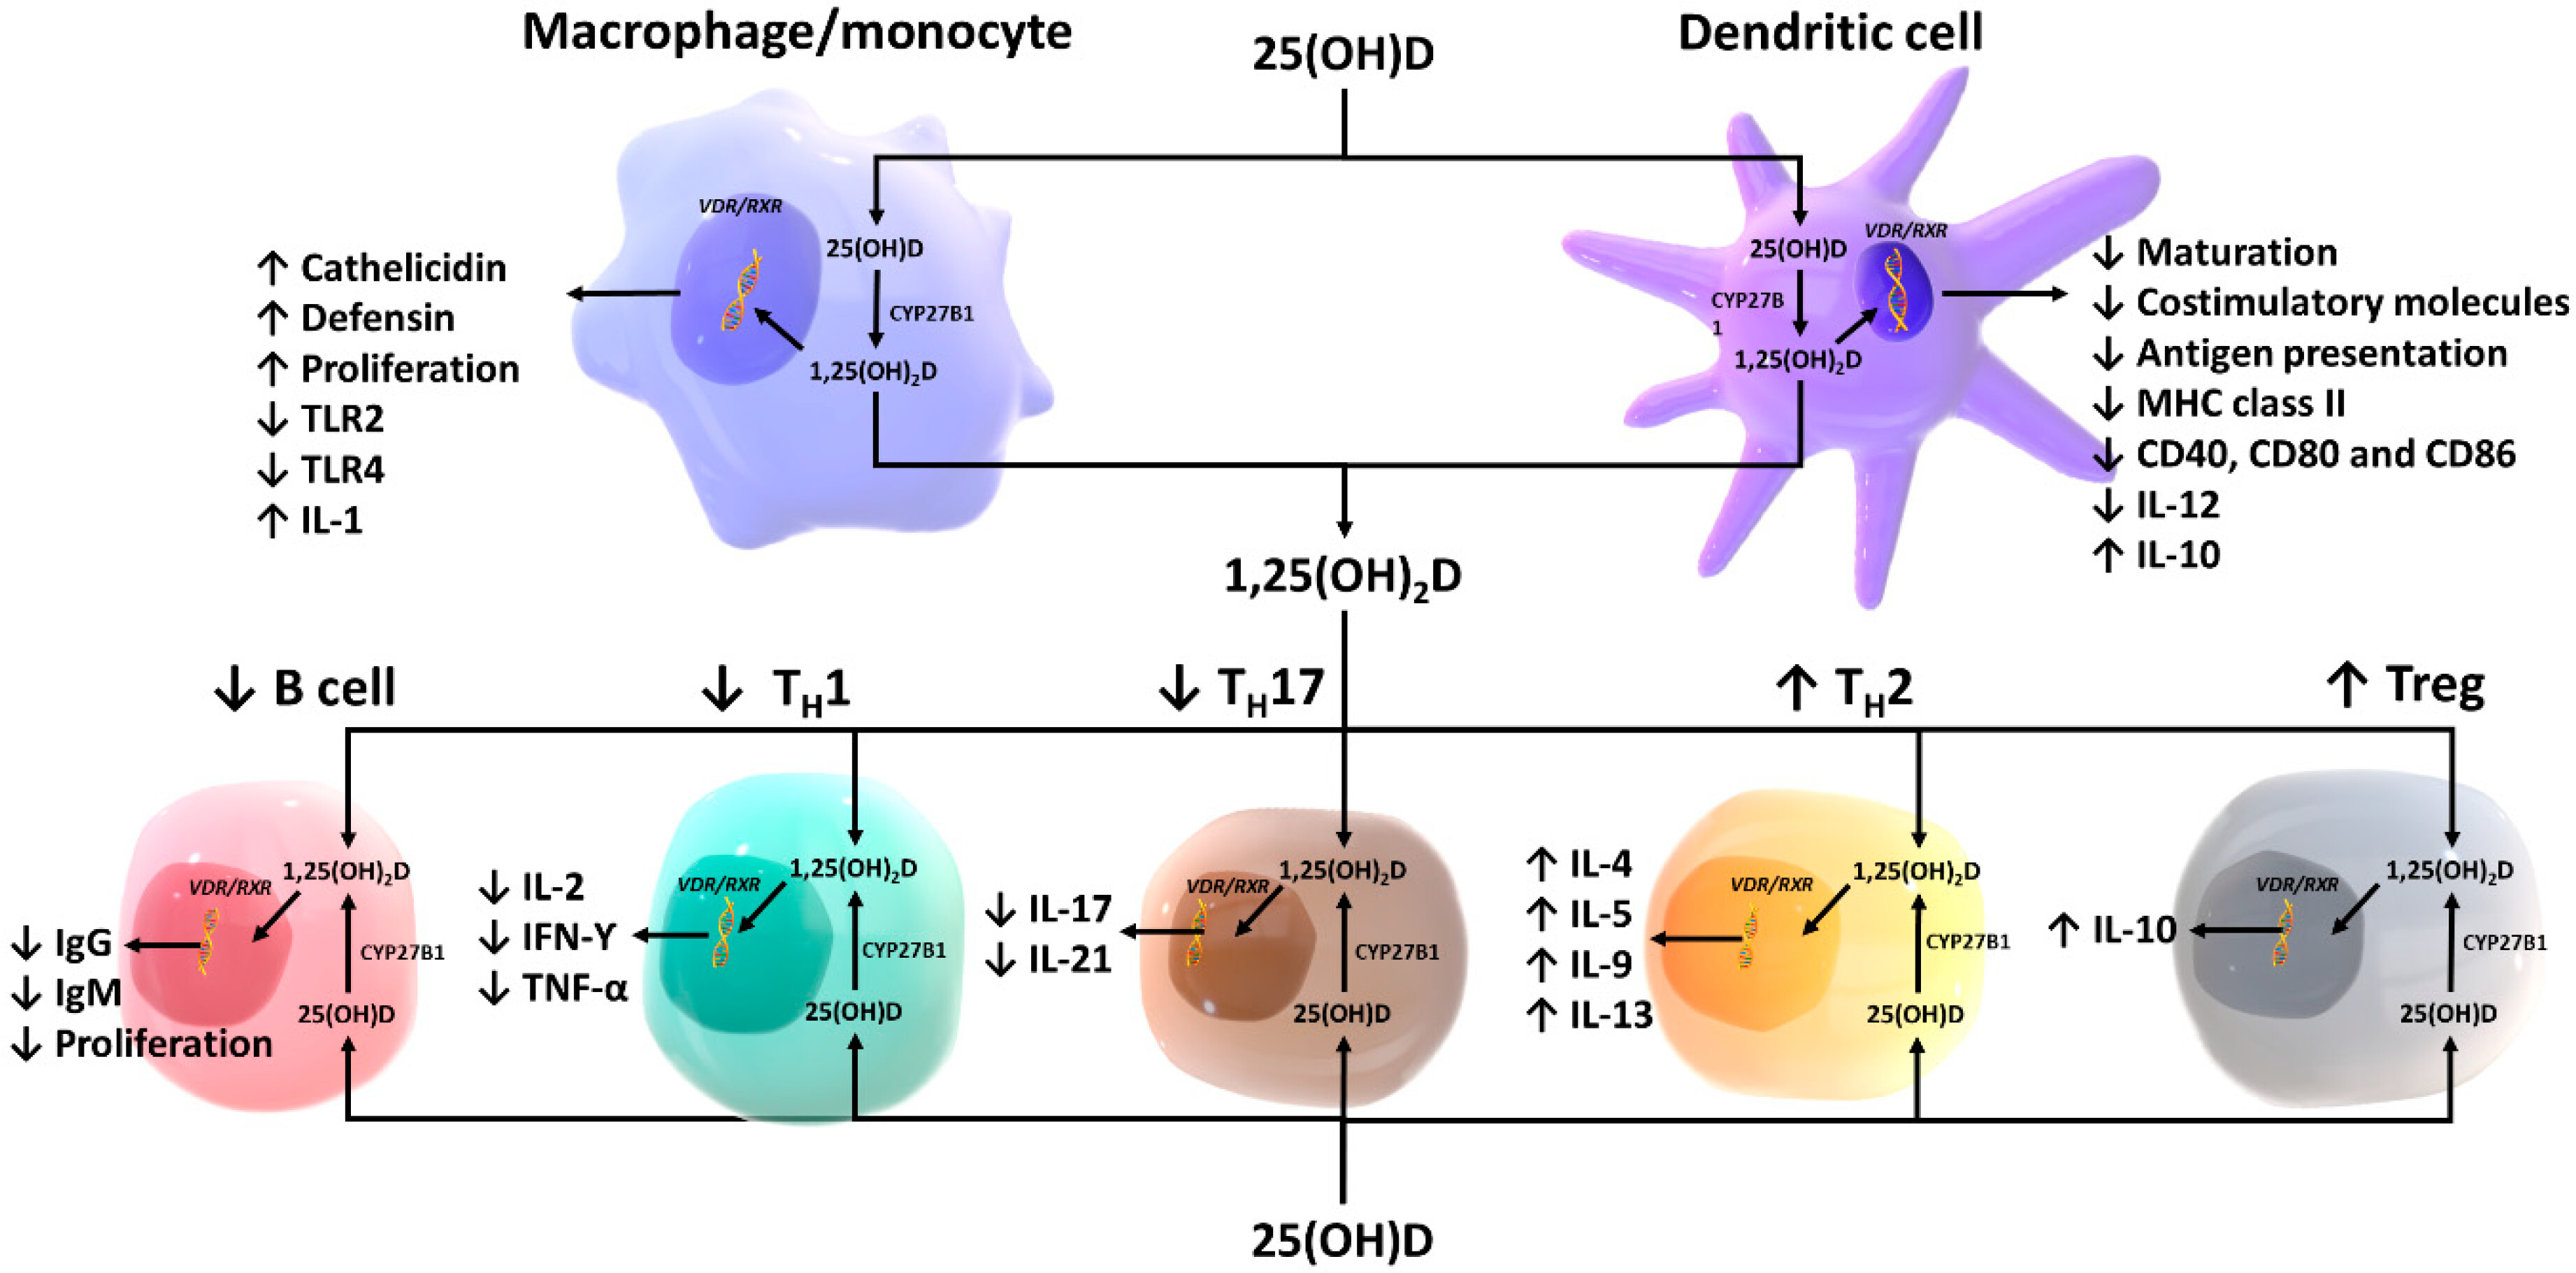
\includegraphics{figures/vd-action.jpg}

}

\caption[Représentation schématique des fonctions paracrine et
intracrine de la vitamine D et de ses métabolites et des actions de la
\ac{1,25(OH)2D3} sur les systèmes immunitaires innés et
adaptatifs.]{\label{fig-vd-action}\textbf{Représentation schématique des
fonctions paracrine et intracrine de la vitamine D et de ses métabolites
et des actions de la \ac{1,25(OH)2D3} sur les systèmes immunitaires
innés et adaptatifs.} Les macrophages, monocytes et cellules
dendritiques sont capables d'induire le \ac{CYP27B1} afin de métaboliser
le calcidiol en calcitriol, qui va ensuite agir de manière intracrine
par le biais de la translocation de l'hétérodimère \ac{VDR}-\ac{RXR} et
agir directement sur l'expression des facteurs de transcription.
Globalement les effets issus du calcitriol seront liés à l'augmentation
de la défense innée notamment par le biais de la cathélicidine, ainsi
qu'une diminution du phénotype mature de la cellule dendritique et une
augmentation du phénotype tolérogène. Par la suite, le calcitriol peut
agir sur les cellules environnantes en favorisant un phénotype
anti-inflammatoire chez les cellules \ac{Th2} et \ac{Treg} ainsi qu'une
diminution de l'activation des cellules \ac{Th1} et \ac{Th17}, et des
cellules B. \autocite{Charoenngam.2020}}

\end{figure}%

\subsubsection{Lymphocytes NK}\label{lymphocytes-nk}

Les cellules \ac{NK} sont des lymphocytes qui jouent un rôle important
dans l'immunité innée en éliminant les cellules infectées par un virus
ou les cellules tumorales. Certains sous-types de lymphocytes NK
possèdent un rôle peu cytotoxique mais produisent des cytokines en
abondance tandis que le sous-type cytotoxique est caractérisé par
l'exocytose de granzymes et perforines \autocite{Moretta.2008}. Le
calcitriol contribue à augmenter le pouvoir cytotoxique des lymphocytes
\ac{NK}, régule la production de cytokines, induit l'expression de
sous-type NK régulateur IL-10\textsuperscript{+}, mais n'a pas
d'incidence sur la prolifération des \ac{NK}.

En outre, des études expérimentales ont suggéré que la différenciation
et la fonction des lymphocytes \ac{NK} peuvent être modulées par un
traitement au calcitriol \autocite{Charoenngam.2020}. Cependant, le rôle
inducteur ou inhibiteur du calcitriol est encore indéterminé par manque
de données cohérentes.

\subsubsection{Cellules présentatrices
d'antigènes}\label{cellules-pruxe9sentatrices-dantiguxe8nes}

Le calcitriol agit également sur les \ac{CPA} : cellules dendritiques,
macrophages, lymphocytes B, par le biais d'une diminution de
l'expression de \ac{CMH-II} qui leur permet de présenter des antigènes
étrangers, ainsi que l'expression de molécules de co-stimulation
(\ac{CD} 40, CD80, CD86) qui contribue à la signalisation positive ou
négative lors de la reconnaissance du complexe CMH-peptide par le
\ac{TCR} et conduit l'activation des lymphocytes T lors de la
présentation antigénique par les \ac{CPA}. (\Cref{fig-vd-action})
\autocite{Charoenngam.2020,Meza-Meza.2022,Caprio.2017}. Ce changement
phénotypique s'accompagne donc d'une diminution de la capacité de
présentation d'antigènes et de production d'\ac{IL-12}, interleukine clé
pour la différenciation des lymphocytes T en Th1 et lymphocytes
CD8\textsuperscript{+}, ainsi qu'une augmentation d'\ac{IL-10} produite.

La cellule dendritique en particulier acquiert un phénotype tolérogène
spécifique par l'induction du calcitriol (\Cref{fig-immunomod}), avec
une baisse du pouvoir de présentation antigénique et de stimulation, et
une augmentation de la synthèse de cytokines anti-inflammatoires et en
particulier l'IL-10 \autocite{Bishop.2021}.

L'IL-10 est la cytokine majeure par laquelle sont activés les \ac{Treg}
et médient leurs actions. Elle a des effets immunosuppresseurs
significatifs sur les monocytes, les macrophages et les cellules
dendritiques, qui expriment le récepteur à l'IL-10. Elle inhibe la
production de cytokines et de chimiokines pro-inflammatoires et leur
différenciation, leur maturation et leur migration vers les organes
lymphoïdes. L'IL-10 réduit également les capacités de présentation de
l'antigène des monocytes et des \ac{CPA}. En outre, elle supprime
l'activation, la prolifération, la sécrétion de cytokines et l'activité
cytotoxique des lymphocytes T CD4\textsuperscript{+}, induisant une
anergie à long terme. Ainsi, l'IL-10 est une des cytokines maître de la
régulation de la réponse inflammatoire inflammatoire et favorise la
tolérance périphérique.

\subsubsection{Lymphocytes T}\label{lymphocytes-t}

Les lymphocytes T sont composés en plusieurs sous-groupes :

\begin{itemize}
\item
  les lymphocytes T auxiliaires ou helper CD4\textsuperscript{+} Th1,
  Th2, Th17. Les populations \ac{Th1} et \ac{Th17} ont principalement
  pour rôle de stimuler une réponse cytotoxique, respectivement
  intracellulaire antibactérienne et antiprotozoaire comme le
  toxoplasme, et extracellulaire antibactérienne et fongique. La
  population \ac{Th2} en revanche est centrée sur une stimulation de la
  réponse humorale ou médiée par les anticorps, contre les parasites
  extracellulaires, les bactéries, les allergènes et les toxines, médiée
  par le biais de cytokines causant une forte production d'anticorps,
  l'activation des éosinophiles et de l'inhibition de plusieurs
  fonctions des macrophages \autocite{Cantorna.2015,Walker.2018}
\item
  les lymphocytes T effecteurs CD8\textsuperscript{+} capables d'induire
  la mort des cellules.
\item
  les lymphocytes T CD4\textsuperscript{+} régulateurs ou \ac{Treg}, qui
  ont pour rôle de réguler l'inflammation et donc la réponse
  immunitaire.
\end{itemize}

Le calcitriol est capable d'induire le changement phénotypique des
sous-populations de lymphocytes T CD4+, favorisant le phénotype Th2, au
détriment des \ac{Th1} et \ac{Th17}, et l'expression des cytokines
\ac{Th2} (\Cref{fig-immunomod}). La sous-population \ac{Th2} réprime à
son tour les populations \ac{Th1} et \ac{Th17}, diminuant ainsi
globalement l'activité cytotoxique médiée par ces cellules
\autocite{Meza-Meza.2022}. De plus, le calcitriol inhibe la
prolifération des lymphocytes Th1 et Th17 \autocite{Cantorna.2015}.

Concernant les lymphocytes T CD8\textsuperscript{+}, la vitamine D
modifie un ratio bas de CD4/CD8 reflétant une activation immunitaire
plus forte à un ratio plus élevé de CD4/CD8, impliquant une suppression
immunitaire \autocite{Charoenngam.2020}. Le calcitriol diminue ainsi la
prolifération et l'hyperactivation des CD8\textsuperscript{+}, et la
sécrétion de \ac{ifng} et \ac{tnfa} par les CD8\textsuperscript{+}
activés \autocite{Dankers.2017}.

Le calcitriol est capable de promouvoir la différenciation des
CD4\textsuperscript{+} naïfs en \ac{Treg}, en partie indirectement grâce
au phénotype tolérogène des cellules dendritiques induit par le
calcitriol qui augmente la synthèse en IL-10, ainsi que l'induction d'un
phénotype \ac{Treg} à partir des Th1 et Th17. L'effet direct du
calcitriol sur les \ac{Treg} est peu clair, puisque les \ac{Treg}
expriment peu de \ac{VDR} et n'augmentent que peu ou pas la production
d'IL-10 en réponse au calcitriol \autocite{Bishop.2021}.

De ce fait, la présence de calcitriol est importante pour la suppression
de l'inflammation et la tolérance immunitaire.

\subsubsection{Lymphocytes B}\label{lymphocytes-b}

Le calcitriol exerce un rôle immunomodulateur sur les lymphocytes B
hyperactivés, exprimant le \ac{VDR} et le \ac{CYP27B1}. Le lymphocyte B
naïf, avant de devenir un plasmocyte sécréteur d'anticorps, nécessite de
se différencier en passant par la commutation de classe isotypique
(changement de classe d'anticorps) et l'hypermutation somatique
(augmentation de l'affinité des anticorps). Le calcitriol inhibe la
prolifération, induit l'apoptose et inhibe la commutation de classe
isotypique des lymphocytes B activés et plasmocytes
(\Cref{fig-immunomod}). En effet le mécanisme passe par l'inhibition du
\ac{nfkb}, qui aura pour conséquence de diminuer la signalisation
normale du CD40, le corécepteur du récepteur au lymphocyte B, où la
signalisation permet la différenciation des lymphocytes B
\autocite{Dankers.2017,Meza-Meza.2022}.

De plus, le \ac{VDR} est capable de se lier sur le promoteur du gène
exprimant l'IL-10, induisant une augmentation de la synthèse d'IL-10
\autocite{Dankers.2017,Martens.2020,Meza-Meza.2022}.

Le calcitriol réduit aussi le pouvoir présentateur des lymphocytes B par
la régulation à la baisse du CD86 et l'induction du CD74, qui permettent
de lier respectivement le CD28 et et le ligand \ac{MIF} situé sur le
lymphocyte T, supportant leur activation lorsque le lymphocyte B joue
son rôle de présentateur d'antigènes
\autocite{Dankers.2017,Martens.2020}.

\begin{figure}

\centering{

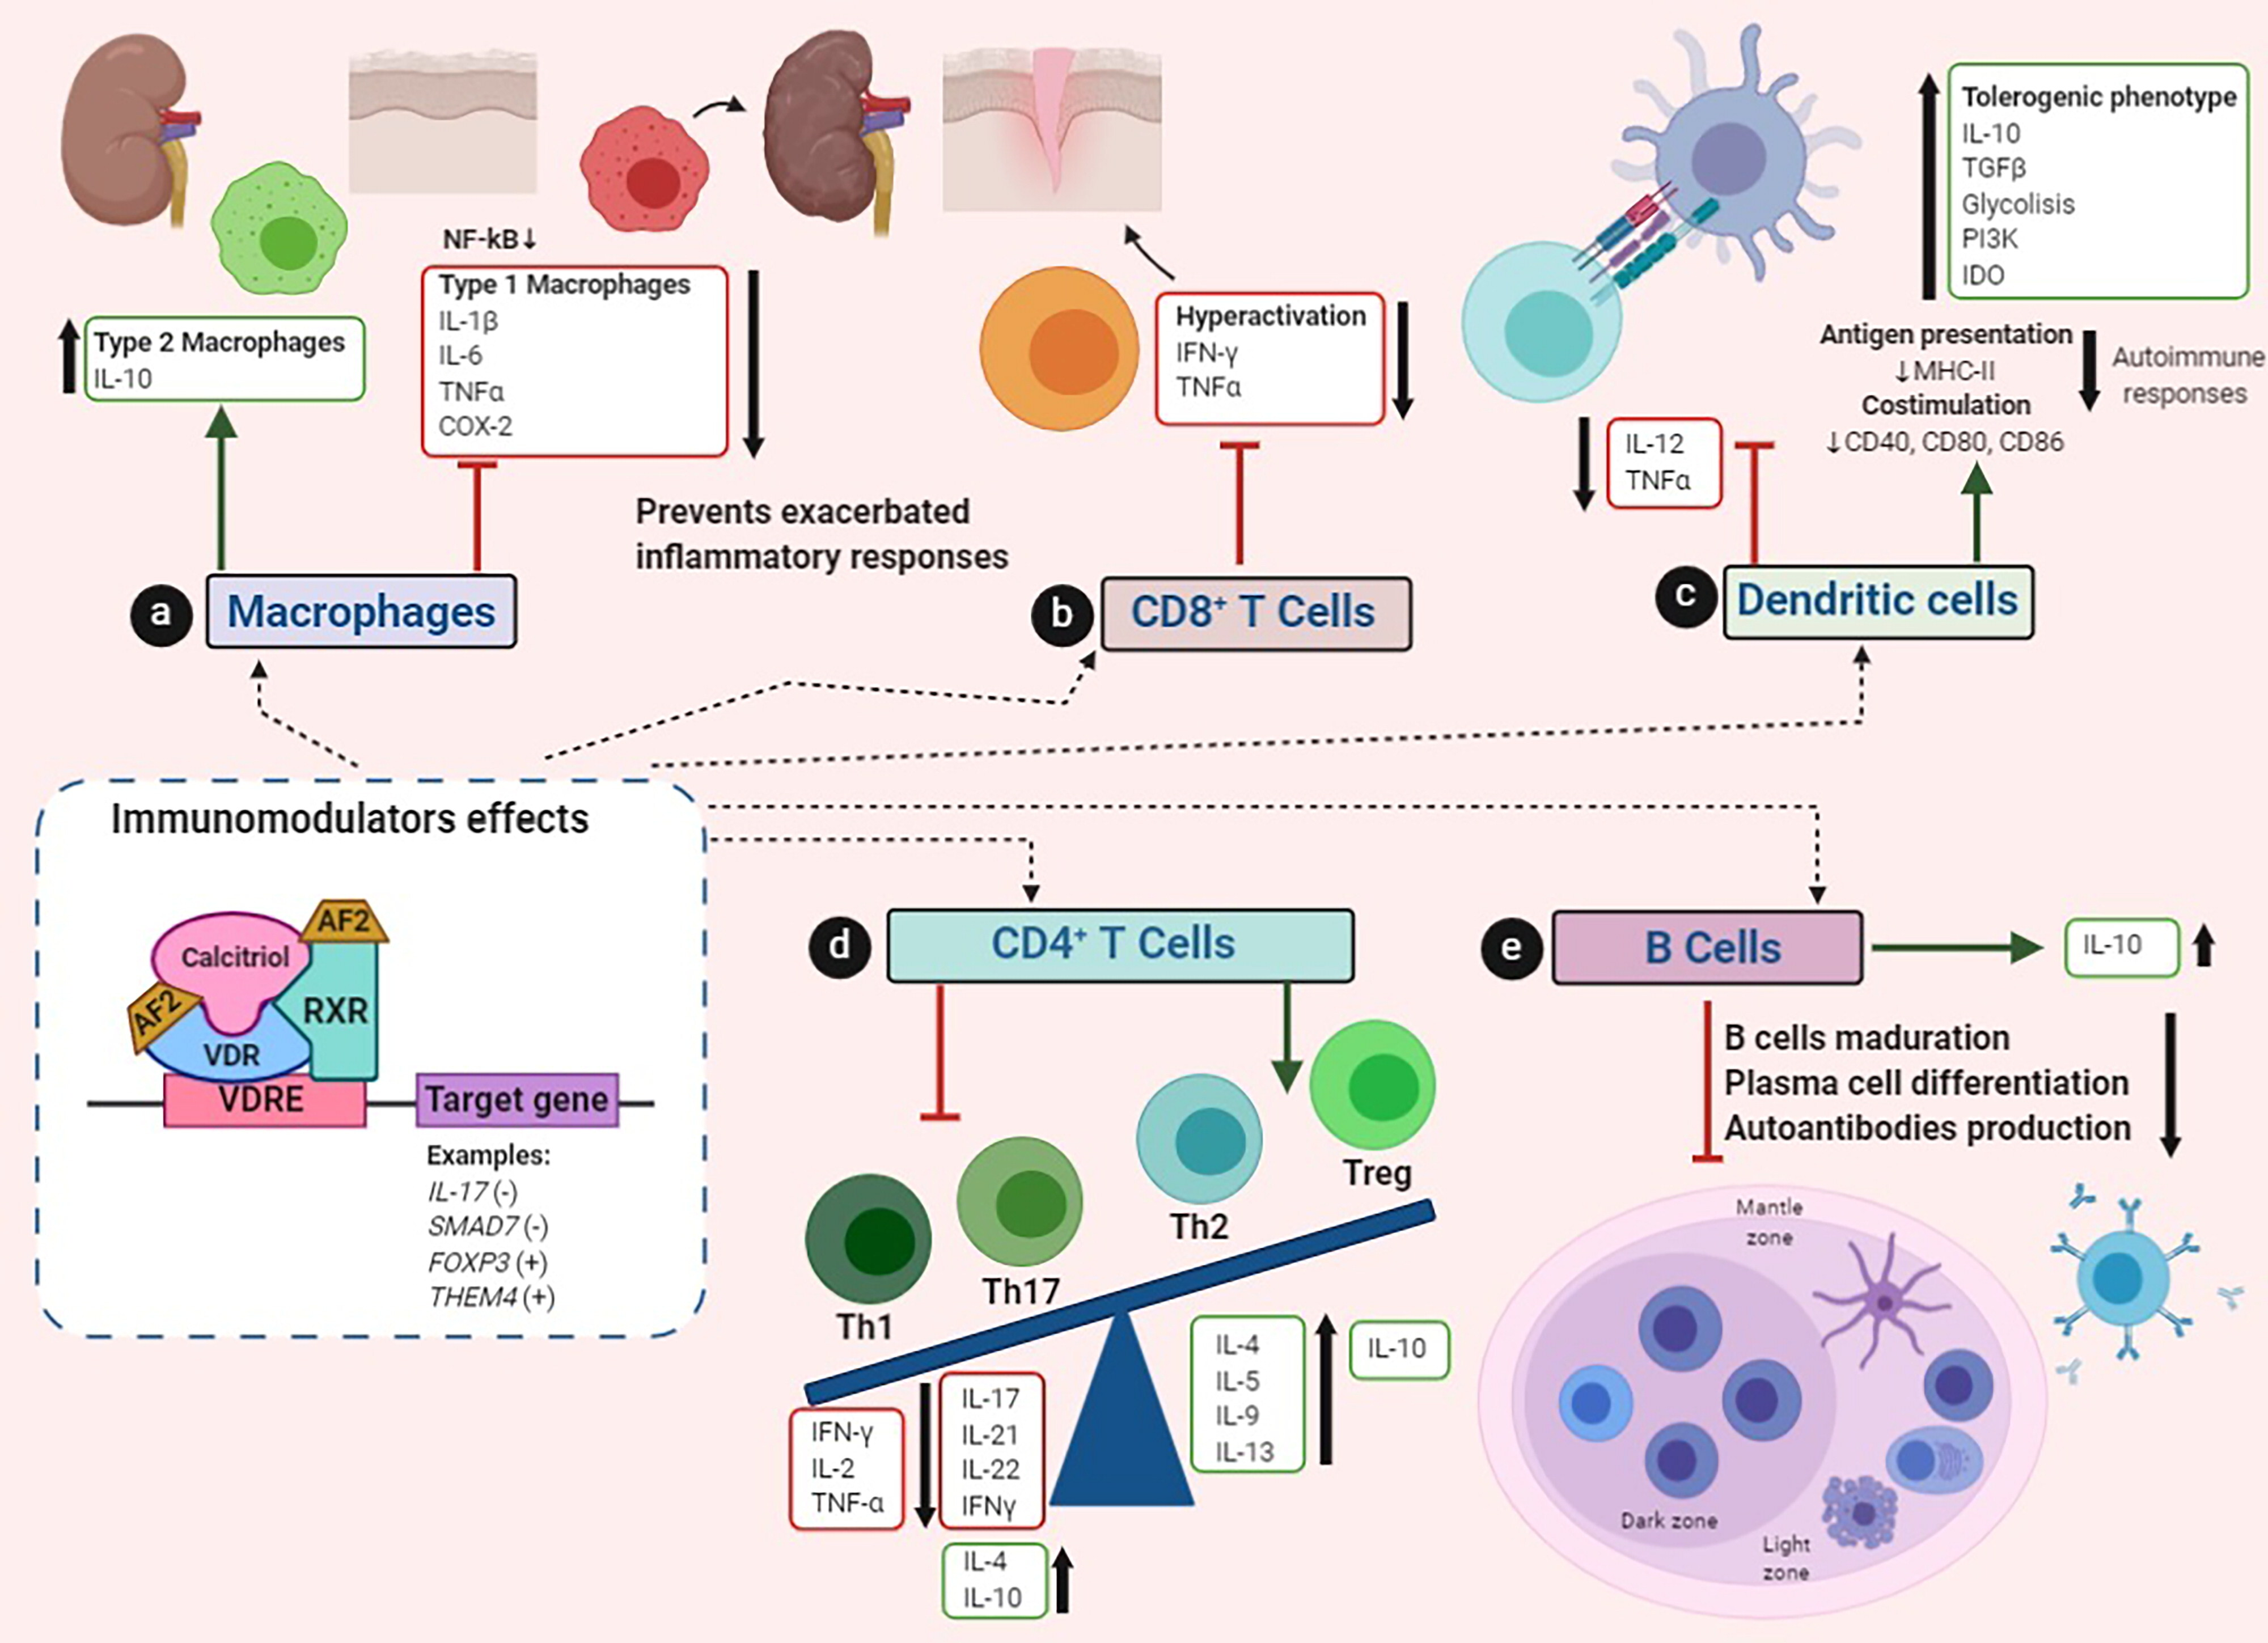
\includegraphics{figures/calcitriol-immunomodulatory.jpg}

}

\caption[Schéma récapitulatif des effets immunomodulateurs du
calcitriol.]{\label{fig-immunomod}\textbf{Schéma récapitulatif des
effets immunomodulateurs du calcitriol.} Le calcitriol se fixe sur le
\ac{VDR} qui en interagissant avec le \ac{VDRE} provoque une
transcription de gènes régulateurs de l'immunité, conduisant à des
effets globalement favorisant la suppression et tolérance immunitaire.
Cette modulation se manifeste directement par l'inhibition de facteurs
cytokines pro-inflammatoires et l'augmentation de cytokines
anti-inflammatoires ou indirectement en favorisant le phénotype de
cellules immunes immunosuppressives comme les macrophages de type M2,
les sous-types de lymphocytes \ac{Th2} et \ac{Treg} ou le phénotype
tolérogénique des cellules dendritiques \autocite{Meza-Meza.2022}.}

\end{figure}%

\section{Schéma d'une réponse antivirale
classique}\label{schuxe9ma-dune-ruxe9ponse-antivirale-classique}

Les mécanismes de l'immunité innée antivirale sont similaires à ceux
contre les infections bactériennes. Les virus possèdent des motifs
moléculaires associés aux pathogènes viraux (\acsu{PAMP}) reconnu par
les \ac{PRR} \autocite{Iwasaki.2012}. Certains \ac{PRR} endosomaux ou
intracellulaires reconnaissent l'ARN simple et double brin
\autocite{Bishop.2021,Ismailova.2022}.

Cette reconnaissance déclenche des cascades de signalisation qui
induisent la production d'interférons (\acsu{IFN}) de type I, de
cytokines et d'effecteurs antiviraux, constituant des signaux de dangers
du soi afin d'avertir les cellules voisines et le système immunitaire.
Les réponses transcriptionnelles initiales impliquent un nombre limité
de facteurs de transcription clés, notamment les facteurs de régulation
des interférons (IRF3, IRF7), les membres de la famille AP-1 et
\ac{nfkb} \autocite{Bishop.2021,Ismailova.2022}. Les interférons de type
I produites par les cellules infectés et les cellules dendritiques sont
en particulier au coeur de la réponse antivirale, stimulant la réponse
humorale et cellulaire, agissant sur les lymphocytes
CD8\textsuperscript{+} et cellules \ac{NK}, et sont impliqués dans la
différenciation et maturation des cellules dendritiques. De plus, le
complément est activé, participant à la lyse des cellules infectées et à
l'opsonisation des virus \autocite{msd.complement.2024}.

Les cellules effectrices de la réponse antivirale concernent
majoritairement :

\begin{itemize}
\tightlist
\item
  les cellules \ac{NK} qui contribuent à l'apoptose des cellules
  infectées et la sécrétion de cytokines tel que l'\ac{ifng}
  \autocite{Narni-Mancinelli.2013} ;
\item
  les lymphocytes CD8\textsuperscript{+}, qui luttent contre les
  cellules infectées par leur pouvoir cytotoxique après reconnaissance
  de l'antigène viral par la reconnaissance du peptide viral situé sur
  le CMH-I des cellules infectées \autocite{Sigal.2016} ;
\item
  les lymphocytes Th1 pour activer les lymphocytes T
  CD8\textsuperscript{+} spécifiques et contribuent à la production
  d'IL-2, \ac{ifng}, et de \ac{tnfa} ;
\item
  les cellules dendritiques qui jouent un rôle de présentateur
  d'antigènes et d'activation des lymphocytes T naïfs, et polarisent la
  réponse CD4\textsuperscript{+}, et recrutent les cellules effectrices
  de la réponse immunitaire \autocite{Iwasaki.2012}.
\end{itemize}

\section{Vitamine D et pouvoir
antiviral}\label{vitamine-d-et-pouvoir-antiviral}

Les études montrent globalement que la vitamine D augmente l'immunité
antivirale et en particulier par le biais de la réponse innée immune, et
inhibe les réponses cytokiniques pro-inflammatoires. La vitamine D
possède une implication dans la réponse immunitaire antivirale car de
nombreux virus respiratoires ciblent les cellules épithéliales
pulmonaires, qui sont très sensibles à la présence de vitamine D. Les
cellules épithéliales induisent fortement le \ac{CYP27B1} lors de
présence du calcidiol ainsi que lors de la détection d'ARN viraux double
brins \autocite{Bishop.2021}.

L'induction puissante de la cathélicidine par la vitamine D et la forme
active LL-37, participe à la réponse antivirale en facilitant la
signalisation du TLR3, un détecteur d'ARN à double brin en se liant
directement à cet ARN, transporté dans l'endosome où se situe le TLR3
(\Cref{fig-vd-antiviral}). LL-37 peut avoir une activité virale directe
contre plusieurs virus tel que le virus de la grippe A, le virus
respiratoire syncytial (\acsu{RSV}) en perturbant les membranes virales,
diminuant ainsi la réplication virale
\autocite{Bishop.2021,Ismailova.2022}. En outre, LL-37 participe à la
régénération des tissus \autocite{Ismailova.2022}.

Le peptide antimicrobien défensine \mupbeta 2, induit par la vitamine D,
possède aussi un rôle antiviral où ce rôle a été observé en contribuant
au blocage de l'entrée virale par la perturbation de l'enveloppe virale
\autocite{Bishop.2021}.

Un autre mécanisme a été rapporté concernant l'inhibition de molécules
induites par le rhinovirus. En effet, l'action du calcitriol sur des
cellules du poumons a permis de résister à son infection, en diminuant
l'expression induite par le virus de \ac{ICAM-1}, une molécule de
surface récepteur des rhinovirus et \ac{PAFR} \autocite{Ismailova.2022}

Le calcitriol inhibe le \ac{nfkb} et donc la réponse pro-inflammatoire,
cependant le traitement de cellules infectées par le \ac{RSV} par le
calcitriol ne conduit pas à une augmentation de la charge virale tout en
maintenant l'état antiviral de la cellule
\autocite{Bishop.2021,Zdrenghea.2017}. Il a été observé que lors de
l'infection par le virus de la grippe A chez la souris, le calcitriol
diminue la production d'IL-5 et d'\ac{ifng}.

Il est intéressant de noter que cette induction de cathélicidine dépend
de la concentration en calcidiol, et une concentration insuffisante ne
permet pas une induction de cathélicidine, ce qui renforce l'importance
d'une concentration adéquate en vitamine D appropriée pour le système
immunitaire \autocite{White.2022}.

Comme discuté précédemment, le calcitriol est capable d'induire NOD2 qui
induit l'autophagie pour augmenter la clairance virale. L'autophagie est
un mécanisme clé dans le contrôle de la réplication et l'infection
virale ; la cathélicidine elle-même renforce le mécanisme d'autophagie
en stimulant le facteur Beclin-1 dans les macrophages et monocytes
\autocite{Bishop.2021}.

Il a été rapporté que l'ajout de vitamine D à la thérapie IFNα standard
a permis d'obtenir une efficacité supérieure à celle de l'IFNα seul dans
un modèle de souris transgénique du virus de l'hépatite B
\autocite{Lee.2020}, cependant d'autres études rapportent des résultats
contradictoires.

Globalement la signalisation médiée par la vitamine D renforce le
système immunitaire inné et diminue l'inflammation, cependant les études
ne rapportent pas systématiquement un consensus en raison de la haute
variabilité des résultats et des méthodologies employées
\autocite{Lee.2020}.

\begin{figure}

\centering{

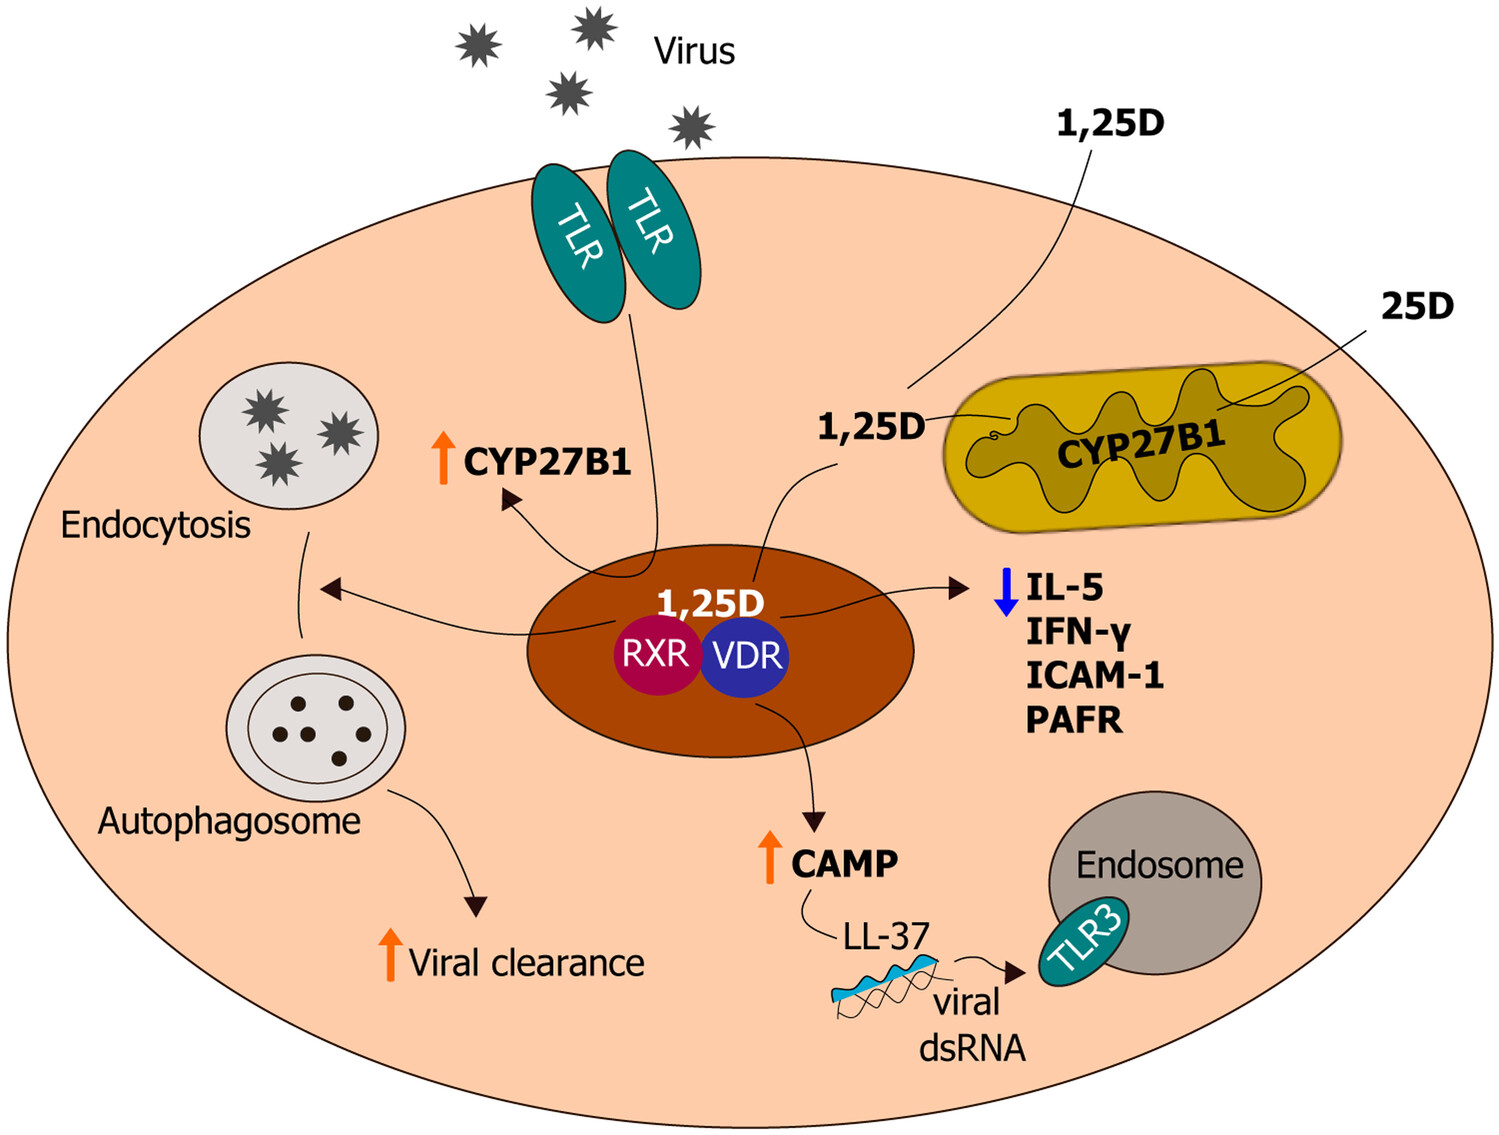
\includegraphics{figures/Ismailova.2022-Antiviral_activity_of_vitamin_D_lung_cell.jpg}

}

\caption[Activité antivirale de la vitamine D dans une cellule
épithéliale pulmonaire.]{\label{fig-vd-antiviral}\textbf{Activité
antivirale de la vitamine D dans une cellule épithéliale pulmonaire.} Le
calcitriol induit plusieurs signaux qui renforce les défenses
antivirales, notamment par l'induction de l'expression de CAMP qui
encode la cathélicidine, dont la forme active LL-37 se lie à l'ADN viral
double brin. Cela permet la reconnaissance par le récepteur endosomal
TLR3, amplifiant la signalisation et l'élimination du virus. De plus, le
calcitriol inhibe les cytokines inflammatoires IL-5 et IFN-γ, et les
molécules ICAM-1 et PAFR. Un autre mécanisme d'élimination virale est
l'induction de l'autophagie. \autocite{Ismailova.2022}.}

\end{figure}%

\section{Metabolisme de la vitamine D dans le système immunitaire
inné}\label{metabolisme-de-la-vitamine-d-dans-le-systuxe8me-immunitaire-innuxe9}

Les cellules immunitaires contrôlent leur propre expression du \ac{VDR}
et du \ac{CYP27B1} afin de moduler les effets du calcitriol sur leur
activation, en fonction des signaux et du statut inflammatoire de
l'environnement. En effet, la \ac{CYP27B1} et le \ac{VDR} peuvent être
induites par les monocytes et macrophages en réponse au signalement des
\ac{PRR} tel que l'activation de CD14-TLR4 (CD14 étant le corécepteur de
TLR4 et une cible d'induction du calcitriol) \autocite{Stoffels.2009},
la stimulation de TLR1 et TLR2 \autocite{Liu.2006}.

Certaines cytokines sont également capables de réguler l'expression de
\ac{CYP27B1} tel que l'\ac{ifng} \autocite{Stoffels.2009} et l'IL-15 en
tant qu'intermédiaire après stimulation du TLR1/2
\autocite{Krutzik.2008}.

Il a été observé que les lymphocytes n'expriment que faiblement le
\ac{VDR} à l'état basal, contrairement aux monocytes, mais fortement
après activation. Les lymphocytes activés expriment également le
\ac{CYP27B1} nécessaire pour convertir le calcidiol en calcitriol
\autocite{Bishop.2021,Charoenngam.2020}.

L'expression de \ac{CYP27B1} et de \ac{VDR} contribue à la synthèse de
calcitriol grâce au calcidiol circulant, et contribue au fonctionnement
du mécanisme immunitaire.

\newpage{}

\chapter{Vitamine D et COVID-19}\label{vitamine-d-et-covid-19}

\section{Physiopathologie de la COVID-19 concernant le système
immunitaire}\label{physiopathologie-de-la-covid-19-concernant-le-systuxe8me-immunitaire}

La \ac{COVID-19} est causée par le virus \ac{SARS-CoV-2} qui est un
virus à ARN simple brin enveloppé qui appartient à la famille des
Coronaviridae. Le virus envahit l'organisme par le biais de la protéine
de pointe appelée spike protein (S). La protéine de pointe est impliquée
dans la liaison aux récepteurs de surface des cellules hôtes, notamment
l'\ac{ACE2}, qui est notamment impliquée dans le \ac{SRAA}
\autocite{Marik.2021}.

La \ac{COVID-19} est caractérisée trois phases cliniques, la phase
d'incubation, la phase symptomatique et la phase pulmonaire
(\Cref{fig-clinical-stage}).

\begin{figure}

\centering{

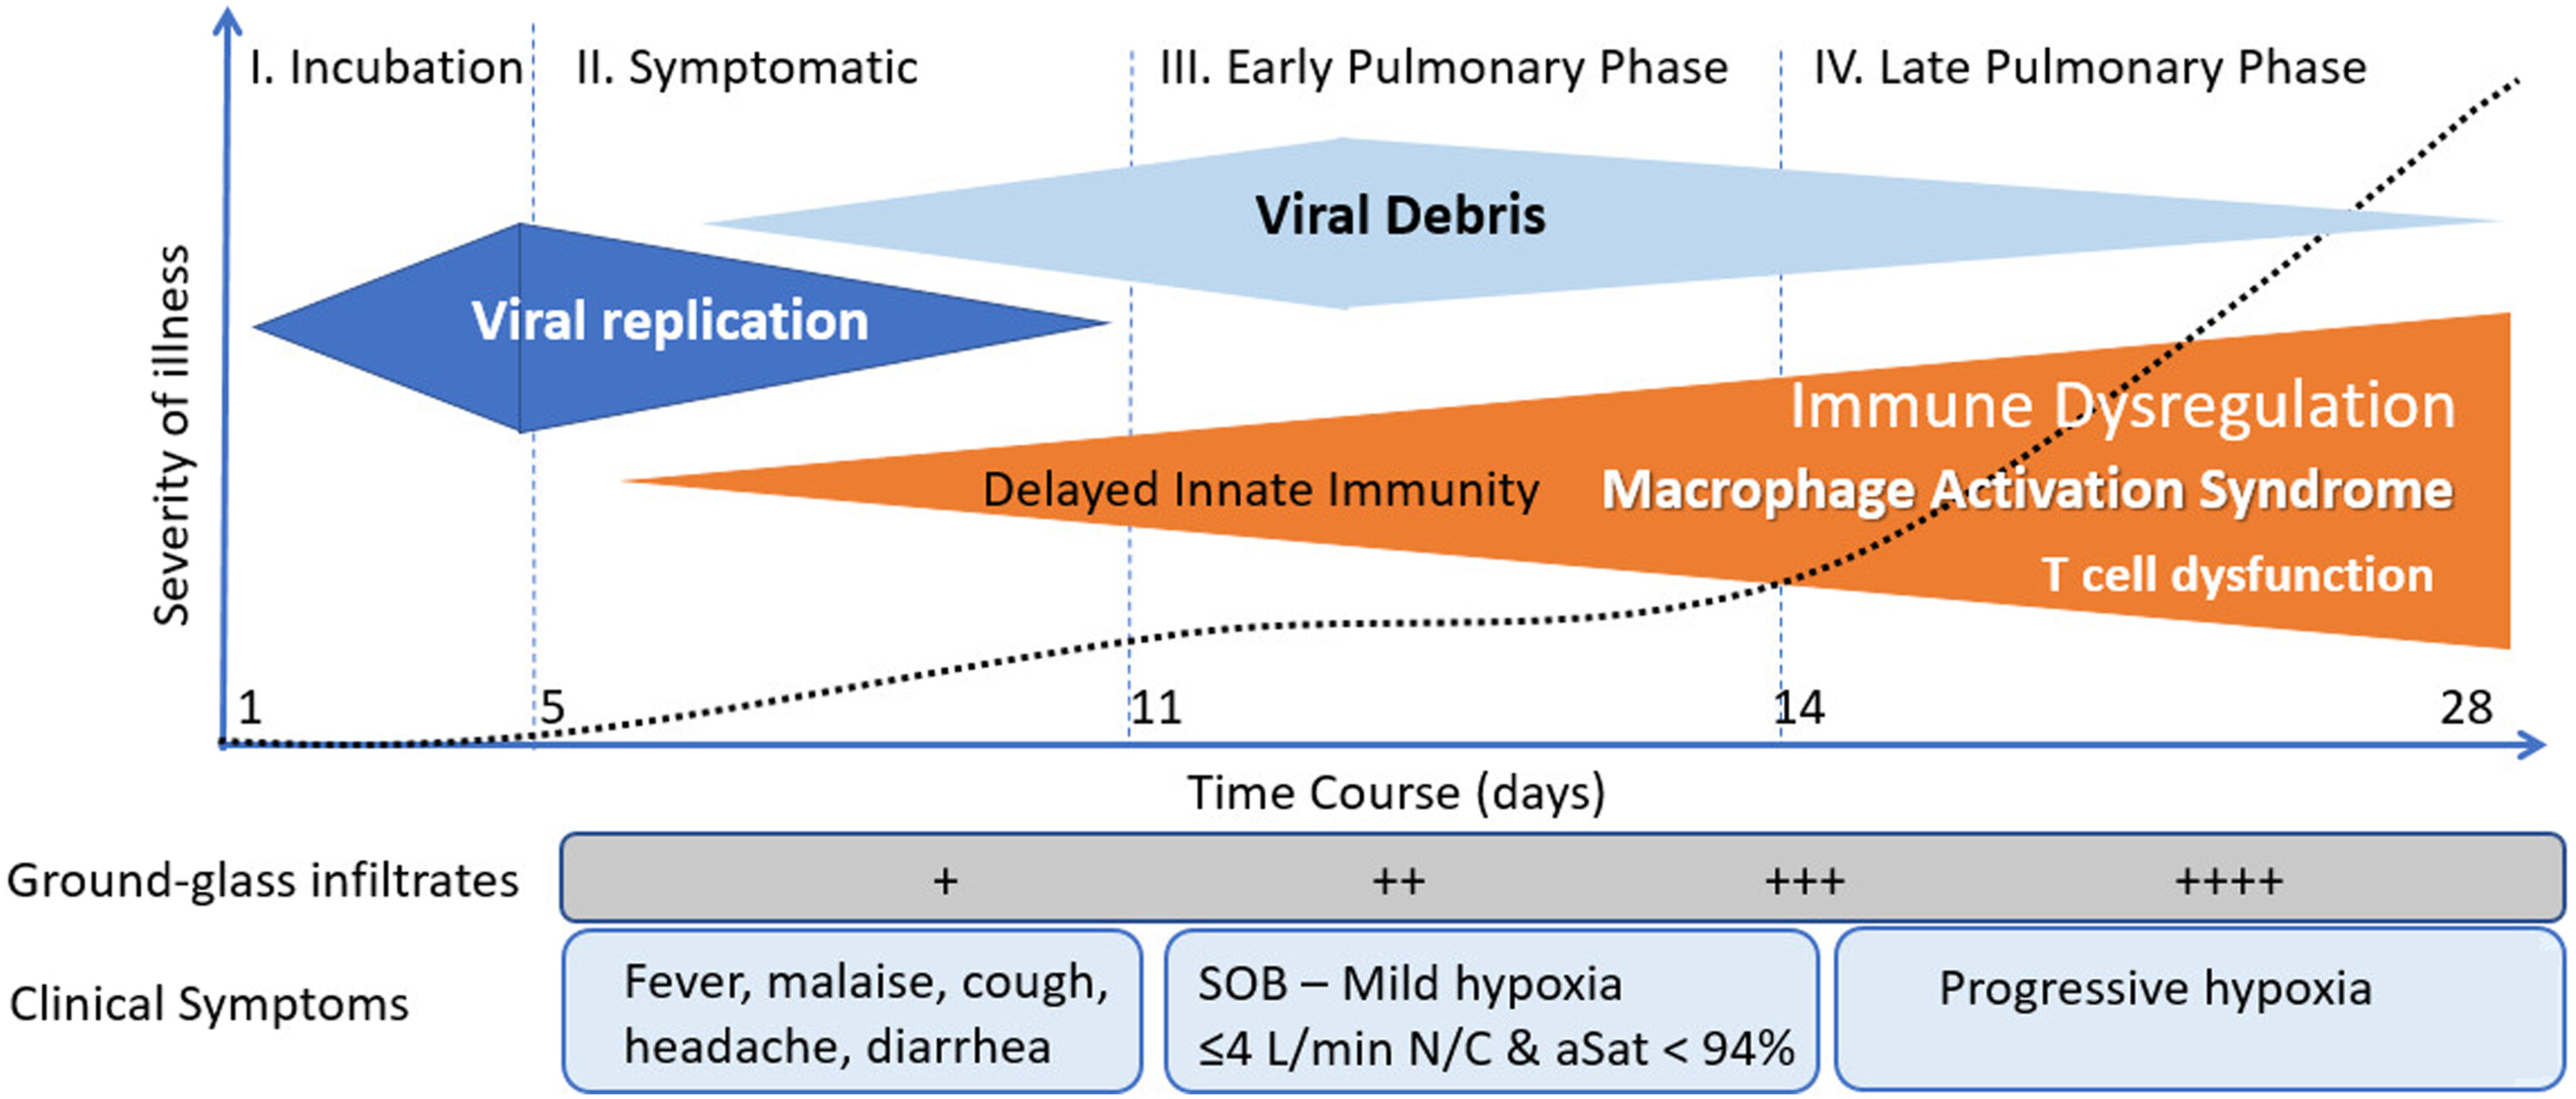
\includegraphics{figures/Marik.2021-Clinical_stages_of_COVID.jpg}

}

\caption[Stages cliniques de la
COVID-19.]{\label{fig-clinical-stage}\textbf{Stages cliniques de la
COVID-19} \autocite{Marik.2021}.}

\end{figure}%

La physiopathologie de la COVID-19 est complexe et implique plusieurs
mécanismes \autocite{Eijk.2021} :

\begin{itemize}
\tightlist
\item
  effets cytopathiques directs du SARS-CoV-2 ;
\item
  diminution de l'\ac{ACE2} avec déséquilibre du \ac{SRAA} et diminution
  de l'inactivation de la bradykinine ;
\item
  réponse immunitaire déréglée caractérisée par une ``tempête de
  cytokines'' ;
\item
  une coagulopathie associée à l'exocytose de facteurs de coagulation,
  une microangiopathie thrombotique ;
\item
  l'auto-immunité.
\end{itemize}

Lorsque la réponse immunitaire n'est plus régulée et devient exacerbée,
si la réplication virale n'est pas contrôlée et les cellules infectées
ne sont pas éliminées, l'état hyperinflammatoire du système immunitaire
peut conduire à un \ac{SDRA} ou une \ac{CIVD}
\autocite{Contreras-Bolívar.2023}.

\subsection{Processus d'infection : entrée dans les cellules hôtes,
réplication
virale}\label{processus-dinfection-entruxe9e-dans-les-cellules-huxf4tes-ruxe9plication-virale}

Durant la phase d'incubation et asymptomatique, le virus infecte les
cellules infecte les cellules épithéliales et les pneumocytes de type
II. Le \ac{SARS-CoV-2} utilise sa protéine de pointe pour se fixer à la
surface des cellules. Une fois attaché à \ac{ACE2}, le virus fusionne
avec la membrane cellulaire, permettant ainsi son entrée dans la cellule
par endocytose avec \ac{ACE2}. Une fois à l'intérieur de la cellule, le
génome viral est libéré, et le virus commence à se répliquer en
utilisant les ressources de la cellule hôte. La réplication virale
aboutit à la production de nombreuses particules virales qui peuvent
infecter d'autres cellules, propageant ainsi l'infection dans le tissu
pulmonaire et au-delà \autocite{Marik.2021,Asselah.2020}.

L'entrée du virus passe plus précisément par deux mécanismes différents
: un mécanisme passant par l'internalisation de ACE2 médié par la
protéine TMPRSS2, clivant la protéine spike S lors de la liaison du
virus à ACE2, et un mécanisme dépendant de la cathepsine L, qui est une
protéase lysosomale, qui clive la protéine spike S après
l'internalisation du virus dans la cellule \autocite{Hoffmann.2020}.

La dysrégulation de \ac{ACE2} impliqué dans le \ac{SRAA} peut causer une
tempête cytokinique et d'autres réponses inflammatoires pathogéniques,
pouvant mener à une défaillance d'organe multiviscérale
\autocite{Argano.2023}.

\subsection{Réponse immunitaire innée et adaptative face à
l'infection}\label{ruxe9ponse-immunitaire-innuxe9e-et-adaptative-face-uxe0-linfection}

Lorsque le SARS-CoV-2 infecte les cellules respiratoires, il déclenche
une série de réponses immunitaires. En temps normal, la cellule infectée
reconnaît la présence du virus grâce aux \ac{PRR} et conduit aux
mécanismes antiviraux discutés précédemment, notamment en activant la
transcription de facteurs de transcriptions pour les interférons, en
particulier les interférons de type I et III, jouant un rôle dans la
défense antivirale restreinte aux cellules épithéliales
\autocite{Maarifi.2020}, et le \ac{nfkb}, conduisant à la production de
cytokines pro-inflammatoires. Cependant le SARS-CoV-2 inhibe la
production d'interférons de type I et III et des gènes stimulés par les
interférons \autocite{Marik.2021}. Un autre moyen de reconnaissance
passe par les cellules dendritiques spécialisées, reconnaissent le virus
par leur \ac{PRR} endosomal, et les macrophages alvéolaires qui
constituent la première ligne de défense.

De manière retardée, le système immunitaire adaptatif est mobilisé
plusieurs jours après l'infection associé à une réponse à interférons
retardée. Les lymphocytes T cytotoxiques CD8\textsuperscript{+}
identifient et détruisent les cellules infectées par le virus, limitant
ainsi la propagation du \ac{SARS-CoV-2}. Les lymphocytes B produisent
des anticorps spécifiques qui peuvent neutraliser le virus. Ensemble,
ces deux composantes de la réponse immunitaire contribuent à contrôler
l'infection \autocite{Marik.2021}.

\subsection{Choc cytokinique}\label{choc-cytokinique}

Lorsque la réponse immunitaire est excessive, conduisant à un \ac{SLS},
elle peut entraîner un choc cytokinique qui est caractérisée par une
libération massive de cytokines pro-inflammatoires, notamment l'IL-1,
l'IL-6 et le \ac{tnfa}, qui contribuent à l'hyperactivation du système
immunitaire dans une boucle de rétroaction positive. Les patients
sévères COVID-19 présentent une lymphopénie et en particulier une
réduction des lymphocytes périphériques, un plus haut niveau de
cytokines (IL-6, IL-10, G-CSF, \ac{ifng}, \ac{MIP-1}, \ac{MCP-1} et
\ac{tnfa}), avec une corrélation entre les niveaux d'IL-6 et la sévérité
de la maladie \autocite{Yuki.2020}.

De plus, des marqueurs d'exhaustion ont été observé sur les lymphocytes
et cellules NK; l'exhaustion des cellules immunes peut conduire à une
progression de la maladie \autocite{Yuki.2020}. Le système immunitaire
est suractivé de manière dysfonctionnelle, en particulier la
suractivation des lymphocytes CD4\textsuperscript{+} et
CD8\textsuperscript{+} et Th17 est observé \autocite{Xu.2020}.
Notamment, l'IL-17 produite par le Th17 est impliqué dans des risques de
thrombose et de \ac{SDRA} \autocite{Raucci.2020}.

Chez le patient COVID-19 sévère, la réponse inflammatoire continue est
due à l'hyperactivation du système immunitaire plutôt qu'à une
défaillance de la clairance virale. Les macrophages activés continuent
de produire des cytokines après l'élimination du virus, et ne sont pas
enlevés, possiblement à cause de l'échec des cellules NK et lymphocytes
CD8\textsuperscript{+} dû à un phénotype d'épuisement
\autocite{Marik.2021}. De plus, les macrophages possèdent le récepteur
ACE2, et l'infection des macrophages conduit à une production de
cytokines pro-inflammatoires ce qui exacerbe l'inflammation
\autocite{Marik.2021}.

La tempête cytokinique endommage les poumons et causer une infiltration
pulmonaire et une sévère hypoxie, résultant en une dysfonction de la
respiration. Elle est également impliquée lors des défaillances
d'organes multiviscérales \autocite{Argano.2023}.

Une complication grave et mortelle des patients COVID-19 allant dans les
services de soins intensifs est le sepsis. Le sepsis est caractérisé par
une réaction immunitaire excessive et incontrôlée à une infection,
pouvant entraîner une défaillance multiviscérale et engager le pronostic
vital.

\section{Rationnel du mécanisme physiologique de l'usage de la vitamine
D dans la
COVID-19}\label{rationnel-du-muxe9canisme-physiologique-de-lusage-de-la-vitamine-d-dans-la-covid-19}

Trois mécanismes principaux supportent l'action de la vitamine D
\autocite{Pal.2022,Borsche.2021} :

\begin{itemize}
\tightlist
\item
  Régulation négative du \ac{SRAA} en promotant l'axe ACE2/Ang(1-7)/MasR
  (\aclu{Ang(1-7)}, \aclu{MasR}) et en diminuant l'axe ACE\}/Ang II/
  AT1R (\aclu{Ang II}, \aclu{AT1R}).
\item
  L'induction de la cathélicidine et de défensines pour leur protection
  antivirale ;
\item
  Régulation de la production de cytokines pro-inflammatoires et
  induction de cytokines anti-inflammatoires en diminuant la production
  de Th1 et en promotant la différence de \ac{Treg}, diminuant le
  \ac{SLS} ;
\end{itemize}

\subsection{Système Rénine Angiotensine
Aldostérone}\label{systuxe8me-ruxe9nine-angiotensine-aldostuxe9rone}

La physiopathologie de la COVID-19 implique le \ac{SRAA} causé en
premier temps par l'entrée du virus dans les cellules, ce qui provoque
l'endocytose du récepteur-enzyme \ac{ACE2} et inhibe ainsi ses fonctions
en diminuant l'expression membranaire de \ac{ACE2}, puisque la forme
effective de \ac{ACE2} est membranaire ou soluble
\autocite{Donoghue.2000}. \ac{ACE2} est une enzyme importante dans le
\ac{SRAA}, qui possède un effet antagoniste du récepteur \ac{ACE}, les
deux agissant comme une balance afin de réguler diverses fonctions
physiologiques telles que la pression artérielle, l'inflammation, la
fibrose, la prolifération cellulaire, la régénération tissulaire, et la
réponse immunitaire (\Cref{fig-sraa-covid19})
\autocite{Brojakowska.2020}. En effet, \ac{ACE2} régule la concentration
de \ac{Ang II} en catalysant sa conversion en \ac{Ang(1-7)} et régule
donc les effets de \ac{Ang II} passant par la liaison au récepteur
\ac{MasR} ; ACE2 diminue l'action médiée par l'\ac{Ang II} survenant par
sa liaison au récepteur AT1 \autocite{Gotelli.2022}. L'infection par le
SARS-CoV-2 régule à la baisse l'activité d'\ac{ACE2} ce qui cause une
accumulation de \ac{Ang II} qui peut causer des conséquences de la
suractivation du SRAA (\Cref{fig-sraa-covid19}) \autocite{Mahdavi.2020}.

De plus, \ac{ACE2} n'est pas seulement le récepteur d'entrée du
SARS-CoV-2 mais pourrait jouer un rôle dans la régulation immune en
agissant par d'autres mécanismes indirects \autocite{Jiang.2014}, tel
que la réduction du stress oxydatif, l'inhibition de la \ac{NOS},
l'inhibition de la \ac{COX-2}, dans divers tissus \autocite{Jiang.2014}.
Un mécanisme notable consiste en l'interaction de \ac{ACE2} avec les
protéines \ac{ADAM17} et \ac{TMPRSS2} qui modulent des cytokines
pro-inflammatoires \autocite{Zipeto.2020}. \ac{TMPRSS2} est une sérine
protéase d'intérêt car elle est impliquée dans la fusion directe du
virus avec la membrane cellulaire, et clive également \ac{ACE2}.
Similairement, \ac{ADAM17} est une métalloprotéase qui clive \ac{ACE2},
et son activité est augmentée lorsque \ac{ACE2} est internalisé.
\ac{ADAM17} peut conduire à la libération de \ac{tnfa} et IL6R, ainsi
que d'autres molécules proinflammatoires. L'axe Ang II-AT1R active
\ac{ADAM17} qui libère à son tour la forme mature de l'EGFR, la forme
soluble de l'IL-6Ra et le \ac{tnfa}. L'\ac{Ang II} n'agit donc pas
seulement comme un vasoconstricteur mais aussi comme une molécule
pro-inflammatoire par l'intermédiaire de la liaison à AT1R.

La dysrégulation de \ac{ACE2} impliqué dans le \ac{SRAA} peut causer une
tempête cytokinique résultante du déséquilibre du système, une pneumonie
et d'autres réponses inflammatoires pathogéniques pouvant mener à une
défaillance d'organe multiviscérale \autocite{Argano.2023}.

\begin{figure}[!htbp]
    \centering
    \begin{subfigure}
        {\textwidth}
        \centering
        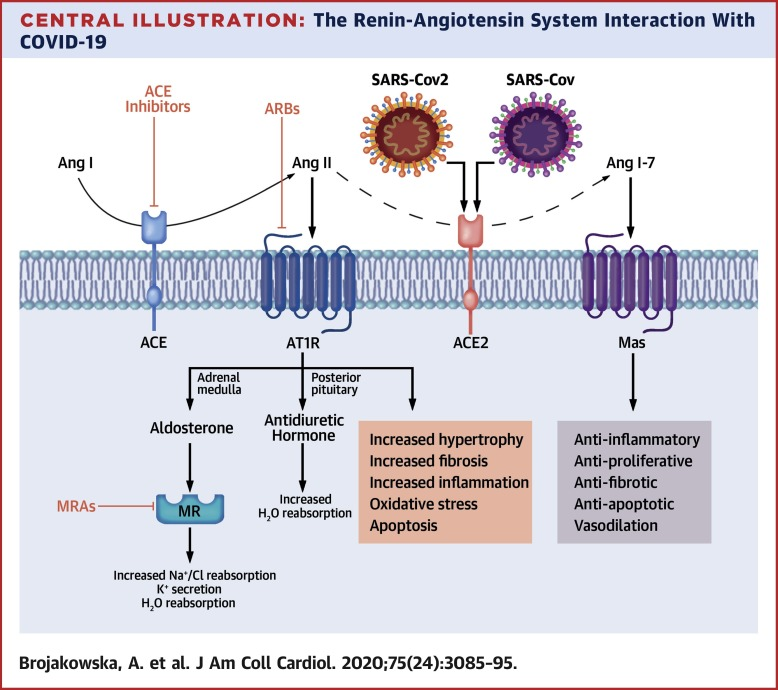
\includegraphics[width=0.8\textwidth]{figures/Brojakowska-RAS-COVID-19.jpg}
        \caption{\textbf{Interaction du SRAA avec la COVID-19} \autocite{Brojakowska.2020}.}
        \label{fig-sraa-covid19}
    \end{subfigure}

    \bigskip

    \begin{subfigure}
        {\textwidth}
        \centering
        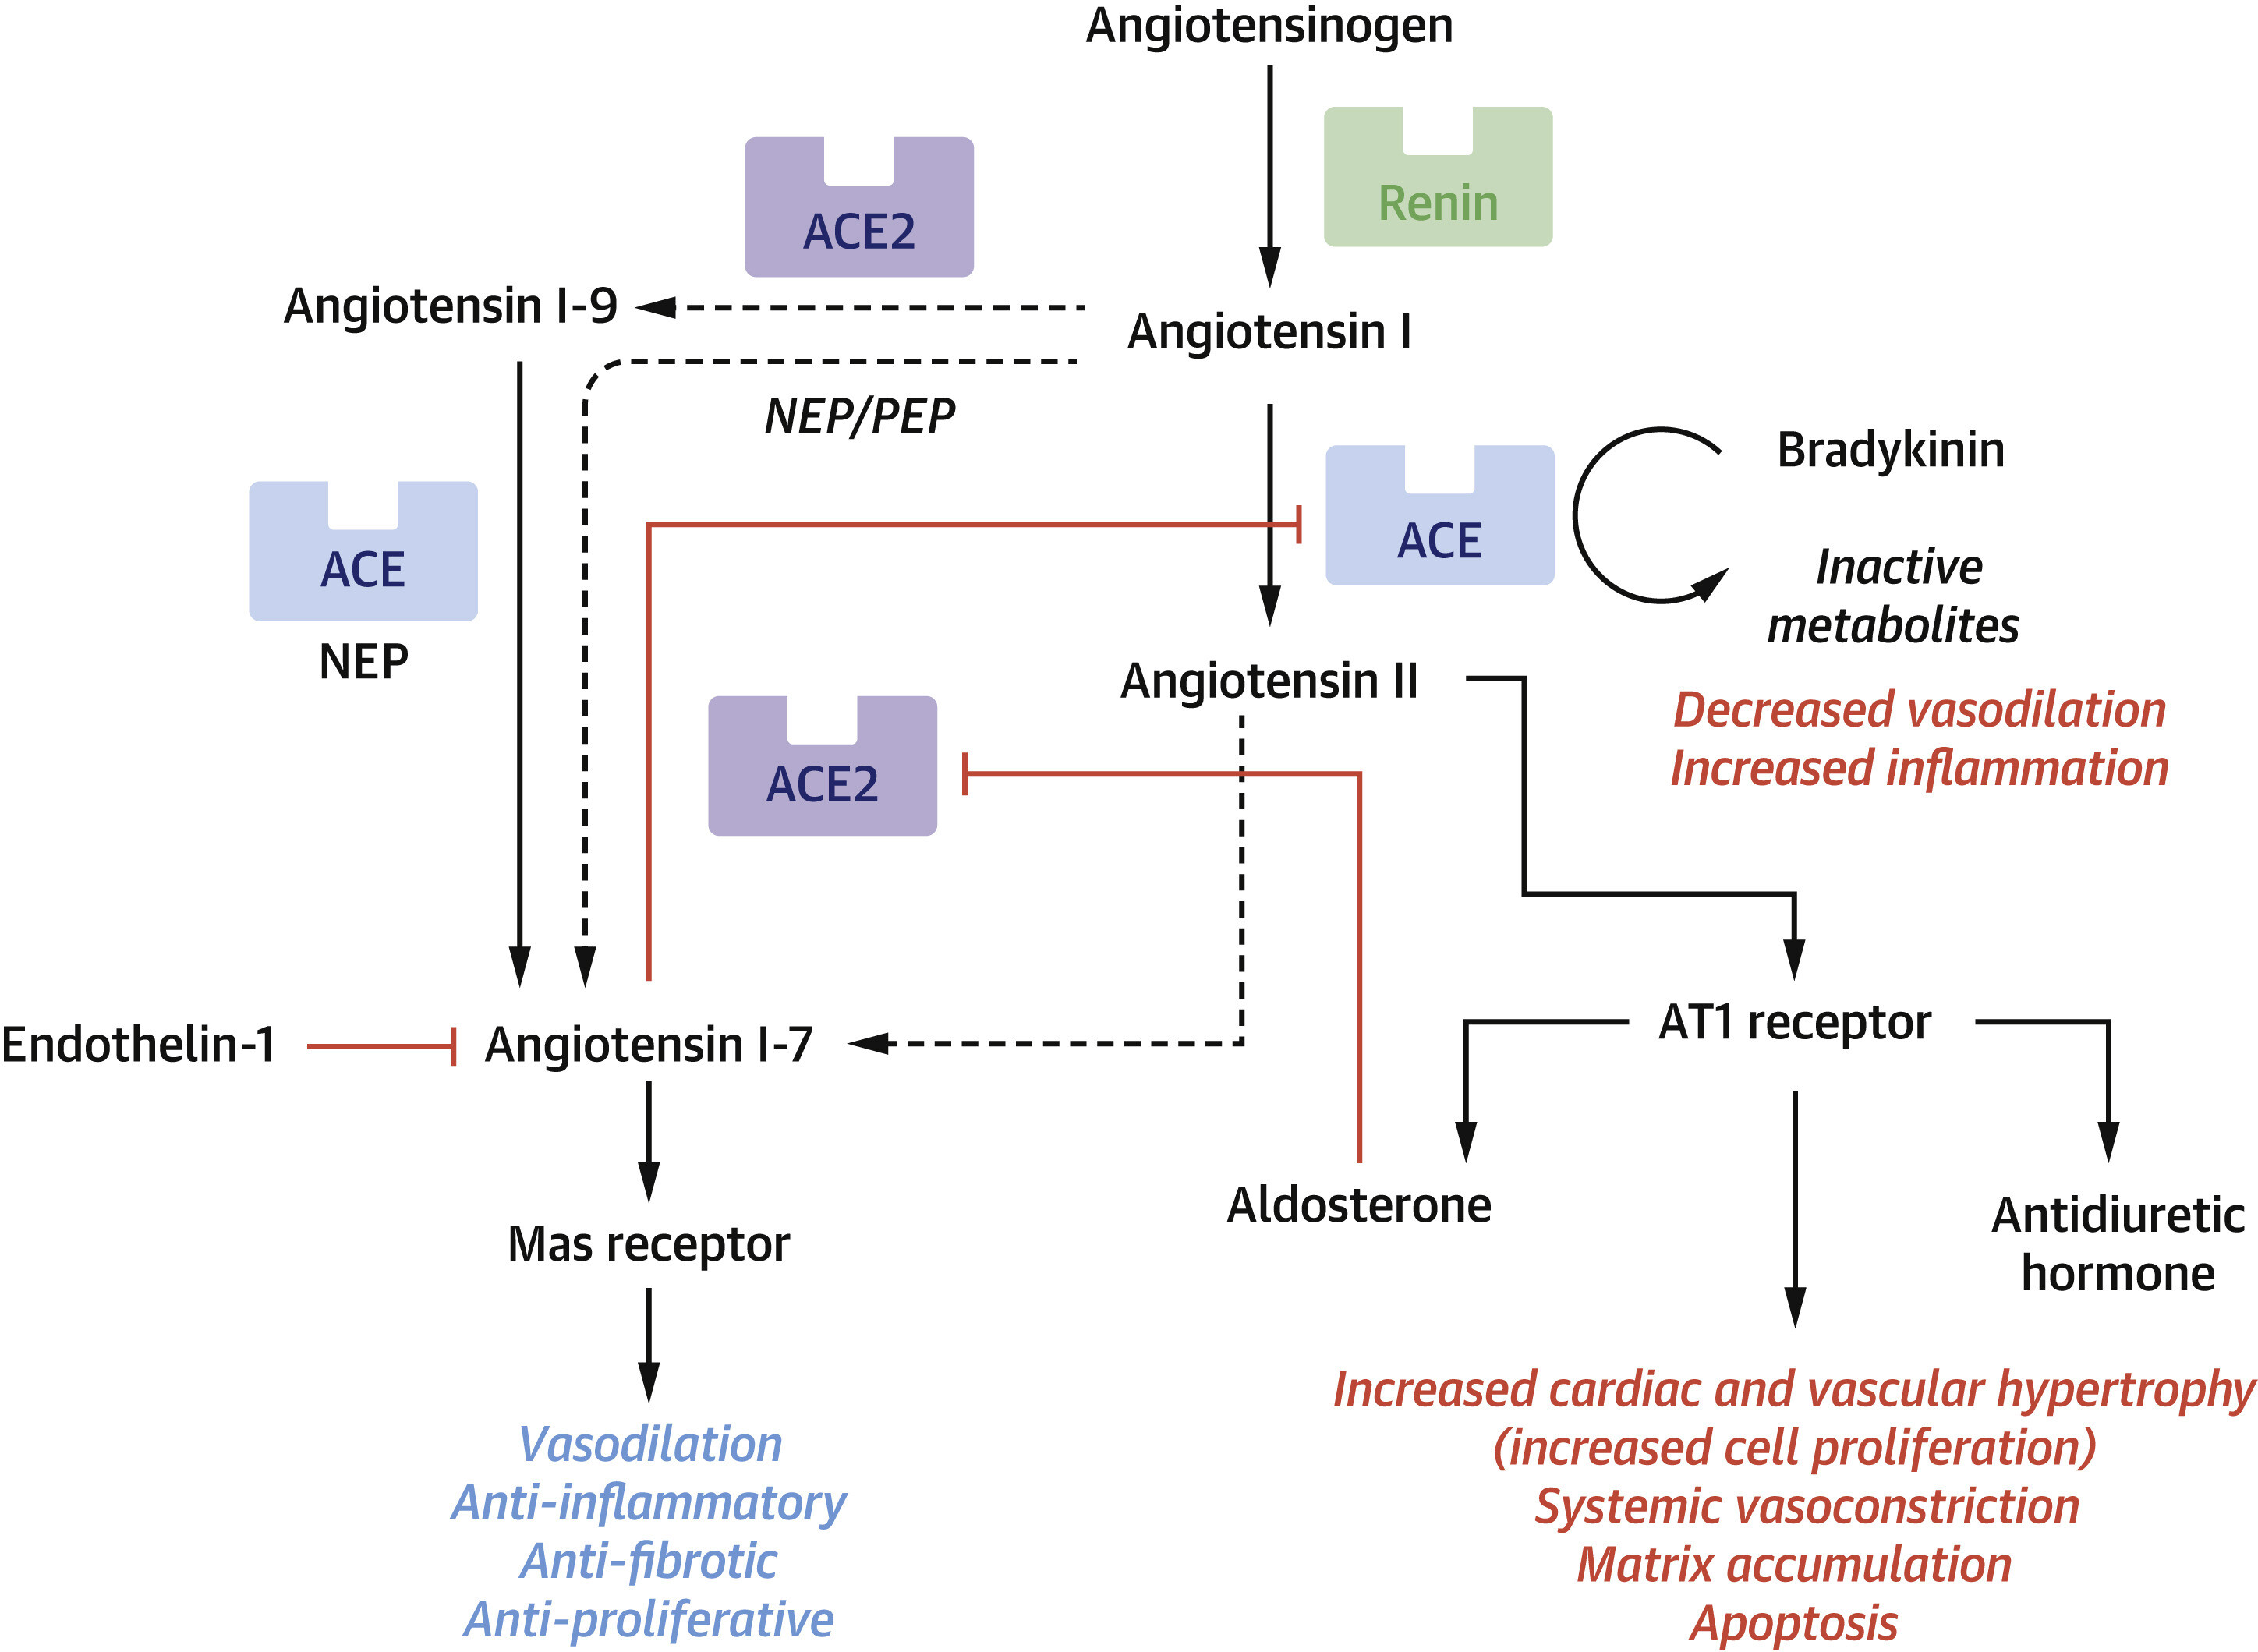
\includegraphics[width=0.8\textwidth]{
            figures/Brojakowska-RAS-ACE2-Regulation.jpg
        }
        \caption{\textbf{Régulation du SRAA et de l'axe ACE2/Ang-1-7/AT1/MasR} \autocite{Brojakowska.2020}.}
        \label{fig-ace2-masR}
    \end{subfigure}
    \caption[Interaction du SRAA avec la COVID-19 et régulation du SRAA et de l'axe
    ACE2/Ang-1-7/AT1/MasR.]{\textbf{Interaction du SRAA avec la COVID-19 et
    régulation du SRAA et de l'axe ACE2/Ang-1-7/AT1/MasR.}}
\end{figure}

La vitamine D agit sur deux principaux évènements mettant le pronostic
vital en jeu dans la physiopathologie de la \ac{COVID-19}, le \ac{SDRA}
et le \ac{SLS}, par un mécanisme particulier spécifique entre la
vitamine D et le \ac{SARS-CoV-2} \autocite{Borsche.2021} concernant le
\ac{SRAA} : la vitamine D agit comme modulateur négatif du \ac{SRAA} en
diminuant l'expression de rénine et en augmentant celle de \ac{ACE2} ;
la diminution de l'\ac{Ang II} et l'augmentation de \ac{Ang(1-7)}
favorisant la voie \ac{MasR} et donc un état anti-inflammatoire. Il a
été observé que lorsque le \ac{VDR} est KO dans une étude chez les
souris, l'activité du \ac{SRAA} est augmentée. L'ajout de vitamine D
diminue la production de rénine \autocite{Li.2002}, ce qui justifie le
caractère régulateur de la vitamine D sur le \ac{SRAA}. De même, le
calcitriol diminue le ratio \ac{ACE}/\ac{ACE2}, diminuant l'induction de
\ac{ACE} et la suppression de \ac{ACE2} chez les rats diabétiques,
réprime le récepteur AT1 de l'\ac{Ang II} et \ac{ACE}, et réduit la
formation de \ac{Ang II}, tout en augmentant l'expression des éléments
\ac{ACE2}, \ac{Ang(1-7)}, \ac{MasR} \autocite{Mahdavi.2020}.

En outre, il a été montré que l'\ac{Ang II} diminue l'expression du
\ac{CYP27B1} et donc exacerbe la déficience en vitamine D
\autocite{Borst.2011}.

Un autre mécanisme passant par la bradykinine est impliqué dans les
processus perturbés par la \ac{COVID-19}. \ac{ACE} est responsable de la
dégradation de la bradykinine, régulant la pression artérielle,
induisant la vasodilatation, perméabilité vasculaire, natriurèse et
hypotension (\Cref{fig-ace2-masR}). La bradykinine serait également
impliqué lors de l'inflammation car elle induit le recrutement des
neutrophiles et une augmentation de la perméabilité vasculaire.
L'analyse computationnelle de l'expression des gènes des fluides de
lavages bronchoalvéolaires de \textcite{Garvin.2020} révèle une
``tempête bradykinique'', où l'expression de bradykinine chez les
patients \ac{COVID-19} est en surreprésentation par rapport aux patients
contrôles. De plus, l'expression de \ac{ACE2} est également
surreprésentée chez les patients \ac{COVID-19}, ce qui implique une
régulation négative de \ac{ACE} par \ac{ACE2}, conduisant à une
augmentation de la bradykinine. La tempête bradykinique explique la
plupart de la symptomatologie de la \ac{COVID-19}
\autocite{Garvin.2020}. Les auteurs notent une diminution de
l'expression de vitamine D et de VDR, ce qui diminue l'expression de
rénine et altère la régulation de ACE2. Cette étude, à l'inverse des
autres, montre que l'axe \ac{ACE2} est surreprésenté et que la
bradykinine est augmentée, ce qui est en contradiction avec les autres
études qui montrent une diminution de ACE2 et une augmentation de Ang II
Les auteurs suggèrent que la vitamine D pourrait être un traitement
potentiel pour la \ac{COVID-19} en régulant l'axe ACE2/bradykinine par
l'inhibition de rénine.

\begin{figure}

\centering{

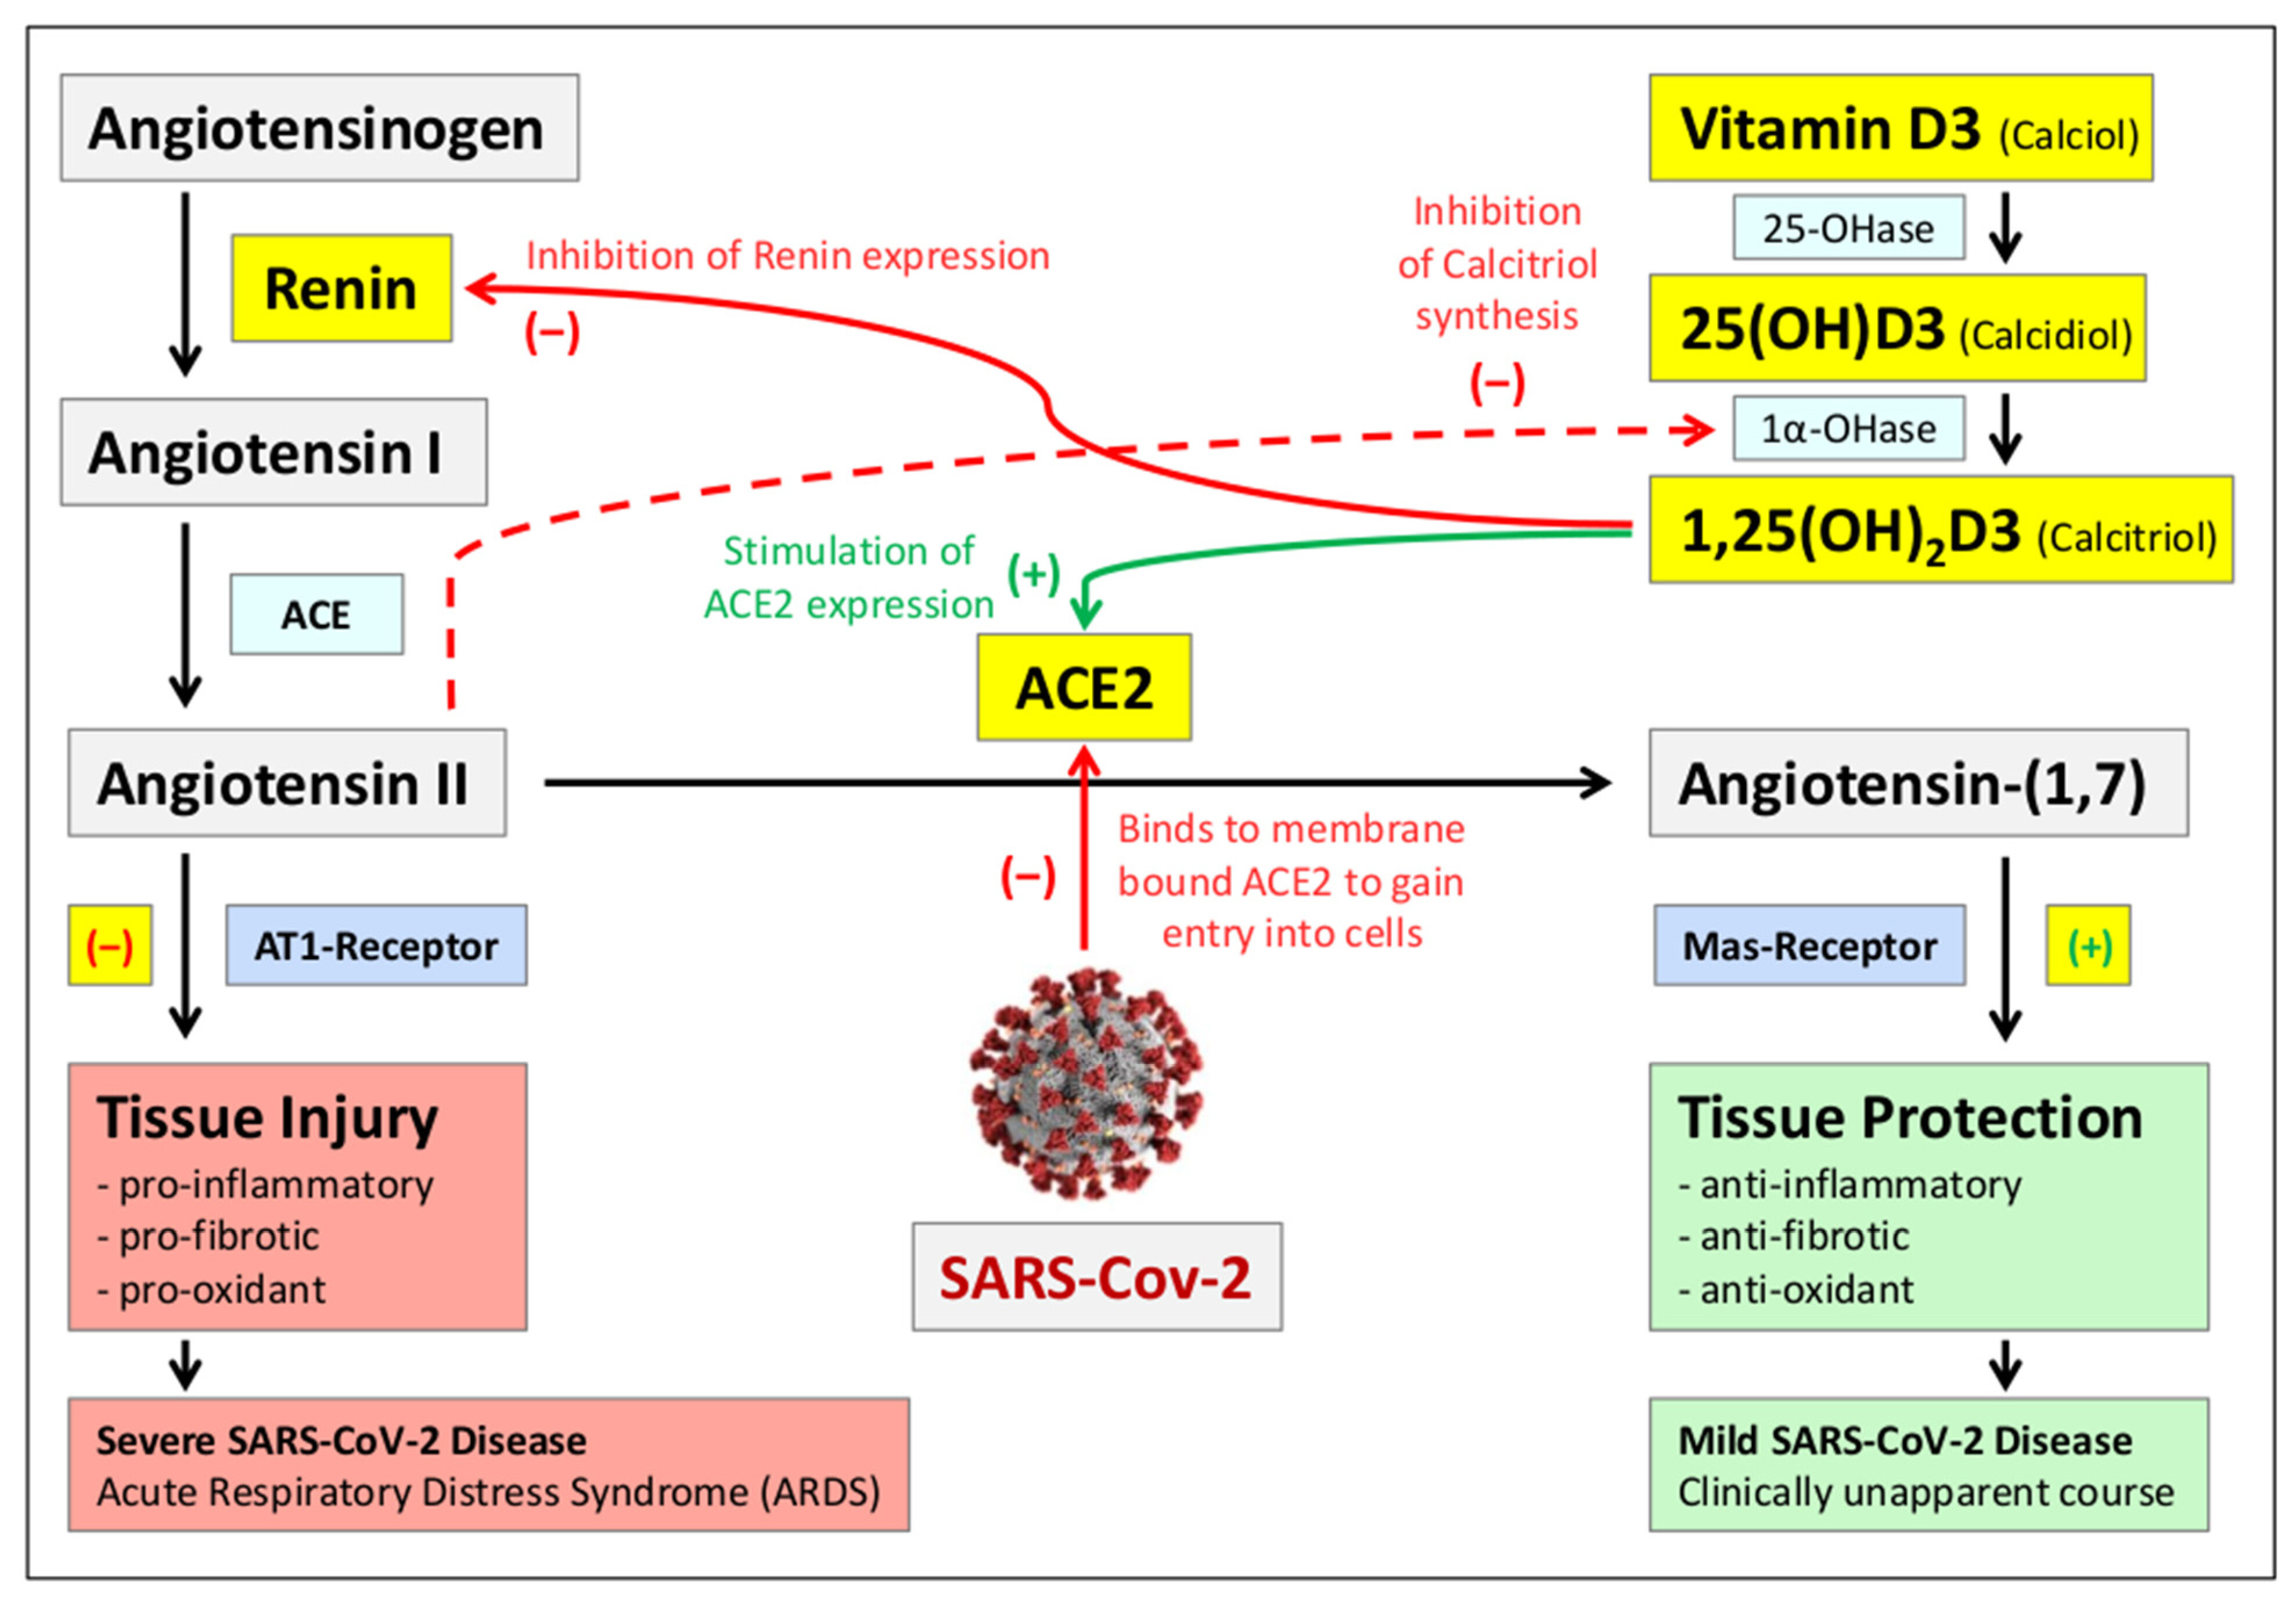
\includegraphics{figures/borsche.2021-vd-ras.jpg}

}

\caption[Schéma du rôle du la vitamine D dans l'inhibition du
SRAA.]{\label{fig-vd-ras}\textbf{Schéma du rôle du la vitamine D dans
l'inhibition du SRAA \autocite{Borsche.2021}.}}

\end{figure}%

\subsection{Mécanisme lié l'inhibition de
l'hyperinflammation}\label{muxe9canisme-liuxe9-linhibition-de-lhyperinflammation}

Généralement, les actions de la vitamine D sur la réponse immunitaire au
SARS-CoV-2 sont similaires aux effets observés de la vitamine D sur le
système immunitaire, décrit dans la partie sur l'action immunomodulateur
de la vitamine D (\textbf{Section~\ref{sec-immunomodulateur}}). La
vitamine D diminue l'hyperinflammation pathologique fréquemment associée
lors du COVID-19.

\subsubsection{Mécanisme impliquant l'immunité
innée}\label{muxe9canisme-impliquant-limmunituxe9-innuxe9e}

\begin{figure}

\centering{

\includegraphics{figures/Contreras-Bolívar.2023-vd_paracrine_intracrine_functions.jpg}

}

\caption[Représentation schématique des fonctions paracrines et
intracrines de la vitamine D et de ses métabolites et actions dans les
systèmes immunitaires innés et
adaptatifs.]{\label{fig-vd-covid-function}\textbf{Représentation
schématique des fonctions paracrines et intracrines de la vitamine D et
de ses métabolites et actions dans les systèmes immunitaires innés et
adaptatifs.} A : Synthèse de la vitamine D. B1 : Immunité adaptative. B2
: immunité innée. C : Réponse inflammatoire médiée par le SARS-CoV-2
\autocite{Contreras-Bolívar.2023}.}

\end{figure}%

Le calcitriol contribue à la réponse antimicrobienne par l'induction de
cathélicidine, défensine, et favorise la chimiotaxie des neutrophiles et
macrophages sur le lieu de l'infection. En effet, il a été observé
\emph{in vitro} que le LL-37 se lie avec une grande affinité à la
protéine de pointe S du SARS-CoV-2, empêchant celle-ci de se lier à la
cellule hôte. LL-37 masque simultanément les sites de liaisons de
\ac{ACE2} au domaine de liaison du récepteur du virus
\autocite{Wang.2021.ACS}. Le calcitriol favorise l'autophagie par le
biais de LL-37, qui est un mécanisme de défense contre les infections
virales et peut inhiber la réplication virale \autocite{Gotelli.2022}.
En effet, la présence de LL-37 est nécessaire pour l'induction de
l'autophagie dans les macrophages et les monocytes et de la formation
des autophagosomes, qui est fortement diminuée lorsque LL-37 est KO. Ce
mécanisme d'induction passe par l'activation de \ac{MAPK} médié par
l'induction de Beclin-1 et Atg \autocite{Yuk.2009}. De plus, un autre
mécanisme possible de l'activation de l'autophagie passe par le
signalement du calcium au niveau de la mitochondrie et du réticulum
endoplasmique, par la voie \ac{CaMKKβ} et \ac{AMPK}, activant la voie
mTOR \autocite{Yuk.2009,Shiravi.2022}. Puisque le SARS-CoV-2 inhibe
l'autophagie par l'inhibition de promoteur de l'autophagie comme la
cible \ac{mTORC1}, la voie \ac{AMPK}, et la dégradation Beclin-1
\autocite{Gotelli.2022}, qui sont aussi des cibles de la vitamine D, il
est possible que la vitamine D puisse avoir un impact positif en
restaurant ces mécanismes.

L'action du calcitriol sur l'immunité innée conduit à une augmentation
de la neutralisation et clairance du virus, ainsi que la réduction de la
production de cytokines et de l'action pro-inflammatoire des
neutrophiles, macrophages et cellules dendritiques
(\Cref{fig-vd-covid-function}). Ainsi, le calcitriol promeut ainsi le
phénotype M2 des macrophages par la synthèse de l'IL-10. Le calcitriol
peut en outre atténuer le TLR2 qui reconnaît le SARS-CoV-2 et engendre
une cascade inflammatoire, inhiber la voie subséquente de \ac{nfkb} et
l'inflammasome NLRP3 dans des modèles animaux et humains inflammatoires
\autocite{Gotelli.2022}. Les cellules dendritiques possèdent une réponse
à l'interféron I réduite ainsi que la sécrétion de IL-12 et IL-23 lors
de l'infection à la COVID-19. De ce fait, la vitamine D favorise un rôle
tolérogénique superposable à l'état de la cellule dendritique.
Concernant les neutrophiles, la NETose est En effet la vitamine D
stimule la production de LL-37 par les neutrophiles, qui par le biais
des macrophages, induit le retrait de NETose qui a été observé comme
favorisant l'infection par le SARS-CoV-2 au lieu de conférer un rôle
protecteur \autocite{Gotelli.2022}.

De manière indirecte, il existe une action potentielle de la vitamine D
par le biais du transporteur \ac{DBP}, qui recrute les neutrophiles et
active le complément C5a, induisant une inflammation systémique ; la
présence de vitamine D entre en compétition avec le \ac{DBP} sur le même
site de liaison d'activation du complément et réduit l'action du
\ac{DBP} \autocite{Speeckaert.2020,Contreras-Bolívar.2023}.

\subsubsection{Mécanisme impliquant l'immunité
adaptative}\label{muxe9canisme-impliquant-limmunituxe9-adaptative}

Un des effets notables de la vitamine D sur l'immunité adaptative
concerne la rétractation et à l'arrêt du phénotype \ac{Th1} et la
favorisation du phénotype Th2. En effet, une étude menée par
\textcite{Chauss.2022} examine les mécanismes moléculaires conduisant à
cet effet, par des analyses issues du single cell RNA-sequencing
provenant de lavages broncho-alvéolaires de patients \ac{COVID-19},
mettant en évidence que le complément induisait l'expression de \ac{VDR}
et de \ac{CYP27B1}, permettant aux cellules d'utiliser la vitamine D. La
vitamine D permet ainsi de faire passer le phénotype pro-inflammatoire
initial des \ac{Th1} au phénotype anti-inflammatoire
IL-10\textsuperscript{+}. La vitamine D active plusieurs facteurs de
transcriptions tels que c-JUN, STAT3 et BACH2 qui contribuent au rôle de
répression des \ac{Th1} et \ac{Th17} et induisent l'IL-10 par le biais
du signalement de STAT3. De plus, les patients présentaient des cellules
CD4\textsuperscript{+} à prédominance \ac{Th1} et montrent une
dérépression de gènes normalement régulés à la baisse par la vitamine D.
Il est intéressant de noter la vitamine D a permise d'induire l'IL-6,
qui possède dans ce contexte, un rôle immunomodulateur contrairement au
rôle standard de pro-inflammation \autocite{Chauss.2022}. Les auteurs
suggèrent que ce mécanisme passe par une boucle autocrine/paracrine dans
lequel le lymphocyte T peut activer et répondre à la vitamine D
simultanément, l'expression concurrente de \ac{VDR} et de \ac{CYP27B1} y
est observée. De ce fait, un avantage de la vitamine D provient du
pouvoir immunorégulateur de l'inflammation, et la stimulation de
l'immunité innée contrairement à son inhibition contrairement aux
corticoïdes \autocite{Bouillon.2021}.

Traditionnellement l'activation immune est considérée comme étant le
stage précoce de l'inflammation, et l'immunosuppression la phase tardive
de l'inflammation après élimination du pathogène, mais des études
récentes ont montré que l'activation immune et l'immunosuppression
coexistes tout au long de la réponse immune et que les processus
inflammatoires résultent d'une balance immune entre ces deux processus.
Le sepsis est de ce fait le résultat d'une hyperinflammation incontrôlée
et d'une immunosuppression insuffisante \autocite{Cutuli.2024}. Lors du
sepsis, la vitamine D a un rôle inhibiteur des cytokines
pro-inflammatoires (IL-12, \ac{ifng}, IL-6, IL-8, \ac{tnfa}, IL-17,
IL-9), d'inhibition de la transcription du COX-2 et de la prolifération,
différenciation, activation et production d'immunoglobuline des
lymphocytes B. En contrepartie la vitamine D promeut la production de
cytokines anti-inflammatoires (IL-4, IL-5, IL-10) et la différenciation
des lymphocytes T régulateurs, des monocytes et des cellules
dendritiques à phénotype tolérogènes, et est un fort inducteur de la
cathélicidine \autocite{Cutuli.2024}. Additionnellement, la vitamine D
inhibe \ac{COX-2} \autocite{Wang.2014}, induite par les cellules
immunitaires et amplifient la réponse inflammatoire.

La \ac{COVID-19} est caractérisée souvent par une hyperinflammation non
résolue, associée à une infection aiguë des poumons. De plus, la
majorité des personnes sont déficientes en vitamine D
(Section~\ref{sec-statut-vd}). La vitamine D montre donc son potentiel
dans cadre de la \ac{COVID-19} en renforçant le système immunitaire
contre l'infection virale pulmonaire, tout en permettant au système
immunitaire de pouvoir basculer du programme d'hyperinflammation vers un
équilibre immunitaire plus tolérogène.

\subsection{Mécanismes supplémentaires contribuant à combattre la
COVID-19}\label{muxe9canismes-suppluxe9mentaires-contribuant-uxe0-combattre-la-covid-19}

Le COVID-19 sévère peut engendrer une coagulopathie et endommager
l'endothélium, associé à une thrombose. L'hyperinflammation et
l'activation du \ac{SRAA} peut contribuer à un effet prothrombotique
retrouvé lors du \ac{SDRA}. La vitamine D en diminuant l'inflammation,
l'activation du \ac{SRAA}, l'induction d'anticoagulants naturels comme
la thrombomoduline et l'inhibiteur de la voie du facteur tissulaire
(TFPI), ainsi que la désactivation du facteur tissulaire peut contribuer
à réduire l'hypercoagulation.

La vitamine D possède des effets antioxydantes en modulant l'activité
mitochondriale, la uprégulation du glutathion, de la peroxydase et
superoxyde dismutase, et en régulant à la baisse la NADPH oxydase. La
présence de NO et de superoxyde peut exercer une activité antivirale
\autocite{Shiravi.2022,Contreras-Bolívar.2023}.

La vitamine D pourrait aussi avoir un potentiel neuroprotecteur. En
effet, la présence de \ac{ACE2} dans les neurones et astrocytes a été
observé. L'interaction du virus avec \ac{ACE2} dans l'endothélium
capillaire peut endommager la barrière hémato-encéphalique. La vitamine
D peut avoir un potentiel effet neuroprotecteur car le \ac{VDR} est
également trouvé dans les neurones et astrocytes ainsi que la présence
de \ac{CYP27B1}, et la vitamine D possède ainsi de nombreux rôles dans
les mécanismes neuronaux, ainsi que d'inhibition de l'apoptose et peut
interférer avec la régulation de l'inflammation, la neurodégénération et
les processus de réparation dans le système nerveux central. Les études
\emph{in vitro} montrent que la vitamine D possède un pouvoir
anti-inflammatoire sur les microglies en diminuant la production de
IL-6, \ac{tnfa}, et NO, ainsi que des pouvoir neuroprotecteurs en
inhibant la iNOS qui produit du NO qui endommage les cellules. De plus,
la vitamine D possède un pouvoir anti-oxydant en régulant l'enzyme
impliquée dans le cycle du glutathion \autocite{Shiravi.2022}.

\section{Statut en vitamine D}\label{sec-statut-vd}

Les données épidémiologiques résumés pour chaque pays de chaque
continent sont recueillis dans la vue d'ensemble du statut de la
vitamine D par \textcite{Schoor.2017}. Des calculs de moyenne,
écart-type et du pourcentage inférieur à 20 ng/mL pondéré pour chaque
continent permettent d'avoir une vue d'ensemble du statut de la vitamine
D dans le monde. Les données sont résumées dans la
\Cref{tab:statut-vd-1}, ainsi que le résumé de revues systématiques dans
la \Cref{tab:statut-vd-2}.

La carence en vitamine D est présente dans le monde entier,
principalement au Moyen-Orient, en Chine, en Mongolie et en Inde,
concernant en particulier les personnes âgées, les femmes enceintes et
les immigrés non occidentaux \autocite{Schoor.2017}.

\begin{table}[h]
    \catcode`"=9 % Remove " from being a delimiter in the data
    \centering
    \caption[Statut en vitamine D de la population par continent.]{Statut en vitamine D de la population par continent. Calculs propres à partir de \textcite{Schoor.2017}.}
    \label{tab:statut-vd-1}
    %\csvautobooktabular[respect percent=true]{tables/formatted_summary_french.csv}]
    \csvreader[
    head to column names,
    tabular= lrr,
    table head = \toprule \textbf{Continent} & \textbf{Moyenne ± écart-type pondéré (ng/mL)} & \textbf{\% \textless 20 ng/mL} \\ \midrule,
    table foot = \bottomrule,
    respect percent=true
    ]{tables/formatted_summary_french.csv}{}{%
    \csvcoli & \csvcolii & \csvcoliii}
\end{table}


\begin{table}[h]
    \captionsetup[table]{justification=raggedright, singlelinecheck=false}
    \caption[Carence en vitamine D dans le monde.]{Carence en vitamine D dans le monde. \autocite{Giustina.2020}.}
    \label{tab:statut-vd-2}
    \begin{tabularx}{\textwidth}{lRR}
        \toprule
        \textbf{Région} & \textbf{\textless \ 25/30 nmol/L (12 ng/mL) (\%)} & \textbf{\textless \ 50 nmol/L (29 ng/mL) (\%)} \\
        \midrule
        Vue d'ensemble mondiale  & 6,7 & 37 \\
        États-Unis: Données NHANES 2010 (\textgreater  12 ans) & 6,7 & 26 \\
        Pays de l'UE (adultes) & 13 & 40 \\
        Moyen-Orient/Afrique du Nord, Iran + Jordanie & $\sim$50 & 90 \\
        Pays africains  & \textless  0,1 & 7 \\
        Chine  & $\sim$37 & $\sim$72 \\
        Mongolie & $\sim$50 & -- \\
        \bottomrule
    \end{tabularx}
\end{table}

Il existe à ce jour un débat concernant la définition et le seuil de
déficience concernant la vitamine D. La \Cref{fig-vd-comparison} montre
que les seuils associés à une déficience et une suffisance en vitamine D
ne fait pas consensus, ce qui a pour conséquence d'augmenter la
variabilité des critères de sélectivité des patients jugés déficients
lors des essais cliniques et peut conduire à des essais cliniques ne
recrutant pas suffisamment de patients déficients en vitamine D
\autocite{Giustina.2020,Bouillon.2017.comparative}. Selon
\textcite{Giustina.2020}, la probabilité d'observer des effets
bénéfiques d'une supplémentation en vitamine D chez des patients non
carencés est très basse, puisque la vitamine D est un ``nutriment
seuil'' \autocite{Heaney.2014}, où il existe une relation dose-réponse
jusqu'à une certaine limite où de plus fortes doses ne mènent pas à un
effet supplémentaire observé. Ces inquiétudes sont illustrées dans des
essais cliniques récents étudiant la relation entre la vitamine D et les
chutes et fractures non-vertébrales, les maladies cardiovasculaires, le
diabète de type 2 et le cancer \autocite{Giustina.2020}.

\textcite{Wimalawansa.2022} argumente pour déterminer le seuil de 50
ng/mL comme étant optimal, en se basant sur le risque d'infection le
plus bas observé sur deux études prospectives en milieu hospitalier
observant l'association entre le taux de vitamine D et le risque
d'infection nosocomiale, mortalité, et durée d'hospitalisation.

\begin{figure}
    \centering
    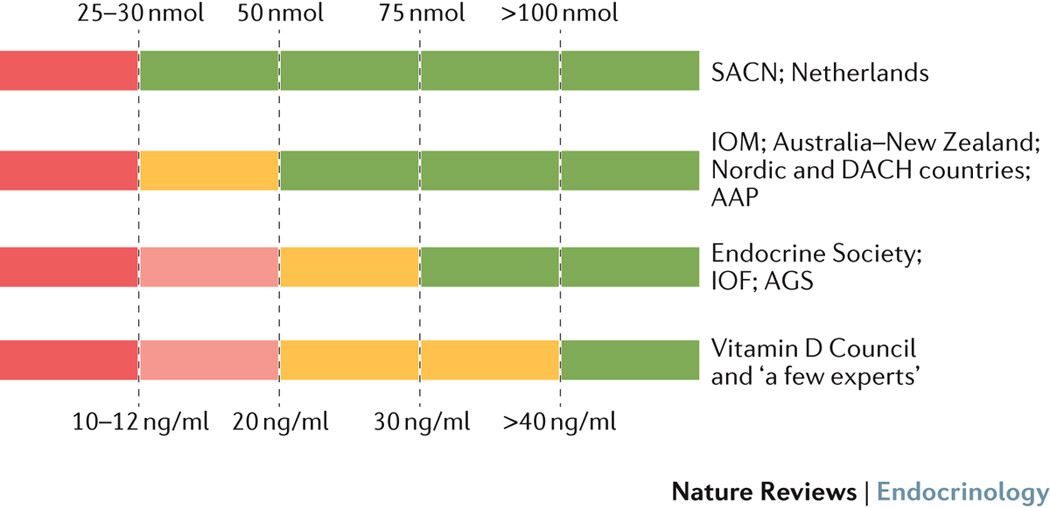
\includegraphics[width=0.8\textwidth]{
        figures/Bouillon.2017.comparative-Recommendations_for_interpreting_serum_levels_of_25OHD.jpg
    }
    \caption[Comparaison de l'interprétation des seuils de déficience en vitamine
    D.]{\textbf{Comparaison de l'interprétation des seuils de déficience en
    vitamine D }\autocite{Bouillon.2017.comparative}.}
    \label{fig-vd-comparison}
\end{figure}

\section{Associations observées dans les études
observationnelles}\label{associations-observuxe9es-dans-les-uxe9tudes-observationnelles}

La majorité des méta-analyses des études observationnelles rapportent
une corrélation inverse entre la sévérité de la maladie et la
concentration en vitamine D (\Cref{tab:meta-analyses-obs}). En effet,
les patients COVID-19 sévères ont une concentration en vitamine D
souvent inférieure à 20 ng/mL, où plusieurs méta-analyses et revues
systématiques rapportent une déficience sévère (\textless{} 10-12 ng/mL)
à un risque accru de sévérité
\autocite{Contreras-Bolívar.2023, Borsche.2021,
Crafa.2021, DEcclesiis.2022, Pal.2022, Hariyanto.2022, Ghelani.2021}.
Similairement, l'étude écologique de \textcite{Ilie.2020} sur les pays
européens rapporte une corrélation inverse entre la concentration sévère
de vitamine D (\textless{} 12 ng/mL) avec une moyenne de 22 ng/mL et la
morbidité et la mortalité. Il a été également observé que la population
âgée de l'Espagne, l'Italie et la Suisse était en déficience sévère de
vitamine D. De même, l'étude de rétrospective sur une cohorte des
patients aux Etats-Unis de \textcite{Gibbons.2022} observe que la
supplémentation en vitamine D diminue le risque de mortalité de 33 \%
sur une période de 30 jours et le risque d'infection de 20 \%. Les
auteurs notent qu'après stratification des patients en fonction de leur
concentration en vitamine D, les patients entre 0-19 ng/mL observent la
plus grande diminution en infection par la COVID-19 après
supplémentation. Une étude d'un centre hospitalier rapporte que chez le
groupe de patients considéré vitamine D déficient (\textless{} 12 ng/mL)
contre non déficient (\textgreater{} 12 ng/mL), il existe une
association entre la déficience de vitamine D et le risque de
ventilation mécanique invasive et de mortalité (\ac{HR} = 6,12 et 14,73
respectivement) \autocite{Radujkovic.2020}.

Les patients hospitalisés présentent fréquemment des concentrations en
vitamine D critiquement basses comparés à la population générale.
\textcite{Hernández.2020} rapporte dans une étude cas-contrôle
rétrospective que parmi les 197 patients, 82,2 \% des patients étaient
en déficience (13,8 \pm ~7,2 ng/mL contre 20,9 \pm ~7,4 ng/mL). De même,
l'étude prospective de \textcite{Campi.2021} a étudié les niveaux de
vitamine D et d'IL-6 lors de l'admission chez 103 patients positif au
COVID-19 contre 206 sujets contrôles, et a constaté une concentration
plus faible chez les patients sévères (18,2 \pm ~11,4 ng/mL) contre les
patients légèrement symptomatiques ou contrôles (30,3 ± 8,5 ng/mL et
25,4 ± 9,4 ng/mL, respectivement). La \Cref{fig-vd-covid-deficiency}
illustre la proportion croissante de patient déficient en vitamine D en
fonction de la sévérité des symptômes à la COVID-19. Le niveau de
vitamine D est corrélé inversement au taux d'IL-6 et de mortalité
indépendamment des autres facteurs confondants.

\begin{figure}

\centering{

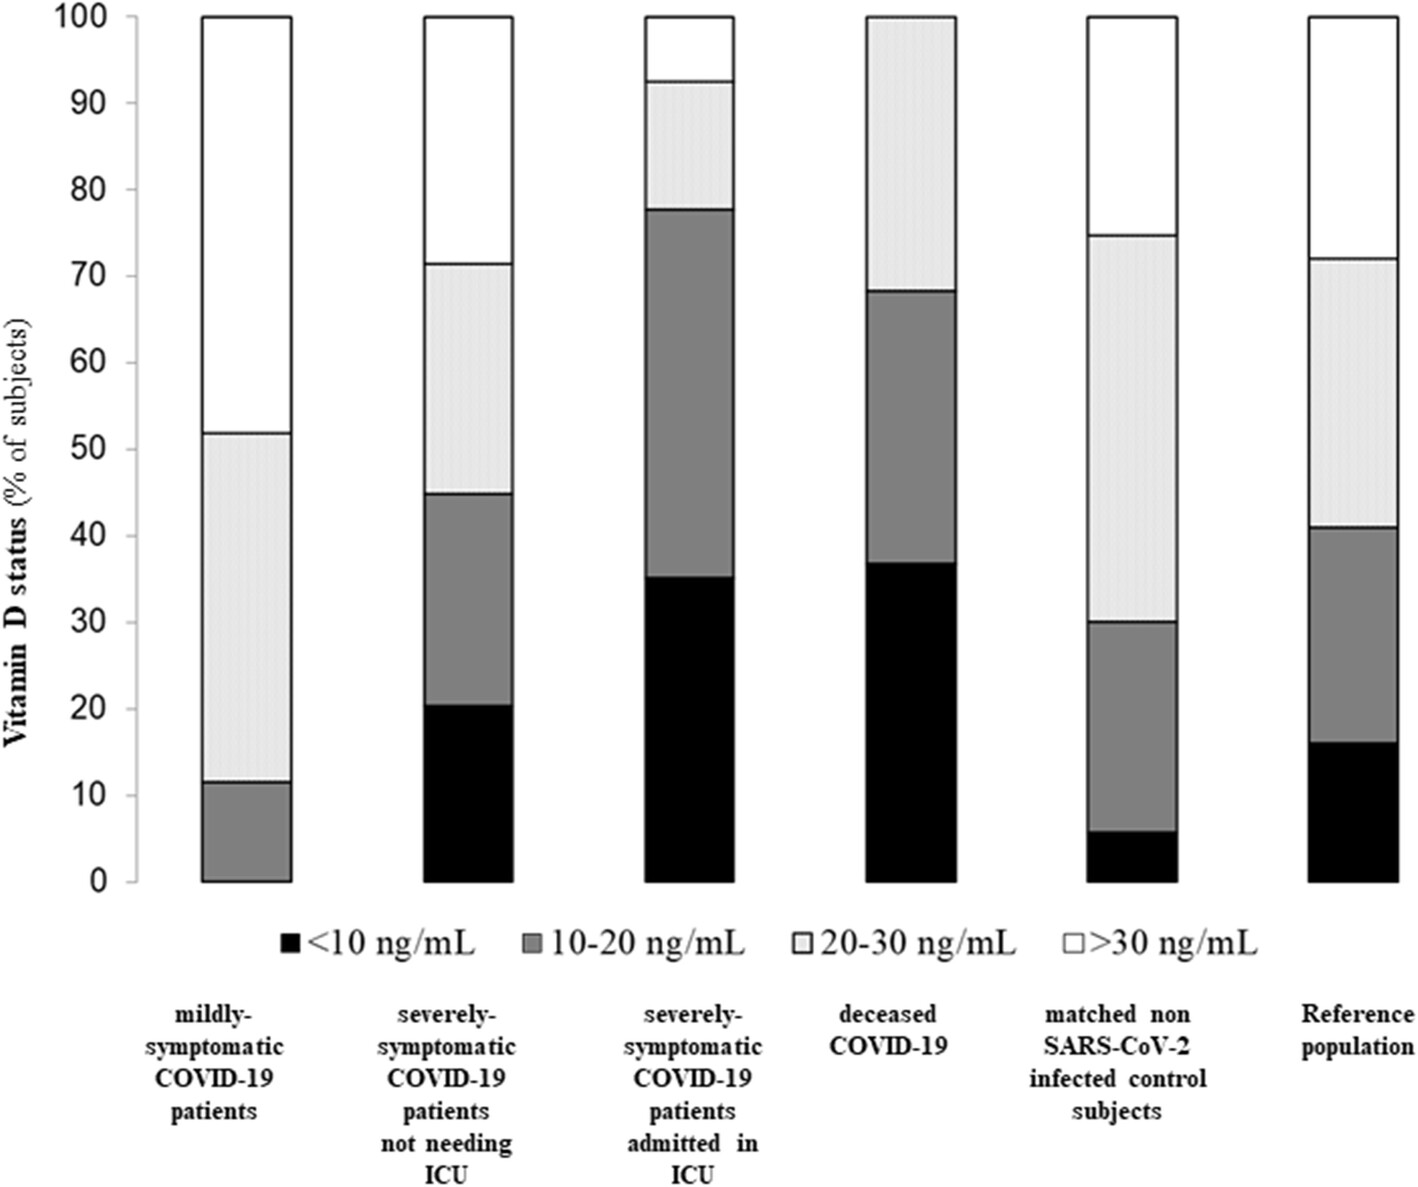
\includegraphics{figures/Campi.2021-Prevalence_rates_of_vitamin_D_insufficiency_or_deficiency.jpg}

}

\caption[Taux de prévalence de l'insuffisance ou de la carence en
vitamine D.]{\label{fig-vd-covid-deficiency}\textbf{Taux de prévalence
de l'insuffisance ou de la carence en vitamine D}
\autocite{Campi.2021}.}

\end{figure}%

Cette association n'est pas systématiquement retrouvée entre les études,
où certaines ne trouvent pas d'association entre la concentration en
vitamine D et la sévérité de la maladie, ou bien la mortalité
\autocite{Hernández.2020,Jevalikar.2021,Cereda.2021,Murai.2021}. Bien
qu'aucune association générale n'ait été trouvée entre la sévérité et la
déficience et la vitamine D par \textcite{Hernández.2020}, il est
intéressant de noter qu'une relation inverse a été observée avec la
ferritine (\emph{P} = 0,013) et la CRP (\emph{P} = 0,027) et le taux de
vitamine D, avec une plus grande prévalence de l'hypertension et de
maladies cardiovasculaires ainsi qu'une augmentation de la ferritine et
de la troponine et l'augmentation de la durée d'hospitalisation comparé
aux patients ayant un niveau de calcidiol \textgreater{} 20 ng/mL.

Dans une étude rétrospective menée en Espagne sur une cohorte de 108 343
patients, les auteurs de l'étude d'\textcite{Oristrell.2022} n'ont pas
trouvé d'association significative entre la supplémentation en vitamine
D et les résultats cliniques globaux. Cependant, les patients ayant des
niveaux de vitamine D supérieurs à 30 ng/mL ont montré une diminution de
la mortalité, de la sévérité de la maladie, et du risque d'infection.

En particulier, les trois méta-analyses effectuées par
\textcite{Kaya.2021} rapportent que les individus déficients en vitamine
D sont 1,64 (\(IC_{95\%} = [1,32 ; 2,04] ; P < 0,001\)) fois plus
susceptibles de contracter la COVID-19, 2,42 fois
(\(IC_{95\%} = [1,13 ; 5,18] ; P = 0,022\)) plus de chance de développer
une forme sévère, tandis que le niveau faible de vitamine D n'a pas eu
d'effet sur la mortalité
(\(OR = 1,64 ; IC_{95\%} = [0,53 ; 5,06] ; P = 0,390\)).

Globalement, les pays de l'hémisphère sud ont un taux de mortalité plus
bas que les pays de l'hémisphère nord \autocite{Contreras-Bolívar.2023},
tel que les Etats-Unis (68 par million) contre l'Australie (2 par
millions) \autocite{Bishop.2021}. Il existe des exceptions telles que
l'Espagne et l'Italie qui ont une plus grande mortalité, associé à une
prévalence de déficience en vitamine D plus importante, qui peuvent
s'expliquer par le biais de la préférence à l'ombre, et de la
pigmentation plus importante de la peau qui diminue la synthèse en
vitamine D. Les pays scandinaves ont une mortalité plus basse, associé à
une consommation plus fréquente d'huile de foie de morue ainsi que de
fortifications de laits et de laitages. La mortalité due au COVID-19 est
associé à des comorbidités telles que l'âge et des maladies chroniques,
qui sont également associés à une concentration plus basse de vitamine D
\autocite{Bishop.2021}. Certaines études observationnelles ne trouvent
pas d'association positive entre la supplémentation en vitamine D et la
diminution du risque de mortalité. Cependant, certaines études révèlent
une association lors de l'analyse sous-groupe concernant des patients
carencés en vitamine D, une association bénéfique lorsque les patients
possèdent une concentration \textgreater{} 30 ng/mL
\autocite{Oristrell.2022} ou bien certaines examinent des patients qui
ne sont pas en état déficitaire de vitamine D.

Les études écologiques rapportent également une différence de
concentration de vitamine D entre les patients COVID-19 positifs et
négatifs (10.8 nmol/L vs 20.8 nmol/L, \textcite{Baktash.2021}). En
effet, il existe une corrélation positive entre l'incidence de COVID-19
et le taux de déficience en vitamine D considéré comme \textless{} 20
ng/mL (R = 0.36), la fatalité (R = 0.40) et de mortalité (R = 0.38). Le
pourcentage médian de déficience de vitamine D est de 49 \%, allant de
13 \% pour le premier quintile à 65 \% pour le cinquième quintile
(indiquant que 23 pays sur les 46 analysés ont plus de 49 \% de
déficience à la vitamine D) \autocite{Mariani.2021}.

Parmi les études observationnelles, la méta-analyse de 32 études (n =
7771) par \textcite{Hopefl.2021} montre que les patients à niveau
suffisant de vitamine D possèdent des niveaux plus bas de CRP, IL-6,
ferritine, LDH, fibrinogène et D-dimères comparé au groupe de patients
déficients en vitamine D. Seul le paramètre analysé de sédimentation des
érythrocyte n'est pas différent entre les deux groupes.

La \Cref{tblr:meta-analyses-obs} résume l'opinion des méta-analyses et
études citées.

\begin{landscape}
\begin{longtblr}[
    theme = tinyfr,
    caption = {\textbf{Opinion des méta-analyses sur les études observationnelles concernant l'existence d'une relation entre la vitamine D et la COVID-19.} \acs{IC},  \acl{IC} ; \acs{MD}, \acl{MD} ; \acs{RCT}, \acl{RCT} ; \acs{RR}, \acl{RR} ; \acs{SMD}, \acl{SMD}.},
    entry = {Opinion des méta-analyses sur les études observationnelles concernant l'existence d'une relation entre la vitamine D et la COVID-19.},
    label = {tblr:meta-analyses-obs}
]{
    colspec = {l p{6cm} X},
    cells= {font = \small},
    row{1} = {font=\bfseries \small, halign=c},
    rowhead = 1
}

\toprule
Étude & Design et taille de l'échantillon & Opinion \\
\midrule


% June 2021
\textcite{Bassatne.2021} & Méta-analyse de 31 études observationnelles et 3 \ac{RCT} & Les auteurs notent une tendance positive entre la déficience (< 20 ng/mL) et l'augmentation de la mortalité, l'admission en soins intensifs, le recours à la ventilation mécanique invasive ou non et la positivité au SARS-CoV-2 parmi les études observationnelles. La moyenne sérique du taux de calcidiol est 5,9 ng/mL ($IC_{95\%} = [-9,5 ; -2,3]$) plus basse chez les patients COVID-19 comparés au groupe contrôle. Lorsque le seuil de déficience est augmenté à 30 ng/mL, le risque de mortalité et de positivité au SARS-CoV-2 est augmenté. Les auteurs notent la qualité très pauvre des études observationnelles et la certitude des preuve très basse. \\

\textcite{Crafa.2021} & Méta-analyse et revue systématique de 30 études. & Les
taux sériques de calcidiol sont significativement plus bas chez les patients
atteints d'une infection par le SARS-CoV-2 que chez les patients séronégatifs
($ MD = -3,99 ; IC_{95\%} = [-5,34 ; -2,64] ; P < 0,00001 ; I^2 = 95 \% $), et sont plus bas chez les patients en état sévère ($MD = -6,88 ; IC_{95\%} = [-9,74 ; -4,03] ; P < 0,00001 ; I^2 = 98\%$) et chez les patients décédés du COVID-19 ($MD -8,01 ; IC_{95\%} = [-12,50 ; -3,51] ; P = 0,0005 ; I^2 = 86 \%$]. Enfin, les patients déficients en vitamine D avaient un risque accru de développer une maladie sévère ($OR = 4,58 ; IC_{95\%} = [2,24 ; 9,35] ; P < 0,0001 ; I^2 = 84 \%$), mais pas de mortalité ($OR = 4,92 ; IC_{95\%} = [0,83 ; 29,31] ; P = 0,08 ; I^2 = 94\%$). \\

\textcite{Ghasemian.2021} & Méta-analyse et revue systématique de 23 études (n =
11 901) & 41 \% des patients COVID-19 sont déficients (< 20 ng/mL) en vitamine D
(moyenne de 20,3 ng/mL), 42 \% des patients ont un niveau insuffisant (20-30
ng/mL). Lors d'une déficience, les patients ont 3,3 fois plus de chance de
contracter la COVID-19 et 5 fois plus de chance de développer un COVID-19
sévère. Il n'existe pas d'association entre le statut en vitamine D et un plus
fort taux de mortalité. \\

\textcite{Jevalikar.2021} & Étude prospective observationnelle (n = 410). & 48,2
\% des 410 patients ont un taux de vitamine D \textless 20 ng/mL, mais les auteurs ne
retrouvent pas d'associations avec la sévérité, la mortalité, ou l'admission
hospitalière, le besoin en oxygénothérapie et ne trouvent pas de corrélation
avec les marqueurs inflammatoires (IL-6, CRP). \\

\textcite{Kaya.2021} & Méta-analyse de 21 études observationnelles (n = 205 869)
& La déficience (< 20 ng/mL) augmente le risque d'infection COVID-19 et risque
de maladie sévère. Les individus déficients ont 1,64 fois plus de chance de
contracter la COVID-19 et les patients < 20 ng/mL ont 2,42 fois plus de chance
de contracter une forme sévère de la maladie. Le statut bas en vitamine D n'a
pas d'effet sur la mortalité.\\

\textcite{Munshi.2021} & Méta-analyse de 6 études observationnelles (n = 376) &
Les patients COVID-19 ont une moyenne de 8,76 ng/mL. Les patients avec une
hypovitaminose D (moyenne = 8.79 ng/mL) ont un mauvais pronostic pour les
patients COVID-19 ($ SMD = -0,58, IC_{95\%} = [−0,83 ; −0,34], P < 0,001 $). \\

\textcite{Petrelli.2021} & Méta-analyse de 43 études observationnelles (n = 612
601) & La carence en vitamine D est associée à une aggravation de la gravité et
à une mortalité plus élevée que chez les patients non carencés ($OR = 2,6 ;
IC_{95\%} = [1,84 ; 3,67] ; P < 0,01 $ et $OR = 1,22 ;  IC_{95\%} = [1,04 ; 1,43] ; P < 0,01$, respectivement). \\

% March 2021
\textcite{Teshome.2021} & Méta-analyse de 14 études pour analyse qualitative
dont 8 études pour analyse quantitative & L'analyse qualitative indique que les
patients déficients ont 80 \% plus de chance de contracter l'infection à la
COVID-19 ($OR = 1,80 ; IC_{95\%} = [1,72 ; 1,88]$). L'analyse sous-groupe révèle
que la chance d'être infecté est plus grande dans les études type cas-témoins
(OR = 1,81). \\

% April 2022
% Yes Readcube Papers use 2021 as year.
\textcite{Dissanayake.2021} & Méta-analyse de 72 études observationnelles & La carence en vitamine D augmente les chances de développer la COVID-19 ($OR = 1,46 ; IC_{95\%} = [1,28 ; 1,65] ; P < 0,0001 ; I^2 = 92\%$), une maladie grave ($OR = 1,90 ; IC_{95\%} = [1,52 ; 2,38] ; P < 0,0001 ; I^2 = 81\%$), et la mort ($OR = 2,07 ; IC_{95\%} = [1,28 ; 3,35] ; P = 0,003 ; I^2 = 73\%$). Les concentrations de calcidiol étaient plus faibles chez les personnes atteintes de COVID-19 que chez les témoins ($MD = -3,85 ng/mL ; IC_{95\%} = [-5,44 ; -2,26] ; P ≤ 0,0001$), chez les patients atteints de COVID-19 sévère par rapport aux témoins atteints de COVID-19 non sévère ($MD -4,84 ng/mL ; IC_{95\%} = [-7,32 ; -2,35] ; P = 0,0001]$) et chez les non-survivants par rapport aux survivants ($MD = -4,80 ng/mL ; IC_{95\%} = [-7,89 ; -1,71] ; P = 0,002$). \\

\textcite{Ben-Eltriki.2022} & Méta-analyse de 24 études observationnelles (n =
3637) &  Un faible statut en vitamine D était statistiquement associé à un
risque plus élevé de mortalité ($ RR = 1,60 ; IC_{95\%} = [1,10 ; 2,32] $), à un
risque plus élevé de développer une pneumonie sévère COVID-19 (RR = 1,50 ;
$ IC_{95\%} = [1,10 ; 2,05] $). Les patients COVID-19 ont une CRP et un taux
d'IL-6 supérieur aux patients \geq \ 30 ng/mL. \\

\textcite{Pal.2022} & Méta-analyse de 10 études observationnelles et 3 \ac{RCT}
(n = 2933) &  Les auteurs observent une réduction de la mortalité ($ OR = 0,41 ;
IC_{95\%} = [0,20 ; 0,81] ; P = 0,01 ; I^2 = 66 \% $, modèle random effects)
ainsi que des effets indésirables ($ OR = 0,27 ; IC_{95\%} = [0,08 ; 0,91] ; P =
0,03 ; I^2 = 80 \% $, modèle random-effects). Les auteurs notent que la plupart
des études analysés ne rapportent pas les estimations de risques ajustés pour
les résultats cliniques après ajustement des facteurs de confusion potentiels.
\\

\bottomrule
\end{longtblr}
\end{landscape}

De manière intéressante, \textcite{Pal.2021} notent l'existence d'une
forte prévalence d'hypocalcémie chez les patients COVID-19 à symptôme
léger. et suggèrent que cela implique probablement que l'hypocalcémie
est intrinsèque à la maladie. Ce déséquilibre pourrait être dû à la
perturbation des niveaux de \ac{PTH} et/ou de calcidiol, ou bien être dû
à des niveaux d'acide gras élevés qui peuvent se lier au calcium,
causant l'hypocalcémie.

\section{Effets des interventions thérapeutiques dans la prévention et
le traitement de la
COVID-19}\label{effets-des-interventions-thuxe9rapeutiques-dans-la-pruxe9vention-et-le-traitement-de-la-covid-19}

Globalement, les méta-analyses rapportent une hétérogénéité notable des
essais cliniques ce qui rend les informations moins précises, et plus
difficiles à interpréter, comme par exemple concernant le jour de la
dose d'admission, la dose administrée Il existe de plus une part
d'études rapportant des résultats contradictoires. Selon
\textcite{Pal.2022}, il convient de noter que la plupart de ces études
n'ont pas rapporté d'estimations de risque ajustées pour les résultats
cliniques après ajustement des facteurs de confusion potentiels.

La vitamine D est indépendamment associée à la mortalité de la COVID-19
après ajustement du facteur confondant de la graisse viscérale d'après
\textcite{Vanegas-Cedillo.2022} . \textcite{Borsche.2021}, après
ajustement pour les facteurs confondants, arrive à la conclusion que
seul l'âge et la vitamine D sont associés à la mortalité de la COVID-19.

Malgré des essais cliniques contradictoires, il existe une proportion de
méta-analyses et d'études cliniques qui rapportent des effets bénéfiques
de la vitamine D dans la prévention et le traitement de la COVID-19
\autocite{Pal.2022}.

\subsection{Etudes cliniques}\label{etudes-cliniques}

Il existe plusieurs phases de progression de la sévérité de la COVID-19.
L'Organisation Mondiale de la Santé a défini une classification des
phases en fonction de leur sévérité \autocite{WHO.2023.org,Agarwal.2020}
:

\begin{itemize}
\tightlist
\item
  Phase symptomatique légère: Fièvre, toux, fatigue, anorexie,
  essoufflement, myalgie, anosmie, agueusie. Symptômes non spécifiques:
  maux de gorge, congestion nasale, maux de tête, diarrhée, nausées et
  vomissements
\item
  Phase modérée : Définie comme l'absence de critères sévères ou
  critiques. Pneumonie (fièvre, toux, dyspnée, hyperventilation),
  \ac{SpO2} \textgreater{} 90 \%
\item
  Phase sévère : Pneumonie, sepsis, \ac{SpO2} \textless{} 90 \%,
  fréquence respiratoire \textgreater{} 30/min
\item
  Phase critique: \ac{SDRA}, sepsis, choc septique, thrombose aiguë
  nécessitant une ventilation mécanique ou traitement par vasopresseurs
  en unité de soins intensifs.
\end{itemize}

\subsubsection{Etudes en phase hospitalière (visée
curative)}\label{etudes-en-phase-hospitaliuxe8re-visuxe9e-curative}

Dans la majorité des études évaluant l'efficacité curative de la
vitamine D, les patients sont déjà infectés par le \ac{SARS-CoV-2} et
symptomatiques au moment de l'inclusion. Une dose unique ou répétée de
vitamine D leur est administrée dès leur admission à l'hôpital.
L'opinion des méta-analyses sur les essais cliniques est résumée dans la
\Cref{tblr:meta-analyses-rct}.

\begin{landscape}
\begin{longtblr}[
    theme = tinyfr,
    caption = {\textbf{Opinion des méta-analyses sur les essais cliniques concernant l'impact de la supplémentation en vitamine D sur la mortalité, la sévérité et/ou l'admission en soins intensifs.} \acs{HR}, \acl{HR} ; \acs{IC}, \acl{IC} ; \acs{OR}, \acl{OR} ; \acs{RCT}, \acl{RCT} ; \acs{RR}, \acl{RR}.},
    entry = {Opinion des méta-analyses sur les essais cliniques concernant l'impact de la supplémentation en vitamine D sur la mortalité, la sévérité et/ou l'admission en soins intensifs.},
    label = {tblr:meta-analyses-rct}
]{
    colspec = {l p{6cm} X},
    row{1} = {font=\bfseries \small, halign=c},
    rowhead = 1,
}

\toprule
\textbf{Étude} & \textbf{Design et taille de l'échantillon} & \textbf{Opinion} \\
\midrule

% Table content goes here

% October 2021
\textcite{Borsche.2021} & Méta-analyse et revue systématique de 8 \ac{RCT} (n =
114 415) et 1 population d'étude. & Forte corrélation inverse de mortalité avec
le taux de vitamine D à la fois pour la population d'étude et l'ensemble des RCT
analysés, avec un taux de mortalité théorique proche de zéro obtenu à 50 ng/mL
($r(32) = −0,3989 ; P = 0,0194$). \\

% \textcite{Murai.2021} & Essai clinique randomisé (n = 120) & L'essai clinique
% ne recommande pas la supplémentation en vitamine D. Dose unique de 200 000 UI de
% vitamine D~3~ vs placebo, n = 120. Pas de différence significative en terme de
% durée d'hospitalisation, de mortalité, d'admission aux urgences ou de
% ventilation mécanique. \\
% Note: Not meta-analysis, skipped

% January 2022
\textcite{Pal.2022} & Méta-analyse de 10 études observationnelles et 3 \ac{RCT}
(n = 2933) & L'analyse étant confondues, il n'est pas possible de séparer les
types d'études. Les auteurs observent une réduction de la mortalité ($OR = 0,41 ;
IC_{95\%} = [0,20 ; 0,81] ; P = 0,01 ; I^2 = 66 \%$, modèle random effects)
ainsi que des effets indésirables ($OR = 0,27 ; IC_{95\%} = [0,08 ; 0,91] ; P =
0,03 ; I^2 = 80 \%$, modèle random-effects). Les auteurs notent que la plupart
des études analysés ne rapportent pas les estimations de risques ajustés pour
les résultats cliniques après ajustement des facteurs de confusion potentiels.
\\

% March 2022
\textcite{Hariyanto.2022} & Méta-analyse de 11 RCT. & L'analyse suggère que la
supplémentation en vitamine D est associée à une réduction du taux d'admission
en unité de soins intensifs ($OR = 0,27 ; IC_{95\%} = [0,09 ; 0,76] ; P =
0,010$), à une réduction du besoin de ventilation mécanique ($OR = 0,34 ;
IC_{95\%} = [0,16 ; 0,72] ; P = 0,005$) et à une réduction de la mortalité due à
la COVID-19 ($OR = 0,37 ; IC_{95 \%} = [0,21 ; 0,66] ; P < 0,001$). L'analyse
méta-régression impacte l'association entre la supplémentation en vitamine D et
la mortalité, mais pas le genre, l'hypertension, le diabète ou l'usage de
corticostéroïdes. \\


% September 2023
\textcite{Meng.2023} & Méta-analyse de 23 RCT & Les effets préventifs de la supplémentation en vitamine D sont inconclusifs (4 essais cliniques analysés). Les auteurs observent une réduction de l'admission aux soins intensifs ($RR = 0,63 ; IC_{95\%} = [0,44 ; 0,89]$) et le recours à la ventilation mécanique ($RR = 0,58 ; IC_{95\%} = [0,39 ; 0,84]$). L'analyse ne retrouve pas d'effet sur la mortalité, cependant l'analyse sous-groupe révèle que la supplémentation en vitamine D est associée à une réduction de la mortalité chez les patients déficients ($RR = 0,76 ; IC_{95\%} = [0,58 ; 0,98]$). \\

% February 2024
\textcite{Jamilian.2024} & Méta-analyse parapluie de 13 méta-analyse comprenant
9 études synthétisant les données sur les études observationnelles et 4 sur les
essais cliniques randomisés & Les résultats révèlent que le statut en vitamine D
et la supplémentation réduit la mortalité, retrouvé dans les études interventionnelles
($ES = 0,42 ; IC_{95\%} = [0,10 ; 0,75] ; P < 0,001 ; I^2 = 20,4 \% ; P = 0,285$) et
observationnelles (déficience augmente la mortalité : $ES = 1,99 ; IC_{95\%} = [1,37 ; 2,62] ; P < 0,001 ; I^2 = 00,0\% ; P = 0,944$), tandis que la déficience augmente la
sévérité ($ES = 1,77; IC_{95\%} = [1,45 ; 2,10] ; P < 0,001 ; I^2 = 00,0\%, P = 0,463$) et le risque d'infection ($ES = 1,64 ; IC_{95\%} = [1,40 ; 1,88] ; P < 0,001 ; I^2 = 67,3 \%, P = 0,027$). L'analyse ne retrouve pas d'association entre le sérum et le statut positif de COVID-19. \\

% March 2024
\textcite{Zhong.2024} & Méta-analyse de 5 RCT (n = 11 901) & L'analyse
n'a pas trouvé de bénéfice d'une forte dose de vitamine D (définie comme une
dose unique de ≥ 100 000 UI ou une dose quotidienne de ≥ 10 000 UI atteignant une
dose totale de ≥ 100 000 UI) pour la mortalité ni l'admission en soins
intensifs, incluant l'analyse sous-groupe des patients déficients.\\

% May 2024
\textcite{Yang.2024} & Méta-analyse de 19 RCT. & Dans le sous-groupe sévère, l'analyse montre des effets bénéfiques concernant l'admission en soins intensifs ($OR 0,43, IC_{95\%} 0,23, 0,80 ; P = 0,008$), la ventilation mécanique ($OR 0,44, IC_{95\%} = [0,27 ; 0,72] ; P = 0,001$) et la durée d'hospitalisation ($SMD -0,49, IC_{95\%} = [0,92 ; -0,06] ; P = 0,027$). Dans le sous-groupe administration de la vitamine D, l'analyse montre des bénéfiques concernant l'admission en soins intensifs ($OR 0,39, IC_{95\%} = [0,16 ; 0,97] ; P = 0,044$), de la ventilation mécanique ($OR 0,18, IC_{95\%} = [0,07 ; 0,46] ; P = 0,000$) et de l'admission en soins intensifs ($SMD -0,50, IC_{95\%} -0,96, -0,04 ; P = 0,000$). Ces effets sont plus prononcés chez des patients supplémentés avec de multiples doses de vitamine D plutôt qu'une dose unique. Bien que le résultat de la mortalité n'ait pas montré d'effet statistiquement significatif, les auteurs notent qu'il indique une tendance à la baisse ($OR 0,87, IC_{95\%} 0,63, 1,12 ; P > 0,05$). Les résultats des marqueurs inflammatoires n'ont révélé aucune différence statistique. \\

% May 2024
\textcite{Sobczak.2024} & Méta-analyse de 13 \ac{RCT} & La méta-analyse montre un effet bénéfique de la supplémentation en vitamine D sur la mortalité ($RR = 0,56 ; IC_{95\%} = [0,34 ; 0,91] ; P = 0,02 ; I^2 = 0\%$), ainsi que pour la diminution du taux d'admission en soins intensifs ($ RR = 0,73 ; IC_{95\%} = [0,57 ; 0,95] ; P = 0,02, I^2 = 19,6 \% $)


\end{longtblr}
\end{landscape}

La méta-analyses parapluie de \textcite{Jamilian.2024} a analysé le rôle
de la vitamine D concernant la mortalité, le risque d'infection, la
sévérité de la maladie, le risque d'admission en soins intensifs et le
taux de ventilation mécanique. Les résultats révèlent que le statut en
vitamine D et la supplémentation réduit la mortalité, tandis que la
déficience augmente la sévérité et le risque d'infection, retrouvés dans
les études interventionnelles et observationnelles.

La méta-analyse de \textcite{Borsche.2021} rapporte une forte
corrélation inverse de mortalité avec le taux de vitamine D. Les auteurs
suggèrent également que les taux de vitamine D sont sans dangers en
prenant en compte les besoins en vitamine K\textsubscript{2} ; certains
répondeurs faibles à la vitamine D devraient avoir une concentration
augmentée à 75 ou 100 ng/mL pour avoir un effet similaire aux répondeurs
modérés. L'analyse des 8 études rapportent une médiane de 23,2 ng/mL.
Les régressions mathématiques de deux bases de données séparées montrent
que le taux de mortalité diminue à partir de 30 ng/mL, et un seuil de 50
ng/mL serait optimal pour diminuer la mortalité liée à la COVID-19.

La concentration de vitamine D dans le sang semble correspondre à
certains seuils d'efficacité, en-dessous desquels la vitamine D n'exerce
pas d'effet immunitaire notable. Par exemple, l'étude \emph{in vitro} de
\textcite{Zhang.2012} a démontré une inhibition de la production de
cytokines, notamment de l'\ac{IL-6}, à partir d'un taux de 30 ng/mL de
vitamine D, avec des tests effectués jusqu'à 70 ng/mL. L'inhibition
maximale a été observée à 50 ng/mL, sans effet inhibiteur supplémentaire
au-delà de ce seuil, même à 70 ng/mL.

L'étude de \textcite{Kaufman.2020}, portant sur 191 779 patients, a
révélé que 39 190 d'entre eux (12,5 \%) étaient positifs au COVID-19
avec un taux de vitamine D inférieur à 20 ng/mL, 27 870 patients (8,5
\%) avec un taux entre 30 et 34 ng/mL, et 12 321 patients positifs avec
un taux supérieur ou égal à 55 ng/mL. Le taux minimal d'infection a été
observé chez les patients avec un niveau de vitamine D de 55 ng/mL.

Ces études expliquent l'intention des études et le rationnel clinique
derrière la supplémentation en vitamine D visant à obtenir ces seuils
jugés optimaux pour la réduction de la mortalité ainsi que du risque
d'infection et de sévérité de la maladie.

En ce qui concerne certains indicateurs biologiques intéressants,
l'administration de vitamine D (3000-6000 UI/jour pendant 2 mois) est
corrélée à une diminution du ratio neutrophiles/lymphocytes
périphériques, un indicateur fonctionnel lié à une réduction de la
mortalité et du passage aux soins intensifs \autocite{Maghbooli.2021}.

Il a été observé que le rapport entre le peptide LL-37 et le nombre
total de leucocytes sériques chez les patients atteints de COVID-19 est
corrélé avec la sévérité. Il existe une corrélation entre le \ac{CRP},
\ac{IL-6}, \ac{PCT}, compte leucocytaire, \ac{LDH} et sévérité de la
maladie \autocite{Keutmann.2022}. Des niveaux sériques plus faibles de
LL-37 sont associés à la gravité de la maladie et à la durée du séjour à
l'hôpital \autocite{Keutmann.2022} et il a été observé que les niveaux
de calcidiol sont directement corrélés aux niveaux de LL-37 chez les
patients en sepsis \autocite{Cutuli.2024}.

Dans l'étude ancillaire post-hoc d'un essai clinique randomisé,
\textcite{Fernandes.2022} observent une différence du taux de GM-CSF
avec un niveau plus bas chez les patients supplémentés avec une dose
bolus de 200 000 UI par rapport au bras contrôle. La surexpression de
GM-CSF est associé à un état inflammatoire sévère et due à une réponse
autocrine positive et à une boucle de rétroaction positive.

\subsubsection{Etudes en phase
réanimation}\label{etudes-en-phase-ruxe9animation}

La déficience en soin intensif est généralement définie comme une
concentration de calcidiol (25(OH)D) inférieure à 12 ng/mL, tandis que
la déficience est établie par l'\ac{IOM} comme inférieure à 20 ng/mL
\autocite{Cutuli.2024}.

Dans un contexte de soins intensifs hors COVID-19, il a été rapporté que
40 à 70 \% des patients en réanimation présentent une carence en
vitamine D. Les études observationnelles indiquent qu'une concentration
de vitamine D inférieure à 15 ng/mL est prédictive d'un risque accru de
sepsis et de mortalité. Parmi les patients carencés, 93,5 \% présentent
une déficience, dont 53,3 \% affichent des taux extrêmement bas,
inférieurs à 7 ng/mL. Les méta-analyses révèlent que de faibles niveaux
de vitamine D sont indépendamment associés à une mortalité plus élevée.
Plus spécifiquement, l'analyse par sous-groupes montre que seule une
carence en vitamine D inférieure à 10 ng/mL est corrélée à une
augmentation de la mortalité, tandis que cette association n'est pas
observée pour des concentrations plus élevées \autocite{Cutuli.2024}.

Deux essais cliniques notables à large échelle ont examiné le rôle de la
vitamine D en soins intensifs (hors COVID-19), à savoir les études
\emph{VITdAL-ICU} et \emph{VIOLET.} Le design de \emph{VITdAL-ICU}
(phase 2) comprend une dose bolus de vitamine D de 540 000 UI suivie
d'une dose mensuelle de maintenance de 90 000 UI pour 5 mois. Bien
qu'aucune conclusion positive n'ait été tirée en terme de résultats
cliniques, l'analyse sous-groupe avec de patients déficients
(\textless{} 12 ng/mL) révèle une réduction de la mortalité dans le
groupe traité à la vitamine D par rapport au placebo (28,6 \% vs 46,1
\%) \autocite{Cutuli.2024}. L'étude \emph{VIOLET} (phase 3) portant sur
1358 patients avec une dose de charge de 540 000 UI avant admission aux
soins intensifs et sans dose de maintien, a été interrompue
prématurément pour futilité. De plus les deux études présentent un
faible taux de sepsis (7,7 \% et 33,3 \% respectivement), empêchant une
analyse statistique adéquate. Trois autres études, analysées par
\textcite{Cutuli.2024}, incluaient un effectif plus réduit et n'ont pas
fourni de résultats concluants. Selon les auteurs, des essais cliniques
spécialisés de grande envergure sont nécessaires pour répondre au rôle
de la vitamine D pour contrôler l'infection et améliorer le
dysfonctionnement inflammatoire et la septicémie.

Une méta-analyse de cinq \ac{RCT} par \textcite{Argano.2023} a examiné
la mortalité et les admissions en soins intensifs des patients en état
sévère de COVID-19, évaluant le risque de biais selon la méthodologie
Cochrane ROB 2, ainsi qu'une analyse de type \ac{TSA}
\autocite{Kang.2021}. Les résultats montrent que l'administration de
vitamine D est associée à une réduction significative de la mortalité et
des admissions en soins intensifs, avec des \ac{SMD} de 0,49
(IC\textsubscript{95\%} = {[}0,34 ; 0,72{]}) et 0,28
(IC\textsubscript{95\%} = {[}0,20 ; 0,39{]}), respectivement. L'analyse
\ac{TSA} suggère que le nombre de patients inclus est suffisant pour
conclure à une réduction des admissions en soins intensifs, mais que
l'effet protecteur de la vitamine D sur la mortalité nécessite des
recherches supplémentaires.

Similairement, la méta-analyse de \textcite{Sîrbu.2023} sur 13 essais
cliniques randomisés montre des résultats cliniques améliorés pour des
patients traités à la vitamine D par rapport à ceux recevant un placebo
ou ne recevant pas de vitamine D (\ac{RR} = 0,63 ;
IC\textsubscript{95\%} = {[}0.41 ; 0.99{]} ; \emph{P} = 0,04 ; un risque
relatif plus petit favorise la vitamine D), mais n'observe pas de
résultat statistiquement différent en ce qui concerne la mortalité
(\ac{RR} = 0,93 ; IC\textsubscript{95\%} = {[}0,57 ; 1,52{]}, \emph{P} =
0,78).

Des différences de population de lymphocytes T ont été observé chez les
patients carencés en vitamine D. L'étude de
\textcite{Karonova.2022.pharmaceuticals} menée auprès de 321 patients a
révélé une prévalence significative de formes sévères chez ceux
présentant une carence en vitamine D. L'analyse par courbe ROC a
identifié un seuil critique de 11,4 ng/mL, associé à une mortalité
accrue. En dessous de ce niveau, une diminution des cellules T
CD3\textsuperscript{+} CD4\textsuperscript{+} a été observée, ainsi
qu'une réduction des cellules T folliculaires auxiliaires dans les deux
groupes étudiés. En revanche, chez les patients dont le niveau de
vitamine D dépassait 11,4 ng/mL, une augmentation des cellules T mémoire
centrales de type Th2 et une diminution des cellules T mémoire centrales
de type Th17 est observé.

La récente méta-analyse parapluie de \textcite{Jamilian.2024} publiée en
avril 2024 inclut deux méta-analyses s'intéressant au bénéfice de la
vitamine D lors des soins intensifs, mais rapporte que les résultats
sont contradictoires : la méta-analyse de \textcite{Rawat.2021} ne
réduit pas les taux d'admissions en soins intensifs, tandis que
\textcite{Shah.2021} rapportent un taux plus faible d'admission comparé
aux patients sans supplémentations. \textcite{Jamilian.2024} sur la base
de \textcite{Rawat.2021} et \textcite{Bassatne.2021} (étude
\emph{VIVID}) ne rapportent également pas de bénéfice de la vitamine D
sur le sérum ou la réduction de ventilation mécanique invasive ou
non-invasive. Les auteurs notent le manque d'études évaluant la vitamine
D dans le contexte de la COVID-19 en soins intensifs.

\section{Discussion}\label{discussion}

\subsection{Méthodologie des
études}\label{muxe9thodologie-des-uxe9tudes}

Il existe de multiples méta-analyses, et essais cliniques randomisés,
montrant une efficacité de la vitamine D en ce qui concerne un usage en
prévention, curatif ou même dans un cadre critique nécessitant le
passage en unité de soin intensif. Les études dégagent plusieurs points
notables : la supplémentation en vitamine D conduit à une réduction de
la mortalité et la déficience en vitamine D est associée à une
augmentation de la mortalité et sévérité de la maladie et du risque
d'infection parmi les patients, ainsi qu'un pronostic défavorable. Ces
informations sont notamment appuyées par la méta-analyse parapluie de
\textcite{Jamilian.2024}. En ce qui concerne les patients en soins
intensifs, la vitamine D peut être associée à une réduction de la
mortalité et du taux d'admission, mais à cause du nombre réduit
d'études, la conclusion reste incertaine.

Malgré cela, il existe également des études montrant l'absence d'effet
de la vitamine D ce qui rend incertain la place de la vitamine D dans
l'arsenal thérapeutique de la COVID-19. Les études présentent une grande
variabilité concernant la méthodologie, la dose employée, et le moment
de l'administration de la vitamine D, ce qui augmente l'hétérogénéité
des résultats et l'incertitude de l'efficacité de la vitamine D. Même
lors des essais cliniques à grand nombre de patients, les résultats ne
sont pas tout le temps positifs. La méta-analyse de
\textcite{Zhong.2024} sur 5 essais cliniques ne supporte pas l'usage
d'une dose unique élevée de vitamine D dans un cadre curatif.

L'administration de vitamine D à visée curative pour une dose de 5000
UI/j est trop lente pour élever la concentration plasmatique de
calcidiol car la métabolisation de la vitamine D nécessite plusieurs
mois avant d'atteindre une concentration supérieure à 30 ng/mL
\autocite{Mocanu.2009}. Ainsi \textcite{Wimalawansa.2022} propose une
dose de charge élevée de vitamine D ou bien une dose bolus de calcidiol
oral qui serait rapidement absorbée par l'organisme, afin de pouvoir
rapidement élever la concentration de calcidiol à atteindre en quelques
jours ou heures respectivement. Une dose bolus de 100 000 UI est
suffisante pour atteindre des doses \textgreater20 ng/mL mais une dose
de 300 000 UI est nécessaire pour atteindre une concentration
\textgreater{} 30 ng/mL de calcidiol \autocite{Kearns.2014}

L'essai clinique de \textcite{Murai.2021}, considéré comme de bonne
qualité méthodologique par \textcite{Annweiler.2021} et
\textcite{Argano.2023}, selon les lignes directrices de
\textcite{Heaney.2014} : en effet, le raisonnement classique de la
supplémentation en vitamine D n'est pas équivalent à d'autres
médicaments, car les suppléments ne sont pas la seule source de vitamine
D, et de plus, il n'y a pas de relation dose-dépendante (?). L'étude de
\textcite{Murai.2021} échappe à 5 pièges de méthodologies des \acp{RCT}
: 1) Dose de charge pour remplir le stockage 2) Pas de traitement long
terme pour maintenir le taux de vitamine D 3) L'adhérence au traitement
est élevée 4) L'augmentation de la concentration de vitamine D est
vérifiée après supplémentation 5) Il est peu probable que le groupe de
contrôle ne reçoit pas de supplémentation en vitamine D car il est
hospitalisé par la même unité de recherche.

Selon \textcite{Leaf.2021} et \textcite{Annweiler.2021}, l'étude de
\textcite{Murai.2021} n'a pas suffisamment de puissance, et les patients
avec sévérité grave de la maladie sont exclus, ce qui pourrait expliquer
l'absence de différence significative entre les groupes. Seul la moitié
des patients sont déficients \textless20 ng/mL et seul un quart est en
déficience sévère \textless12 ng/mL. De plus, l'utilisation de la
longueur de séjour à l'hôpital comme critère principal est critiquable,
pouvant être influencée par d'autres facteurs comme le soutien social
disponible au domicile, et ne reflétant pas la sévérité de la maladie
\autocite{Annweiler.2021}, il aurait été préférable d'utiliser d'autres
critères de mesure de la mortalité, ou de la sévérité du COVID-19.

\textcite{Heaney.2014} propose des lignes directrices méthodologiques
concernant les essais cliniques pour les nutriments, où la méthodologie
actuelle est adaptée pour les médicaments pharmaceutiques mais inadaptée
pour les nutriments car les sources d'apports du nutriments sont
diverses et que la relation dose-réponse entre la dose et un objectif de
santé est non linéaire \autocite{Grant.2022.nutrients}. Les essais
cliniques devraient être basés sur la concentration en calcidiol
plasmatique initiale et celle à atteindre et non pas en dose de vitamine
D étant donné la grande hétérogénéité observée entre l'administration
d'une dose de vitamine D et la concentration plasmatique obtenue
\autocite{Grant.2022.nutrients}.

Selon \textcite{Grant.2022.nutrients}, les \ac{RCT} sur la vitamine D
dans un contexte général ont échoué car elles se sont concentrées sur la
dose administrée plutôt que sur la concentration du nutriment. Cela a
conduit à l'administration de doses faibles de vitamine D, insuffisantes
pour atteindre la concentration désirée. De plus, ces essais ont inclus
des patients dont le statut en vitamine D (calcidiol) dépassait celui de
la population moyenne, ignorant qu'il existe potentiellement différents
niveaux de concentration pour obtenir les bénéfices recherchés. Les
\ac{RCT} analysent les résultats de manière limitée, ne tenant pas
compte des effets non linéaires de la vitamine D ni de la forte variance
des dosages \autocite{Grant.2022,Grant.2018}. En effet, l'hétérogénéité
de la relation dose-réponse non linéaire est additionnellement illustrée
par les polymorphismes génétiques associés au CYP24A1, CYP2R1 et GC
\autocite{Grant.2018}, ainsi que la variabilité interindividuelle de la
réponse à la vitamine D \autocite{Vukić.2015}
(Section~\ref{sec-variabilite-reponse}). \textcite{Grant.2018} propose
ainsi une approche basée sur une concentration de calcidiol à
administrée à calculer en fonction des taux de base de la population
d'intérêt.

\subsection{Variabilité de la réponse à la vitamine
D}\label{sec-variabilite-reponse}

Selon le rationnel physiologique de l'effet de la vitamine D,
l'hétérogénéité des résultats peut s'expliquer par la dose
d'administration pouvant être insuffisante pour atteindre une dose jugée
optimale d'au moins 30 ng/mL et idéalement 50 ng/mL où le taux
d'infection et la mortalité seraient les plus basses
\autocite{Wimalawansa.2022,Kaufman.2020,Borsche.2021}. De plus comme la
vitamine D n'est pas un médicament mais un nutriment, il existe une
grande variabilité dans l'absorption de la vitamine D, qui peut être
influencée par la nutrition, et la variabilité d'absorption et de
distribution de la concentration de calcidiol qui est notamment
dépendante du poids \autocite{Ekwaru.2014}, ainsi que de la variabilité
génétique de réponse au VDR. Ainsi, \textcite{Vukić.2015} ont déterminé
qu'il existait deux groupes de répondeurs à la vitamine D en fonction du
nombre de pourcentage de gène activés, qui peut aller de 33 \% pour les
répondeurs les plus bas à 80 \% chez les forts répondeurs. La
variabilité de la réponse à la vitamine D entre patients est donc
potentiellement très élevée, et la concentration plasmatique atteinte
entre chaque patient pour une même dose de vitamine D peut être très
variable.

\textcite{Freitas.2021} \textcite{Onoja.2022}
\textcite{Delgado-Wicke.2024}

\subsection{Variabilité de la concentration de vitamine
D}\label{variabilituxe9-de-la-concentration-de-vitamine-d}

Mentionné par \textcite{Crafa.2021} : \textcite{Reijven.2020}
\textcite{Silva.2015} : Le calcidiol diminue lors d'une réponse aiguë à
une infection

\textcite{Giustina.2020} : Il est possible que la concentration faible
de calcidiol soit due à la réduction aiguë du \ac{DBP} circulant
\autocite{Christopher.2016}. Des doses élevées pourrait être nécessaire
dans le cadre des soins intensifs à cause de la sécrétion de cortisol
qui pourrait empêcher l'hydroxylation rénale et hépatique de la vitamine
D.

\subsection{Non-efficacité d'une dose bolus contre doses
multiples}\label{non-efficacituxe9-dune-dose-bolus-contre-doses-multiples}

La méta-analyse de \textcite{Meng.2023} note que deux revues concluent
que des doses de maintenance journalière de vitamine D est plus efficace
que des doses uniques pour réduire la mortalité, ce qui coïncide avec
leurs résultats. En effet, un essai clinique récent supplémentation en
vitamine D à bolus forte dose intermittente s'est retrouvé en échec face
à la prévention de, l'indication originale pour laquelle la vitamine D a
été découverte et utilisée \autocite{Crowe.2021}.
\textcite{Griffin.2021} notent que les méta-analyses de la
supplémentation en vitamine D chez d'autres pathogènes corroborent
l'efficacité à plus faible dose journalière plutôt que d'une dose bolus.

\textcite{Mazess.2021}

Les effets plus prononcés de l'administration de la vitamine D sont
retrouvés dans la méta-analyse de \textcite{Yang.2024}, cité dans la
\Cref{tblr:meta-analyses-rct}.

\newpage{}

\chapter{Conclusion}\label{conclusion}

\newpage{}

\hypertarget{Bibliographie}{%
\chapter*{\centering Bibliographie}\label{Bibliographie}}
\addcontentsline{toc}{chapter}{Bibliographie}
\singlespace

\printbibliography[heading=none]





\end{document}
